\documentclass[sigconf]{acmart}
\usepackage{mathptmx} % This is Times font
\usepackage{booktabs} % For formal tables
\usepackage{listings}           % Code listing
\usepackage{courier}            % standard fixed width font
\usepackage{datetime}
\usepackage{tikz}               % for bar plot
\usepackage[T1]{fontenc}
\usepackage{array}
\usepackage{balance}
\usepackage{colortbl}
%\usepackage{cite}
\usepackage{fancyvrb}
\usepackage{multirow}
\usepackage[output-decimal-marker={.}]{siunitx}
\usepackage{stackengine}
\renewcommand{\textrightarrow}{$\rightarrow$}

%\newcolumntype{d}[1]{D{.}{\cdot}{#1} }
\newcommand{\specialcell}[2][c]{\begin{tabular}[#1]{@{}c@{}}#2\end{tabular}}

%\renewcommand\scriptsize{\@setfontsize\scriptsize{7}{8}}


\pdfpagewidth=8.5in
\pdfpageheight=11in

\newcommand*\rot{\rotatebox{90}}
\newcommand{\christos}[1]{{\textcolor{darkgreen}{[~CHRISTOS:~#1~]}}}
\newcommand{\matt}[1]{{\textcolor{blue}{[~MATT:~#1~]}}}
\newcommand{\david}[1]{{\textcolor{purple}{[~???:~#1~]}}}
\newcommand{\todo}[1]{{\color{red} \bf [TODO: #1]}}
\newcommand{\gist}[1]{{\color{blue} FINAL GIST: #1 \\}}

% Command to indicate new text added in the camera-ready version
\newcommand{\nt}[1]{{\color{blue} #1}}

\definecolor{vbgray}{gray}{0.9}
\definecolor{darkgreen}{RGB} {0, 100, 0}
\definecolor{darkred}{RGB} {255, 0, 0}
\definecolor{blue}{RGB} {0, 135, 255}
\definecolor{yellow}{RGB} {224, 173, 0}
\usepackage{color}
\definecolor{codegreen}{RGB}{51,153,0}
\definecolor{codegray}{rgb}{0.5,0.5,0.5}
\definecolor{codepurple}{rgb}{0.58,0,0.82}
\definecolor{backcolour}{rgb}{0.95,0.95,0.92}
\def\tick{{\color{darkgreen} \textbf{\tikz\fill[scale=0.5](0,.35) -- (.25,0) -- (1,.7) -- (.25,.15) -- cycle;}}}
\def\ytick{{\color{orange} \textbf{\tikz\fill[scale=0.5](0,.35) -- (.25,0) -- (1,.7) -- (.25,.15) -- cycle;}}}
\def\x{{\color{darkred} {$\bm{\times}$}}}

\lstdefinelanguage{Scala}{
  basicstyle=\fontsize{7}{7}\selectfont\tt,frame=tlbr,framesep=4pt,framerule=0pt,
	showspaces=false,                
  morestring=[b]",
  morestring=[b]',
  morecomment=[l]{//},
  morecomment=[s]{/*}{*/},
	backgroundcolor=\color{backcolour},   
	commentstyle=\color{codegreen}\bfseries,
	numberstyle=\tiny\color{codegray},
	stringstyle=\color{codepurple},
	keywordstyle=[2]\color{blue},
	keywords=[2]{val},
	keywordstyle=[3]\color{yellow}\bfseries,
	keywords=[3]{Float, Int},
	keywordstyle=[4]\color{orange}\bfseries,
	keywords=[4]{Matrix, Array},
	keywordstyle=\color{magenta}\bfseries,
  morekeywords={map,mapRows,mapCols,zip,zipWithIndex,groupBy,sum,min,minBy,reduce,fold,for,flatMap,multiFold,groupByFold,filter,flatMap,do,while,slice,copy,hashReduce,Map,Fold}
}

\lstdefinelanguage{PPL}{
  morestring=[b]",
  morestring=[b]',
  morecomment=[l]{//},
  morecomment=[s]{/*}{*/},
  morekeywords={mapRows,mapCols,zip,zipWithIndex,groupBy,sum,min,minBy,reduce,for,filter,do,while,slice,copy,multiFold,fold,groupByFold,map,flatMap}
}

\lstdefinelanguage{Pseudo}{
  morestring=[b]",
  morestring=[b]',
  morecomment=[l]{//},
  morecomment=[s]{/*}{*/},
  morekeywords={For, End, Foreach}
}

\lstset{
  language=PPL,
  basicstyle=\fontsize{7}{7}\selectfont\tt,
  keywordstyle=\bfseries,
  %aboveskip=3pt,%\smallskipamount,
  %belowskip=3pt,%\negsmallskipamount,
  %lineskip=2pt,
  basewidth={0.54em, 0.4em},%
  numbers=left,
  numberstyle=\small,%\fontsize{7}{7}\ttfamily\bfseries\selectfont\color{gray},
  columns=fixed,
  xleftmargin=0.25in,
  firstnumber=auto,
  showstringspaces=false,
  escapechar=@,
  escapeinside={(*@}{@*)}
}

% Command to add a "gist" or summary

\title{Plasticine: A Reconfigurable Architecture For \\ Parallel Patterns}
\author{
Raghu Prabhakar\quad Yaqi Zhang\quad David Koeplinger\quad Matt Feldman\\ 
Tian Zhao\quad Stefan Hadjis\quad Ardavan Pedram\quad Christos Kozyrakis\quad Kunle Olukotun\\
\quad\\
Stanford University 
}
\email{{raghup17, yaqiz, dkoeplin, mattfel, tianzhao, shadjis, perdavan, kozyraki, kunle}@stanford.edu}

\renewcommand{\shortauthors}{R. Prabhakar et al.}

%%%%%%%%%%%%%%%%%%%%%%%%%%%%%%%%%%%%

%%%%%%%%%%%---COPYRIGHT GARBAGE-----%%%%%%%%%%%%%
\copyrightyear{2017} 
\acmYear{2017} 
\setcopyright{acmlicensed}
\acmConference{ISCA '17}{June 24-28, 2017}{Toronto, ON, Canada}
\acmPrice{15.00}
\acmDOI{10.1145/3079856.3080256}
\acmISBN{978-1-4503-4892-8/17/06}

%%%%%%%%%%%%%%%%%%%%%%%%%%%%%%%%%%%%

\begin{document}

\begin{CCSXML}
<ccs2012>
<concept>
<concept_id>10010583.10010600.10010628.10010629</concept_id>
<concept_desc>Hardware~Hardware accelerators</concept_desc>
<concept_significance>500</concept_significance>
</concept>
<concept>
<concept_id>10011007.10011006.10011041.10011043</concept_id>
<concept_desc>Software and its engineering~Retargetable compilers</concept_desc>
<concept_significance>300</concept_significance>
</concept>
</ccs2012>
\end{CCSXML}

\ccsdesc[500]{Hardware~Hardware accelerators}
\ccsdesc[300]{Software and its engineering~Retargetable compilers}

\begin{abstract}
\prefacesection{Abstract}

With the slowdown of Moore’s Law, specialized hardware accelerators are gaining traction for delivering 100-1000x performance improvement over general-purpose processors in a variety of applications domains, such as cloud computing, biocomputing, 
artificial intelligence, etc.~\cite{fpgacloudsurvey,bioaccel,genomicaccel}.
As the performance scaling in multicores is coming to a limit~\cite{multicorescale}, a new class of accelerators--reconfigurable dataflow architectures (RDAs)--offers a promising high-throughput and energy-efficient acceleration that keeps up with the performance demand.
Instead of dynamically fetching instructions like in traditional processors, RDAs have flexible datapath  that can be statically configured to spatially parallelize and pipeline the program across
distributed on-chip resources. 
The pipelined execution model and explicitly-managed scratchpad in RDAs eliminate the performance, area, and energy overhead in dynamic scheduling and a conventional memory hierarchy.

To adapt to the compute intensity in modern data-analytic workloads, particularly in the deep learning domain, RDAs are increasing to a scale that was unprecedented before.
With an area footprint of $133\text{mm}^2$ at 28nm, 
Plasticine is a large-scale RDA supplying 12.3 TFLOPs of computing power~\cite{plasticine}.
Prior work has shown an up to 76x performance/watt benefit from Plasticine over a Stradix V FPGA 
due to an advantage in clock frequency and resource density.
The increase in scale introduces new challenges in network-on-chip design to maintain 
the throughput and energy efficiency of an RDA.
Furthermore, targeting and managing RDAs at this scale require new strategies in mapping,  memory management, and flexible control to fully utilize their compute power. 

In this work, we focus on two aspects of the software-hardware co-design that impact the usability
and scalability of the Plasticine accelerator. 
Although RDAs are flexible to support a wide range of applications, 
the largest challenge that hinders the adoption of these accelerators is 
the required low-level knowledge in microarchitecture design and hardware constraints in
order to efficiently map a new application.
To address this challenge, we introduce a compiler stack--\name--that raises the programming abstraction of
Plasticine to an imperative-style domain-specific language with nested control
flow for general spatial architectures.
Besides architecture-agnostic, this abstraction contains explicit loop constructs, enabling
cross-kernel optimizations that are often not exploited when programming RDAs.
\name efficiently translates imperative control constructs to a streaming
dataflow graph that scale performance with distributed on-chip resources.
By virtualizing resources, \name systematically handles the physical constraints, hiding
the low-level physical limitations from programmers.
To address the scalability challenge with increasing chip size, 
we present a comprehensive study on the network-on-chip design space for RDAs~\cite{network}.
We found that network performance highly correlates to bandwidth, as supposed to latency,
for RDAs with streaming dataflow execution model.
Lastly, we show that a static-dynamic hybrid network design can sustain performance in a 
scalable fashion with high energy efficiency.

\end{abstract}

\keywords{parallel patterns, reconfigurable architectures, hardware accelerators, CGRAs}

\thispagestyle{empty}

\maketitle

%%%%%%%%%%%%%%%%%%%%%%%%%%%%%%%%%%%%%%%%%%%%%%
%%%TODO: REMOVE THESE LINES FOR SUBMISSION %%%
%\date{}
%\begin{tikzpicture}[overlay, remember picture]
%\path (current page.north east) ++(-1,-1) node[below left] {\todo{Last updated: {\today}~at~{\currenttime}}};
%\end{tikzpicture}
%\vspace{-20pt} %% Adds space in doc for some reason
%%%%%%%%%%%%%%%%%%%%%%%%%%%%%%%%%%%%%%%%%%%%%%


\chapter{Introduction}

%\section{A Parallel Pattern Programming Model}
\section{Parallel Patterns}
\label{patterns}

\subsection{Programming with Parallel Patterns}

% \begin{table*}[]
% \centering
% \begin{tabular}{l|cccc}
% \toprule
% & \multicolumn{1}{c}{\bf{Map}} & \bf{Fold}  & \bf{FlatMap} & \bf{HashReduce} \\ \midrule
% &
% \texttt{\footnotesize{Indices}}\vspace{-0.5mm} &
% \texttt{\footnotesize{Indices}}\vspace{-0.5mm} &
% \texttt{\footnotesize{ Indices}}\vspace{-0.5mm} &
% \texttt{\footnotesize{  Indices}}\vspace{-0.5mm} \\

% &
% \belowbaseline[-25pt]{ 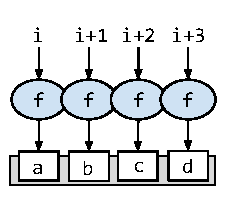
\includegraphics[width=3.0cm]{figs/Map.pdf}  }&
% \belowbaseline[-20pt]{ 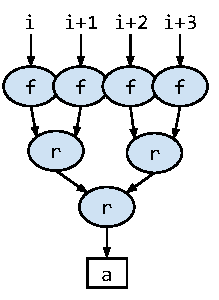
\includegraphics[width=3.0cm]{figs/Reduce.pdf}  }&
% \belowbaseline[-20pt]{ 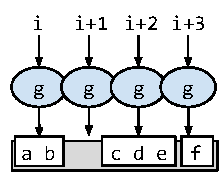
\includegraphics[width=3.0cm]{figs/FlatMap.pdf} }&
% \belowbaseline[-20pt]{ 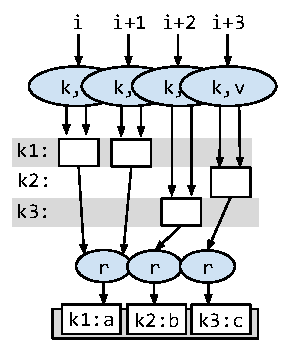
\includegraphics[width=3.9cm]{figs/HashReduce.pdf} }\\
% \midrule

% Compute &
% \multicolumn{4}{c}{\begin{tabular}[c]{@{}c@{}}Pipelined, programmable compute\\ SIMD lanes\end{tabular}} \\
% \midrule

% % On-chip Memory
% \multirow{2}{*}{\begin{tabular}[c]{@{}l@{}}On-Chip\\ Memory\end{tabular}} &
%   \multicolumn{4}{c}{\begin{tabular}[c]{@{}c@{}}Distributed register files (intermediate scalars)\end{tabular}} \\
% & \multicolumn{4}{c}{\begin{tabular}[c]{@{}c@{}}Double buffering support\end{tabular}} \\
% \cline{2-5}

% & \multicolumn{1}{c|}{\begin{tabular}[c]{@{}c@{}}Banked scratchpads\end{tabular}} &
%   \multicolumn{1}{c|}{} &
%   \multicolumn{1}{c|}{\begin{tabular}[c]{@{}c@{}}Banked FIFO\\memories \end{tabular}} &
%   \multicolumn{1}{c}{\begin{tabular}[c]{@{}c@{}}CAM (sparse)\\Banked\\scratchpads (dense)\end{tabular}} \\
% \midrule

% % Off-chip memory
% \multirow{3}{*}{\begin{tabular}[c]{@{}l@{}}Off-Chip\\ Memory\end{tabular}} &
%   \multicolumn{4}{c}{\begin{tabular}[c]{@{}c@{}}Burst commands (linear reads and writes)\end{tabular}} \\ %\cline{2-5}
% & \multicolumn{4}{c}{\begin{tabular}[c]{@{}c@{}}Gather support (random reads)\end{tabular}} \\ %\cline{2-5}
% & \multicolumn{4}{c}{\begin{tabular}[c]{@{}c@{}}Scatter support (random writes)\end{tabular}} \\ %\cline{2-5}
% %& \multicolumn{4}{c}{\begin{tabular}[c]{@{}c@{}}Address coalescing to minimize DRAM requests\end{tabular}} \\ %\cline{2-5}
% %& \multicolumn{4}{c}{\begin{tabular}[c]{@{}c@{}}Multiple outstanding memory requests to utilize memory bandwidth\end{tabular}} \\
% \midrule

% %Interconnect
% \multirow{1}{*}{\begin{tabular}[c]{@{}l@{}}Interconnect\end{tabular}} &
% \multicolumn{1}{c|}{} &
% \multicolumn{1}{c|}{Cross-lane reduction tree}&
% \multicolumn{1}{c|}{Cross-lane coalescing} &
% \multicolumn{1}{c}{} \\
% \midrule

% %Control
% \multirow{2}{*}{\begin{tabular}[c]{@{}l@{}}Control\end{tabular}} &
%   \multicolumn{4}{c}{\begin{tabular}[c]{@{}c@{}}Parallelizable counter chains for generating indices\end{tabular}} \\ %\cline{2-5}
% & \multicolumn{4}{c}{\begin{tabular}[c]{@{}c@{}}Reconfigurable control for hierarchical pipelining\end{tabular}} \\

% \bottomrule
% \end{tabular}

% \caption{The parallel patterns and their corresponding hardware implementation requirements}
% \label{t:patterns}
% \end{table*}


Parallel patterns are an extension to traditional functional programming which capture parallelizable computation on both dense and sparse data collections along with corresponding memory access patterns.
Parallel patterns enable simple, automatic program parallelization rules for common computation tasks
while also improving programmer productivity through higher level abstractions.
The performance benefit from parallelization, coupled with improved programmer productivity, has caused parallel patterns to become increasingly popular in a variety of domains,
including machine learning, graph processing, and database analytics~\cite{ecoop13sujeeth,pldi13halide}.
Previous work has shown how parallel patterns can be used in functional programming models to generate multi-threaded
C++ for CPUs comparable to hand optimized code~\cite{delite-tecs14} and efficient accelerator designs for FPGAs~\cite{auerbach10lime,george14fpl,delite2maxj}.
As with FPGAs and multi-core CPUs, knowledge of data parallelism is vital to achieve good performance when targeting CGRAs.
This implicit knowledge makes parallel patterns a natural programming model to drive CGRA design.

Like previous work on hardware generation from parallel patterns~\cite{george14fpl,delite2maxj}, our programming model is based on 
the parallel patterns \emph{Map}, \emph{FlatMap}, \emph{Fold}, and \emph{HashReduce}. These patterns are selected because they are most amenable to hardware acceleration.
Table~\ref{t:patterns} depicts conceptual examples of each pattern, where computation is shown operating on four indices simultaneously.
Every pattern takes as input one or more functions and an \emph{index domain} describing the range of values that the pattern operates over.
Each of these patterns builds an output and reads from an arbitrary number of input collections.


\emph{Map} creates a single output element per index using the function \emph{f}, where each execution of \emph{f} is guaranteed to be independent.
The number of output elements from Map is the same as the size of the input iteration domain.
Based on the number of collections read in \emph{f} and the access patterns of each read, Map can capture the behavior of a gather, a standard element-wise map, a zip, a windowed filter, or any combination thereof.

\emph{FlatMap} produces an arbitrary number of elements per index using function \emph{g}, where again function execution is independent. The produced elements are concatenated into a flat output. Conditional data selection (e.g. \emph{WHERE} in SQL, \emph{filter} in Haskell or Scala) is a special case of FlatMap where \emph{g} produces zero or one elements.

\emph{Fold} first acts as a Map, producing a single element per index using the function \emph{f}, then reduces these elements using an associative combine function \emph{r}.

\emph{HashReduce} generates a hash key and a value for every index using functions \emph{k} and \emph{v}, respectively. Values with the same corresponding key are reduced on the fly into a single accumulator using an associative combine function \emph{r}. HashReduce may either be dense, where the space of keys is known ahead of time and all accumulators can be statically allocated, or sparse, where the pattern may generate an arbitrary number of keys at runtime. Histogram creation is a common, simple example of HashReduce where the \emph{key} function gives the histogram bin, the \emph{value} function is defined to always be "1", and the \emph{combine} function is integer addition.

    %// (*@\emph{\textbf{Outer Map function (f1)}} @*) 
      %// (*@\emph{\textbf{Inner map function (f2)}} @*) 
      %// (*@\emph{\textbf{Combine function (r)}} @*)
\begin{figure}\centering
\begin{lstlisting}[language=Scala]
val a: Matrix[Float]  // M x N
val b: Matrix[Float]  // N x P
val c = Map(M, P){(i,j) =>
  // Outer Map function (f1)
  Fold(N)(0.0f){k =>
    // Inner map function (f2)
    a(i,k) * b(k,j)
  }{(x,y) =>
    // Combine function (r)
    x + y
  }
}
\end{lstlisting}
\vspace{-10pt}
\caption{Example of using Map and Fold in a Scala-based language for computing an untiled matrix multiplication using inner products. }
\label{fig:matmult}
%\vspace{-10pt}
\end{figure}

  %// (*@\emph{\textbf{Key function (k)}} @*)
  %// (*@\emph{\textbf{Value function (v)}} @*)
  %// (*@\emph{\textbf{Combine function (r) - combine using summation}} @*)
\begin{figure}\centering
\begin{lstlisting}[language=Scala]
val CUTOFF: Int = Date("1998-12-01")
val lineItems: Array[LineItem] = ...
val before = lineItems.filter{ item => item.date < CUTOFF }

val query = before.hashReduce{ item =>
  // Key function (k)
  (item.returnFlag, item.lineStatus)
}{ item =>
  // Value function (v)
  val quantity = item.quantity
  val price = item.extendedPrice
  val discount = item.discount
  val discountPrice = price * (1.0 - discount)
  val charge = price * (1.0 - discount) * (1.0 + item.tax)
  val count = 1
  (quantity, price, discount, discountedPrice, count)
}{ (a,b) =>
  // Combine function (r) - combine using summation
  val quantity = a.quantity + b.quantity
  val price = a.price + b.price
  val discount = a.discount + b.discount
  val discountPrice = a.discountPrice + b.discountPrice
  val count = a.count + b.count
  (quantity, price, discount, discountPrice, count)
}
\end{lstlisting}
\vspace{-10pt}
\caption{Example of using filter (FlatMap) and HashReduce in a Scala-based language, inspired by TPC-H query 1. }
\label{fig:tpchq1}
\vspace{-5pt}
\end{figure}

%%% Code example explanation
Figure~\ref{fig:matmult} shows an example of writing an untiled matrix
multiplication with an explicit parallel pattern creation syntax. In
this case, the Map creates an output matrix of size \texttt{M}~$\times$~\texttt{P}. 
The Fold produces each element of this matrix using a dot product over \texttt{N} elements.
Fold's map function (\texttt{f2}) accesses an element of matrix \texttt{a} and matrix \texttt{b} and multiplies them.
Fold's combine function (\texttt{r}) defines how to combine arbitrary elements produced by \texttt{f2}, in this case using summation.


Figure~\ref{fig:tpchq1} gives an example of using parallel patterns in a Scala-based language, where infix operators have been
defined on collections which correspond to instantiations of parallel patterns. Note that in this example, the \texttt{filter} on line 3 creates
a FlatMap with an index domain equal to the size of the \texttt{lineItems} collection. The \texttt{hashReduce} on line 5 creates a HashReduce with an index domain with the size of the \texttt{before} collection.



%\christos{For the memory patterns, I'd say
%  bank scratchpad (X) where X is the access pattern (FIFO, etc). The
%  off-chip memory entry is confusing as it does not say which pattern
%  uses which feature}\christos{You can trim 2.1 if needed}


\subsection{Hardware Implementation Requirements}
Parallel patterns provide a concise set of parallel abstractions that can succinctly express a wide variety of 
machine learning and data analytic algorithms \cite{ecoop13sujeeth, pldi13halide, catanzaro11copperhead, delite2maxj}.
By creating an architecture with specialized support for these patterns, we can execute these algorithms efficiently.
This parallel pattern architecture requires several key hardware features, described below and summarized in Table~\ref{t:requirements}.

%We would like our reconfigurable hardware accelerator to be able to take advantage of the high level programming and compiler information granted by parallel patterns.
%To most efficiently support these patterns, the hardware should have a variety of architectural features, summarized in Table~\ref{t:patterns}.

\begin{table}[]
\centering
\resizebox{0.95\columnwidth}{!}{%
\begin{tabular}{rcc}
\toprule
{} & \small{\textbf{Programming Model}} & \small{\textbf{Hardware}} \\
\midrule

\footnotesize

\multirow{2}{*}{\begin{tabular}[c]{@{}l@{}}\small{\textbf{Compute}}\end{tabular}} &
\multirow{2}{*}{\begin{tabular}[c]{@{}c@{}}\small{Parallel patterns}\end{tabular}} &
\small{Pipelined compute} \\
& &{\begin{tabular}[c]{@{}c@{}}\small{SIMD lanes}\end{tabular}} \\
\midrule

\multirow{5}{*}{\begin{tabular}[c]{@{}l@{}}\small{\textbf{On-Chip}}\\ \small{\textbf{Memory}}\end{tabular}} &
     \small{Intermediate scalars} & \small{Distributed pipeline registers} \\
{} & \small{Tiled, linear accesses} & \small{Banked scratchpads} \\
{} & \small{Random reads} & \small{Duplicated scratchpads} \\
{} & \small{Streaming, linear accesses} & \small{Banked FIFOs} \\
{} & \small{Nested patterns} & \small{Double buffering support} \\
\midrule

\multirow{2}{*}{\begin{tabular}[c]{@{}l@{}}\small{\textbf{Off-Chip}}\\\small{\textbf{Memory}}\end{tabular}} &
  \small{Linear accesses} & \small{Burst commands} \\
{} & \small{Random reads/writes}  & \small{Gather/scatter support} \\
%{} & \small{Random writes} & \small{Scatter support} \\
\midrule

\multirow{2}{*}{\begin{tabular}[c]{@{}l@{}}\small{\textbf{Interconnect}}\end{tabular}} &
     \small{Fold}    & \small{Cross-lane reduction trees} \\
{} & \small{FlatMap} & \small{Cross-lane coalescing} \\
\midrule

\multirow{2}{*}{\begin{tabular}[c]{@{}l@{}}\small{\textbf{Control}}\end{tabular}} &
     \small{Pattern indices} & \small{Parallelizable counter chains} \\
{} & \small{Nested patterns} & \small{Programmable control} \\
\bottomrule
\end{tabular}
}

\caption{Programming model components and their corresponding hardware implementation requirements.}
\label{t:requirements}
\vspace{-20pt}
\end{table}

First, all four patterns express data-parallel computation where operations on each index are entirely independent.
An architecture with pipelined compute organized into SIMD lanes exploits this data parallelism to achieve a multi-element per cycle throughput.
Additionally, apart from the lack of loop-carried dependencies, we see that functions \emph{f}, \emph{g}, \emph{k}, and \emph{v} in Table~\ref{t:patterns} are otherwise unrestricted.
This means that the architecture's pipelined compute must be programmable in order to implement these functions.

Next, in order to make use of the high throughput available with pipelined SIMD lanes, the architecture must be able to deliver high on-chip memory bandwidth.
In our programming model, intermediate values used within a function are typically scalars with statically known bit widths.
These scalar values can be stored in small, distributed pipeline registers.

Collections are used to communicate data between parallel patterns.
Architectural support for these collections depends on their associated memory access patterns, determined by analyzing the function used to compute the memory's address.
For simplicity, we categorize access patterns as either statically predictable \emph{linear} functions of the pattern indices or unpredictable, \emph{random} accesses.
Additionally, we label accesses as either \emph{streaming}, where no data reuse occurs across a statically determinable number of function executions, or \emph{tiled}, where reuse may occur.
We use domain knowledge and compiler heuristics to determine if a random access may exhibit reuse.
Previous work has shown how to tile parallel patterns to introduce statically sized windows of reuse into the application and potentially increase data locality \cite{delite2maxj}.

%Tiling computation with parallel patterns has previously been shown to improve the number of accesses
%Previous work has also shown how to tile parallel patterns to break up computation into fixed size units and increase the number of accesses with reuse.\cite{delite2maxj}.

Collections with tiled accesses can be stored in local scratchpads.
To drive SIMD computation, these scratchpads should support multiple parallel address streams when possible.
In the case of linear accesses, address streams can be created by banking.
Parallel random reads can be supported by local memory duplication, while random write commands must be sequentialized and coalesced.

Although streaming accesses inevitably require going to main memory, the cost of main memory reads and writes can be minimized by coalescing memory commands and prefetching
data with linear accesses. Local FIFOs in the architecture provide backing storage for both of these optimizations.

%However, local memories can help to store intermediate values to reduce the total number of expensive off-chip accesses.

%Note that for hardware, the distinction of statically known number of executions is important, as this directly corresponds to the size





%%Previous work has shown how to tile parallel patterns to potentially improve locality .
%Collections with streaming accesses can be implemented in the architecture as FIFOs.




%In many algorithms, the patterns can also be tiled

%If the address range is known to be small, memories with linear and random accesses can be implemented as scratchpads.
%A dense HashReduce, for example, exhibits random writes to its output collection, but often within a small, statically known address size.
%Additionally, computation can often be reorganized to work
%Otherwise, caches or content-addressable memories (CAMs) are necessary to store local copies of data.

These local memories allow us to exploit locality
in the application in order to minimize the number of costly loads or
stores to main memory \cite{dark}. Reconfigurable banking support within these
local memories increases the bandwidth available from these on-chip
memories, thus allowing better utilization of the compute. Double
buffering, generalized as \emph{N}-buffering, support in scratchpads
enables coarse-grain pipelined execution of imperfectly nested
patterns.

%In all four parallel patterns, if the output collection is dense, writing to the output collection has a ``sequential'' access pattern.
%Writing to sparse outputs is equivalent to a scatter.

The architecture also requires efficient memory controllers to populate local memories and commit calculated results.
As with on-chip memories, the memory controller should be specialized to different access patterns.
Linear accesses correspond to DRAM burst commands, while random reads and writes in parallel patterns correspond to gathers and scatters, respectively.



%For data structures, the architecture required to achieve high bandwidth depends on the data's memory access patterns.
%Predictable, linear access patterns are common in applications working with dense data structures, while random, data dependent accesses are common for sparse data.
%Dense Map and FlatMap, for example, always have linear writes to their output collections, while sparse Map and HashReduce always write randomly.
%\todo{Linear accesses -> burst access support to main memory} Gather and scatter are also common, especially for sparse data structures, and can be supported in the architecture through dedicated scatter/gather memory control support, command coalescing of random accesses, and support for a large number of outstanding memory requests.

Fold and FlatMap also suggest fine-grained communication across SIMD lanes. Fold requires reduction trees across lanes, while the concatenation in FlatMap is best supported by valid word coalescing hardware across lanes.

Finally, all parallel patterns have one or more associated loop indices. These indices can be implemented in hardware as parallelizable, programmable counter chains.
Since parallel patterns can be arbitrarily nested, the architecture must also have programmable control logic to determine when each pattern is allowed to execute.

While many coarse-grained hardware accelerators have been proposed, no single accelerator described by previous work has all of these hardware features.
This means that, while some of these accelerators can be targeted by parallel patterns, none of them can fully exploit the properties of these patterns to achieve maximum performance.
Traditional FPGAs can also be configured to implement these patterns, but with much poorer energy efficiency, as we show in Section~\ref{evaluation}.
We discuss related work further in Section~\ref{relatedWork}.
%% Finally, have a sentence that it can
  %all be done with a fine-grain FPGA but the overheads are huge as all
%coarse-grain array work has shown.}

\section{The Plasticine Architecture}
\label{plasticine}
Plasticine is a tiled architecture consisting of reconfigurable \emph{Pattern
Compute Units} (PCUs) and \emph{Pattern Memory Units} (PMUs), which we refer to collectively simply as ``units''. Units communicate with three kinds of static
interconnect: word-level scalar, multiple-word-level vector, and bit-level control interconnects.
Plasticine's array of units interfaces with DRAM through multiple DDR channels. Each channel has an associated
address management unit that arbitrates between multiple address streams, and consists of buffers
to support multiple outstanding memory requests and address coalescing to minimize DRAM accesses.
Each Plasticine component is used to map specific parts of applications: local address calculation is done in PMUs, DRAM address computation happens in the DRAM address management units, and the remaining data computation happens in PCUs.
Note that the Plasticine architecture is parameterized; we discuss the sizing of these parameters in Section~\ref{sizing_section}

% The following sections describe the
% datapath, control, interconnect, and the execution model in greater
% detail.
\begin{figure*}[ht]
  \centering
  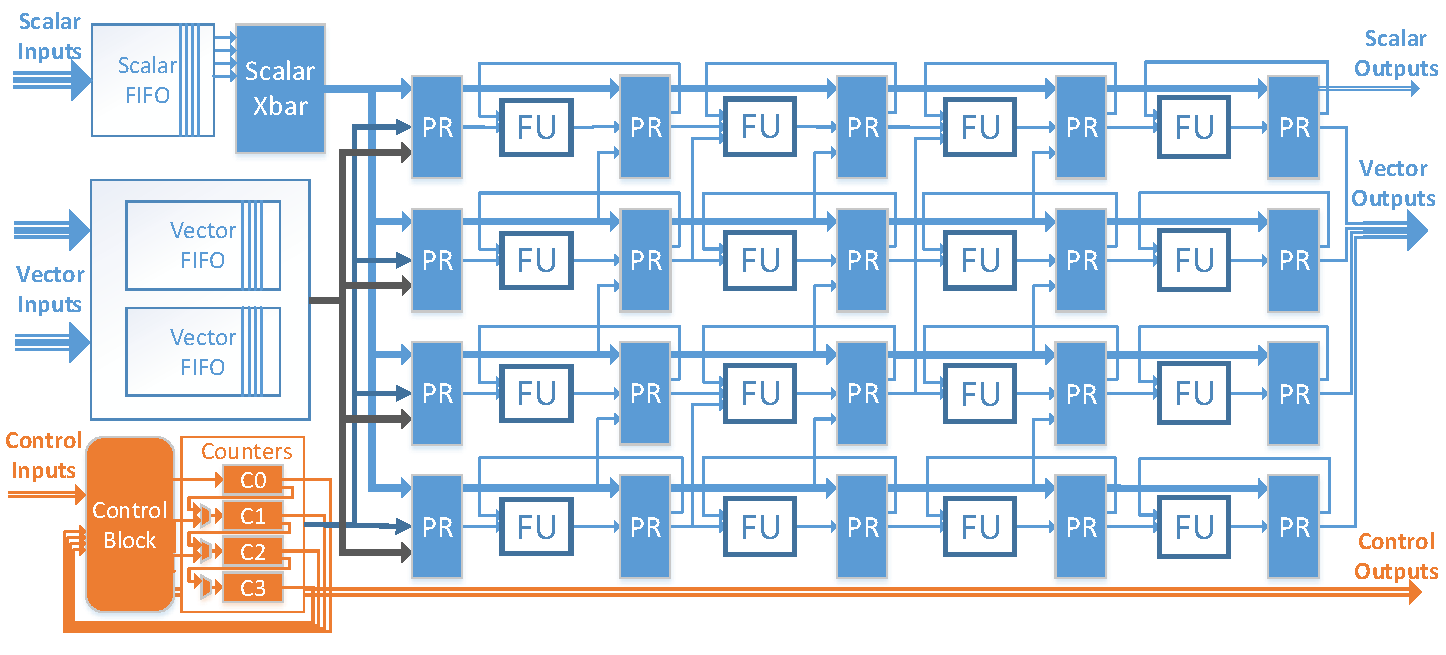
\includegraphics[width=0.82\textwidth]{figs/plasticineV2_simple.pdf}
  \vspace{-10pt}
  \caption{Pattern Compute Unit (PCU) architecture. We show only 4 stages and 4 SIMD lanes, and omit some control signals.
  \vspace{3pt}
}\label{fig:pcu}
\end{figure*}

\begin{figure*}[ht]
\centering
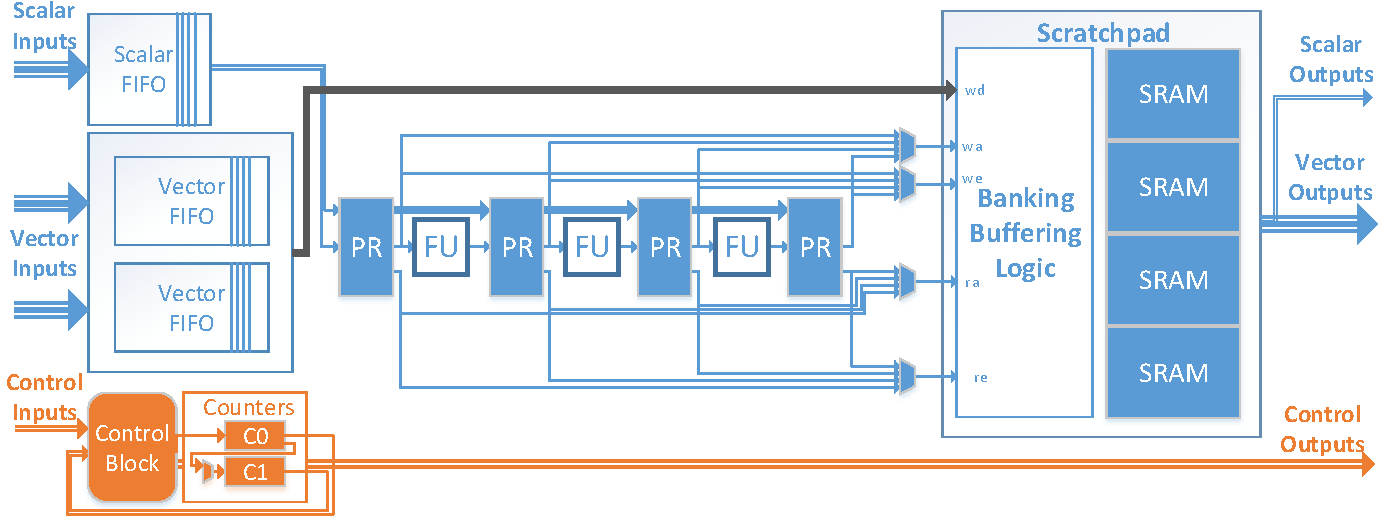
\includegraphics[width=0.82\textwidth]{figs/pmu.pdf}
  \vspace{-10pt}
  \caption{Pattern Memory Unit (PMU) architecture: configurable scratchpad, address calculation datapath, and control.}
  \label{fig:pmu}
  \vspace{3pt}
\end{figure*}

\begin{figure*}[ht]
\centering
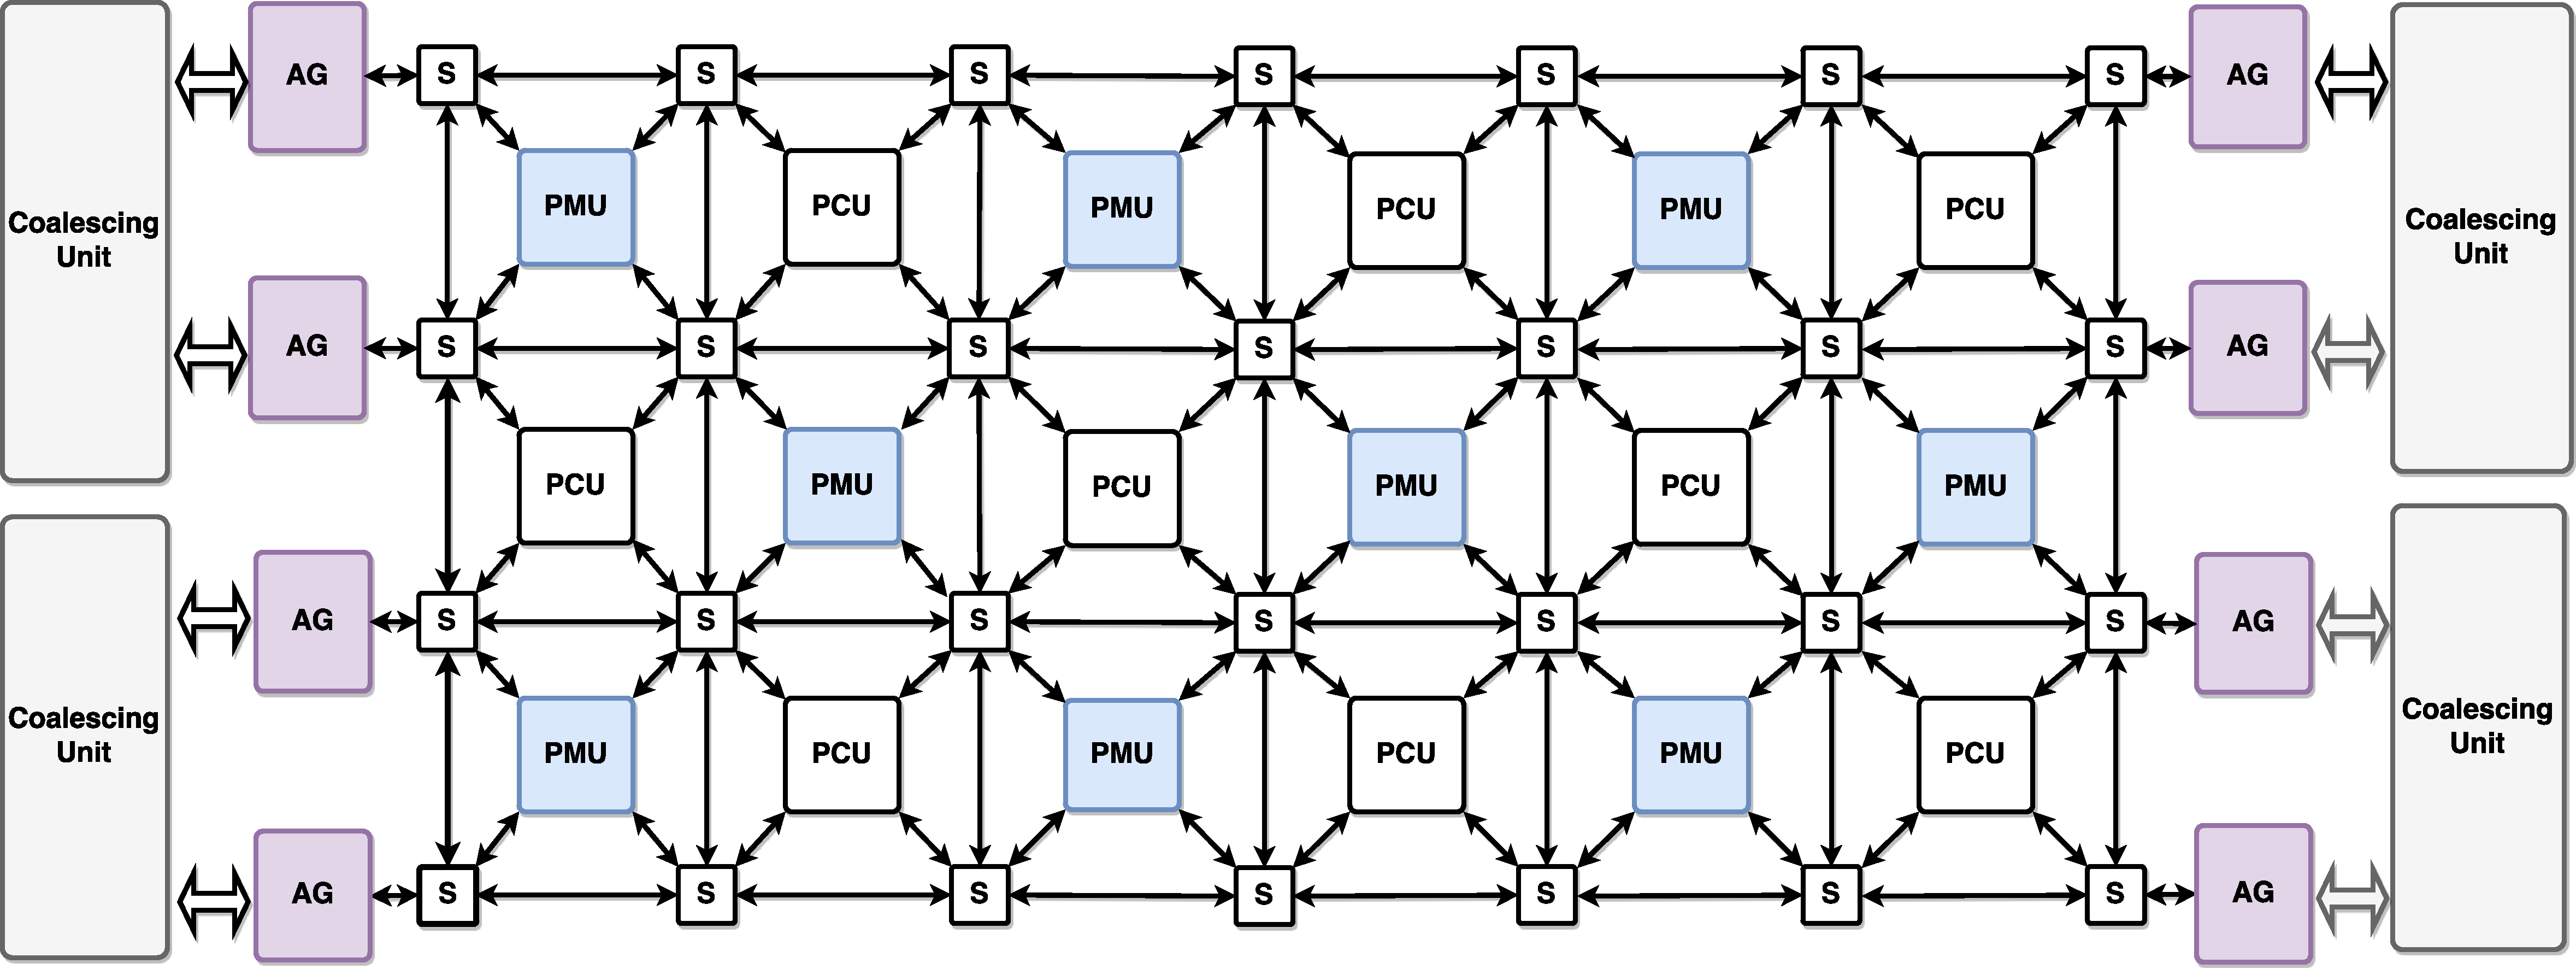
\includegraphics[width=0.9 \textwidth]{figs/network.pdf}
  \vspace{-10pt}
  \caption{Plasticine chip-level architecture (actual organization 16 x 8). All three networks have
  the same structure. \\
  PCU:Pattern Compute Unit, PMU: Pattern Memory Unit, AG: Address Generator, S: Switch Box.}
  \label{fig:interconnect}
  \vspace{0pt}
\end{figure*}
 %\vspace{-20pt}

\subsection{Pattern Compute Unit}
\label{ssec:PCU}
% \gist {Describe PCU datapath: Reconfigurable, pipelined SIMD stages, pipeline registers, counter chain.
% Describe connectivity between FUs: pipelined communication between stages, reduction tree across
% lanes, shift network between lanes. Control block consists of a few up-down counters and reconfigurable
% 'and' trees to co-ordinate with other PCUs.

% PCU and external world: PCU has 3 kinds of IO: scalar, vector, and control. Scalar and vector inputs
% are buffered using FIFOs at the input to decouple data producers and consumers.
% }

The PCU is designed to execute a single, innermost parallel pattern in
an application. As shown in Figure~\ref{fig:pcu}, the PCU datapath is organized as a multi-stage, reconfigurable SIMD pipeline.
This design enables each PCU to achieve high compute density, and exploit both loop-level
parallelism across lanes and pipeline parallelism across stages.

Each stage of each SIMD lane is composed of a \emph{functional unit} (FU) and associated pipeline registers
(PR). FUs perform
32 bit word-level arithmetic and binary operations, including support for floating point and integer operations. 
As the FUs in a single pipeline stage operate in SIMD, each stage requires only a single configuration register.
Results from each FU are written to its associated register. 
PRs in each lane are chained together across pipeline
stages to allow live values  propagate between stages within the
same lane. Cross-lane communication between FUs is captured using two types of intra-PCU networks: a reduction tree network that allows
reducing values from multiple lanes into a single scalar, and a shift network which allows using PRs as sliding windows
across stages to exploit reuse in stencil applications.
Both networks use dedicated registers within PRs to minimize hardware overhead.

PCUs interface with the global interconnect using three kinds of inputs and outputs (IO); scalar, vector, and control. Scalar IO is used to communicate
single words of data, such as the results of Folds. Each vector IO allows communicating one word per lane in the PCU, and is used in cases such as
reading and writing to scratchpads in PMUs and transmitting intermediate data across a long pipeline between multiple PCUs.
Each vector and scalar input is buffered using a small FIFO. Using input FIFOs decouples data producers and consumers, and simplifies inter-PCU control
logic by making it robust to input delay mismatches. Control IO is used to communicate control signals such as the start or end of execution of a PCU,
or to indicate backpressure.

A reconfigurable chain of counters generates pattern iteration
indices and control signals to coordinate execution. PCU execution begins when the control block enables one of the
counters. Based on the application's control and data dependencies, the control block can be configured to combine
multiple control signals from both local FIFOs and global control inputs to trigger PCU execution.
The control block is implemented using reconfigurable combinational logic and programmable up-down counters
for state machines.


\begin{figure*}[ht]
  \centering
  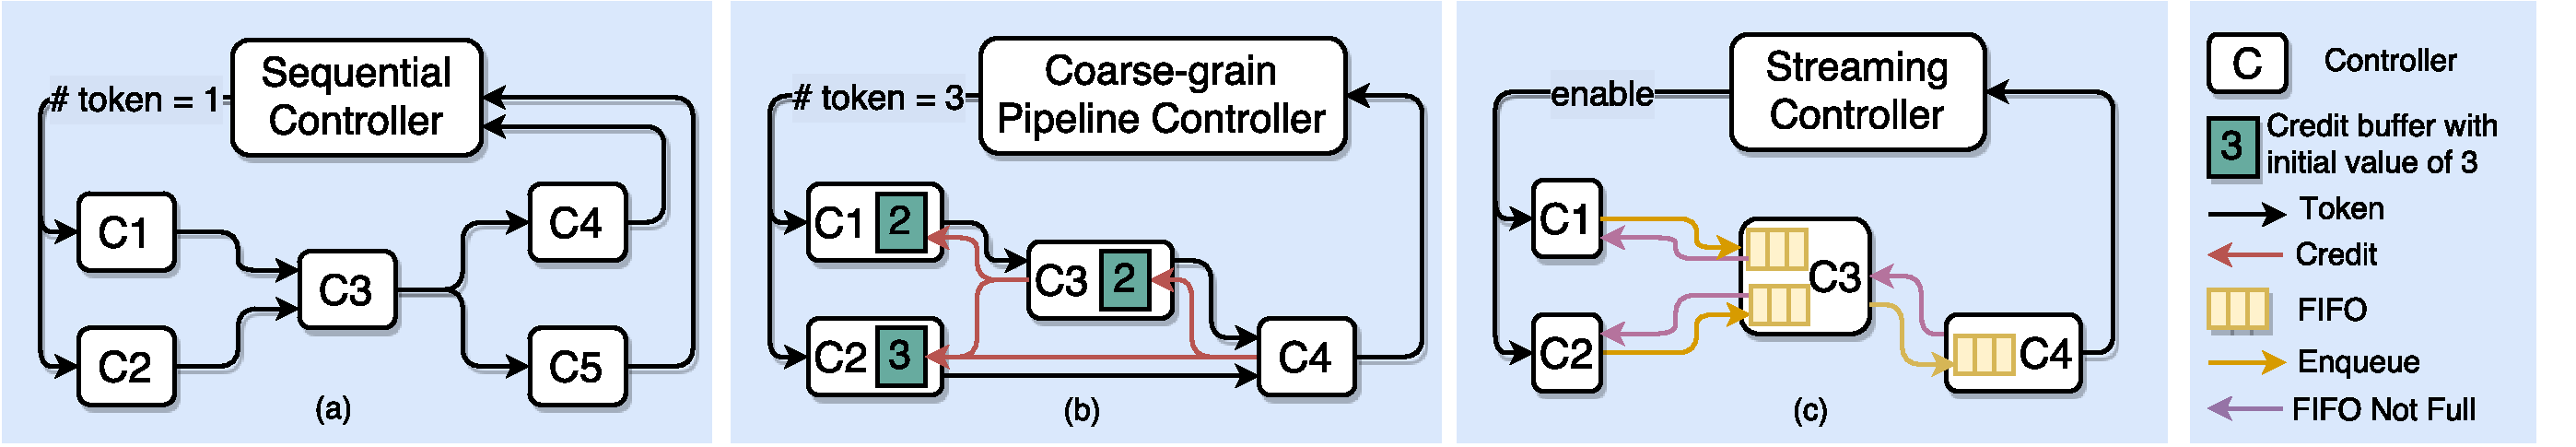
\includegraphics[width=1\textwidth]{figs/control.pdf}
  \vspace{-20pt}
  \caption{Sequential, coarse-grained pipelining, and streaming control schemes.}
  \label{fig:control}
\end{figure*}

%  Address Generators (AG) produce DRAM requests
%  into a coalescing unit, which arbitrates between AGs and coaleses requests to the same DRAM burst.
\subsection{Pattern Memory Unit}
\label{ssec:PMU}
% \gist{On-chip scratchpad with a reconfigurable integer pipeline.
%  FIFOs at inputs of PCUs and PMUs
% decouple PMU memory access from PCU execution. Scratchpad is banked with 16 banks,
% and can be configured in multiple modes to support various access patterns.
% Strided, N-buffered, FIFO, Line Buffer, Duplication etc.
% }
%For compute intensive applications, two factors need to be considered to both increase utilization and overall system energy efficiency. First, most memory accesses should be localized on the chip to decrease expensive DRAM accesses. Second, the architecture should include a memory hierarchy to lower the energy of repetitive accesses from ALUs~\cite{dark, LAP_TC12}.
%In Plasticine, memory hierarchy is supported in the form of PMUs distributed throughout the chip.
Figure~\ref{fig:pmu} shows the architecture of a PMU.
Each PMU contains a programmer-managed scratchpad memory coupled with a reconfigurable scalar datapath intended for address calculation.
As shown in Figure~\ref{fig:interconnect}, PMUs are used to distribute on-chip memory throughout the Plasticine architecture.
Plasticine makes a distinction between the operations involved in memory addresses calculation and the core computation
underlying applications. Address calculation is performed on the PMU datapath, while the core computation is performed within the PCU.
Several observations have motivated this design choice:
(i)  Address calculation involves simple scalar math, which requires simpler ALUs than the FUs in PCUs;
(ii) Using multiple lanes for address computation is often unnecessary for most on-chip access patterns; and
(iii) Performing address calculation within the PCU requires routing the addresses from the PCU to the PMU, which occupies PCU stages
     and output links, and can lead to PCU under-utilization.



The scratchpads are built with multiple SRAM banks matching the number of PCU lanes. Address decoding logic around the scratchpad
can be configured to operate in several banking modes to support various access patterns. \emph{Strided banking} mode supports
linear access patterns often found on dense data structures. \emph{FIFO} mode supports streaming accesses. \emph{Line buffer}
mode captures access patterns resembling a sliding window. \emph{Duplication} mode, where the contents are duplicated across all
memory banks, provides multiple read address channels to support parallelized on-chip gather operations.

Just as banking is important to feed multiple SIMD units to sustain compute throughput, \emph{N-buffering}, or generalized double buffering,
is just as important to support coarse-grained pipelines. The PMU scratchpad can be configured to operate as an N-buffer with any
of the banking modes described. N-buffers are implemented by partitioning the address space in each SRAM bank into N disjoint regions.
Using write and read state information, an appropriate offset is added to each bank's local address to access the correct data.

A programmable counter chain and control block triggers PMU execution similar to the PCU. Each PMU typically contains write address
calculation logic from the producer pattern, and read address calculation logic from the consumer pattern. Based on the state of
the local FIFOs and external control inputs, the control block can be configured to trigger the write address computation, read
address computation, or both, by enabling the appropriate counters.

\subsection{Interconnect}
\label{ssec:Interconnect}
Plasticine supports communication between PMUs, PCUs, and peripheral elements using
three kinds of interconnect - scalar, vector, and control. The networks differ in the granularity of
data being transferred; scalar networks operate at word-level granularity, vector networks operate at
multiple word-level granularity, and control networks operate at bit-level granularity. The topology
of all three networks is identical, and is shown in Figure~\ref{fig:interconnect}. All networks are
statically configured. Links in network switches include registers to avoid long wire delays.

Applications commonly contain nested pipelines, where the outer pipeline levels 
only require counters and some reconfigurable control. In addition, as outer pipeline logic
typically involves some level of control signal synchronization, they are control hotspots
which require a large number of control and scalar inputs and outputs. To handle outer pipeline logic in
an efficient manner, scalar and control switches share a reconfigurable control block and counters.
Incorporating control
logic within switches reduces routing to hotspots and increases PCU utilization.




\subsection{Off-chip Memory Access}
\label{ssec:Off-chip}
Off-chip DRAM is accessed from Plasticine using 4 DDR memory channels.
Each DRAM channel is accessed using several \emph{address generators} (AG) on two sides of the chip, as shown in Figure~\ref{fig:interconnect}.
Each AG contains a reconfigurable scalar datapath to generate DRAM requests, 
similar in structure to the PMU datapath shown in Figure~\ref{fig:pmu}. In addition, each AG contains FIFOs
to buffer outgoing commands, data, and incoming responses from DRAM. Multiple AGs connect to an address coalescing unit,
which arbitrates between the AGs and processes memory requests.

AGs can generate memory commands that are either \emph{dense} or \emph{sparse}. Dense requests are used to bulk transfer
contiguous DRAM regions, and are commonly used to read or write tiles of data. Dense requests are converted
to multiple DRAM burst requests by the coalescing unit. Sparse requests enqueue a stream of addresses into the coalescing
unit. The coalescing unit uses a coalescing cache to maintain metadata on issued DRAM requests and combines sparse
addresses that belong to the same DRAM request to minimize the number of issued DRAM requests. In other words, sparse memory loads trigger
a \emph{gather} operation in the coalescing unit, and sparse memory stores trigger a \emph{scatter} operation.



\subsection{Control Flow}
\label{ssec:Control}
%Plasticine uses a distributed \emph{token} and \emph{credit} based protocol to orchestrate control flow between PCUs and PMUs. 
%Tokens refer to feed-forward control flow signals, which are used to track the amount of data a PCU or PMU currently has available to operate on. Credits are signals which indicate back-pressure. They tell the PCU how many elements it can produce before its consumers will no longer be able to buffer its outputs. A unit can therefore execute when it has at least one token from all of its inputs, and one credit from all consumer units that it is writing to. 

%The architecture of the control block in each unit is shown in Figure~\ref{fig:controlBlock}.
%Both tokens and credits are implemented as 1-bit, single-cycle pulse control signals. 
%Each unit contains a set of configurable token buffers to track
%remaining tokens from each of its inputs.

%Figure~\ref{fig:ctrl} depicts the control logic configuration for three common outer loop control schemes: (a) \emph{sequential} execution, (b) \emph{coarse-grain pipelining}, and (c) \emph{streaming}. These control schemes correspond to outer loops in the input program, and determine how the execution of individual units are scheduled relative to other units. 
%In a sequential control flow, only one unit is active at any time.
%Therefore, when a parent controller receives a token, it will send
%a signal to initialize the first stage. 
%In coarse-grain pipelining, execution of stages is overlapped, the
%token buffer in each unit is initialized to the number of dependent pipeline stages. 
%Additionally, a credit buffer
%is allocated for any output the unit writes with an initialization of 2 to indicate double buffering at
%the consumer side. 
%Finally, in streaming, data
%dependencies between units are only enforced by states of FIFOs. In this scheme, a given unit is enabled to execute only if
%all of its input FIFOs are not empty, and all FIFOs it writes to are not full.

Plasticine uses a distributed and hierarchical control scheme that minimizes synchronization
between units in order to adapt to limited bit-wise connectivity in the interconnect. We support 
three types of controller protocols inferred from our high-level language constructs: (a) \emph{sequential} execution,
(b) \emph{coarse-grained pipelining}, and (c) \emph{streaming} (Figure~\ref{fig:control}).
These control schemes correspond to outer
loops in the input program, and determine how the execution of individual units are scheduled
relative to other units. Units are grouped into hierarchical sets of controllers. The control
scheme of sibling controllers is based on the scheme of their immediate parent controller.

In a sequential parent controller, only one data dependent child is active at any time.
This is commonly used when a program has loop-carried dependencies. To enforce data dependencies, we use
\emph{tokens}, which are feed-forward pulse signals routed through the control network. When the parent
controller is enabled, a single token is sent to all \emph{head} children with no data dependencies on their siblings. Upon
completing execution, each child then passes its token to consumers of its output data. Each
controller is enabled only when tokens from all dependent data sources are collected. 
Tokens from the last
set of controllers, whose data are not consumed by any sibling controller in the same level of hierarchy, are
sent back to the parent. The parent combines the tokens and either sends tokens back
to the heads for the next iteration, or passes the token along at its own hierarchy level when all
of its iterations have finished. 

In coarse-grained pipelines, child controllers 
are executed in a pipelined fashion. To allow concurrent execution, the parent controller sends \emph{N} \emph{tokens}
to the \emph{heads}, where \emph{N} is the number of data dependent children in the critical path. This
allows all children to be active in the steady state. To allow producers and consumers to work on
the same data across different iterations, each intermediate memory is \emph{M}-buffered, where \emph{M} is the
distance between the corresponding producer and consumer on their data dependency path. To prevent producers from
overflowing the down-stream buffer, each child controller handles backpressure by keeping
track of available down-stream buffer sizes using \emph{credits}.
The number of credits is statically initialized to M. Each producer decrements its credit count after producing
all the data for the ``current" iteration of the parent. Similarly, the consumer sends a credit back through the
network after consuming all the data for the ``current" iteration of the parent. 
In the coarse-grained pipelining scheme, each child is enabled when it has at least one token and one credit
available. 

Finally, child controllers with a \emph{streaming} parent controller
execute in a fine-grain pipelining fashion. This allows the compiler to fit a large inner pattern body by
concatenating multiple units to form a large pipeline. In streaming mode, children communicate
through FIFOs. A controller is enabled when all FIFOs it reads from are \emph{not
empty} and
all FIFOs it writes to are \emph{not full}. FIFOs are local to the consumer controller, so 
\emph{enqueue} and \emph{not empty} signals are routed from consumer to producer through the control network. 

To enforce these control protocols, we implement specialized reconfigurable control blocks using statically programmable counters,
state machines and combinational lookup tables. Each PCU, PMU, switch, and memory controller in the architecture has a control block. 
In general, controllers without any children are mapped to PCUs, while outer controllers are mapped to control logic in switches.
This mapping gives outer controllers, which often have many children to synchronize with, a higher radix for
communication. The hierarchy and distributed communication in Plasticine's control scheme allows the
compiler to leverage the multiple levels of parallelism available in nested parallel patterns with only minimum overhead from bit-level 
reconfigurability. 

%\emph{Up-down} counters in the control block track the number of tokens and credits from other units. 
%Each up-down counter provides 1-bit \emph{valid} and \emph{done} outputs, which signal when the counter is running and saturated, respectively. Look-up tables are used to combine valid signals and generate
%counter enable signals. 
%Done signals are similarly combined using look-up tables
%to generate one or more output tokens and/or credits. These control signals are sent out to other units using the control interconnect.

%Each PCU has an input control bus with several bits to carry input
%\emph{tokens}/\emph{credits}, and an output bus to carry several output
%\emph{tokens}/\emph{credits}. A main control block provides memory-mapped command
%and status registers to the host processor that manages execution of the entire Plasticine
%array. The main control block begins execution by generating a single
%token. Execution is completed when the token is returned to the main
%control block.

%\begin{figure}[ht]
%\centering
%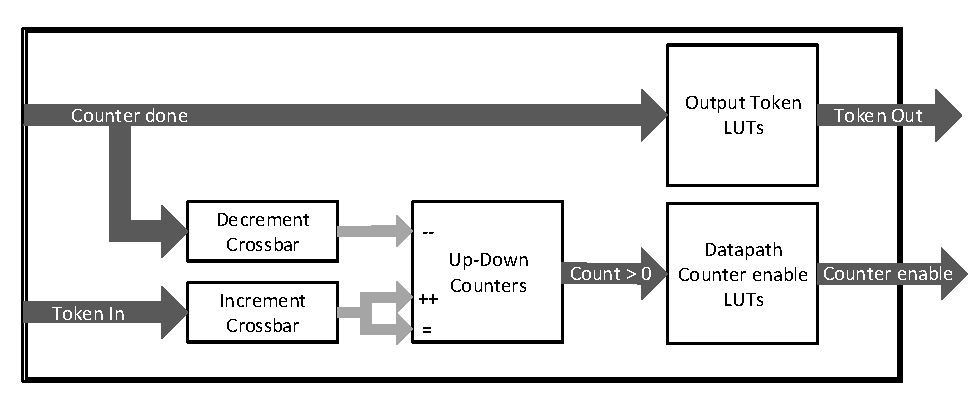
\includegraphics[width=0.45\textwidth]{figs/controlBlock.pdf}
%\caption{Control Block in a PCU.}
%\label{fig:controlBlock}
%\end{figure}

%\subsection{Memory Interfaces}
%\label{ssec:MemoryInterface}
%Several memory interfaces share a single physical DRAM channel. To optimize for
%the common case of off-chip address calculation, Plasticine has dedicated scalar
%compute units close to the memory interface.
%The PCU is designed to execute a single, potentially nested, loop of
%operations in an application. As shown in Figure~\ref{fig:cu}, the PCU
%is a multi-stage reconfigurable pipeline. Each pipeline stage includes
%a multi-lane functional unit and register set. This enables each PCU
%to achieve high compute density and exploit both loop-level
%parallelism across lanes and pipeline parallelism.  In
%Section~\ref{evaluation}, we evaluate PCUs with up to 32 stages and 4 to 32
%lanes.  Data locality is captured in each PCU using multiple
%scratchpad banks that can be statically configured to support various
%access patterns. A reconfigurable chain of counters generates of loop
%indices and control signals to coordinate execution. The counters are
%controlled by a control block, which implements the distributed
%control flow scheme for coarse-grained, task or pipeline parallel
%execution across multiple PCUs (see Section~\ref{ssec:controlflow}).
%
%
%{\bf Datapath:} The \emph{functional units} (FUs) can perform
%word-level (32b) arithmetic and logic operations. The FUs in a single
%pipeline stage operate in a SIMD, multi-lane fashion, hence requiring
%just one configuration register per stage. Each FU is associated with
%a set of pipeline registers -- denoted by the \emph{Regs} box in
%Figure~\ref{fig:cu} -- into which results from the FU are
%written. Registers in each lane are chained together across pipeline
%stages to allow live values to be propagated between stages in the
%pipeline.
%
%Table~\ref{t-cuPipeTypes} describes the different types of stages in
%each PCU. Stages are specialized in order to minimize area overheads
%without sacrificing flexibility. The first few stages in each PCU --
%like stages $0$ and $1$ in Figure~\ref{fig:cu} -- are
%\emph{read-write} stages and have maximum flexibility in choosing
%source and destination locations. \emph{Read-write} stages are
%followed by a number of \emph{regular} stages, such as Stage $2$ in
%Figure~\ref{fig:cu}, that can only consume data from previous
%stages. To support commonly occurring operations such as array
%accumulation, the last stage in each PCU is a \emph{write} stage that
%can write directly into the local scratchpads. The write address is
%obtained from a special pipeline register in the \emph{write}
%stage. \emph{Reduction} stages (Stage $3$ in Figure~\ref{fig:cu})
%implement a reduction tree across several stages to support scalar
%accumulations.
%

%
%
%\begin{table*}[]
%\centering
%\resizebox{\textwidth}{!}{%
%\begin{tabular}{@{}llll@{}}
%\bottomrule
%\textbf{Pipeline Stage Type} & \textbf{Source Locations}                                     & \textbf{Destination Locations}                          & \textbf{Inter-Lane Communication}   \\ \midrule
%Regular             & Previous Stage, Current Stage                         & Pipeline Registers                        & None                       \\ \midrule
%Read-Write          & Previous Stage, Current Stage, Scratchpads, Counters  & Pipeline Registers, Scratchpads           & None                       \\ \midrule
%Write               & Previous Stage, Current Stage                         & Pipeline Registers, Scratchpads           & None                       \\ \midrule
%Reduction           & Previous Stage, Current Stage                         & Pipeline Registers                        & Tree Network               \\ \midrule
%\end{tabular}
%}
%
%\caption{Types of PCU pipeline stages.}
%\label{t-cuPipeTypes}
%\end{table*}
%
%{\bf Scratchpad Banks:} Each local scratchpad has multiple memory
%banks to match the number of lanes in the datapath. Its capacity is in
%the few KBytes (2-32). A configurable address decoder provides a
%word-level addressing abstraction to the datapath and supports bank
%addressing schemes such as broadcast, round-robin, and strided
%modes. This allows for parallel accesses with random, sequential, and
%strided access patterns respectively. Each PCU can only read from its
%local scratchpads in the read-write pipeline stages. Scratchpads can
%be written either locally by write stages, or remotely from another
%PCU or a memory controller.
%
%{\bf Counter Chains:} Each PCU is equipped with a chain of
%reconfigurable counters to generate loop indices. Each counter can be
%configured with maximum and stride values, which can either be a
%constant or a value from one of the PCU input buses.  The counters can
%be linearly grouped into one or more chains to support
%multi-dimensional indexing found in perfectly nested loops.  For
%example, the counter chain shown in Figure~\ref{fig:cu} can be
%configured to operate as one 4-dimensional counter chain, two
%2-dimensional counter chains, or four independent counters.  Counter
%outputs are connected to the datapath as well as the scratchpad
%address ports to support linear addressing.
%
%Counters also act as the interface between data and control
%paths. Each counter can be individually managed by an `enable'
%signal. When the counter wraps around, a one-cycle `done' pulse is
%generated. The control block in each PCU generates the `enable'
%signals and uses the `done' signals to track and handle inter-PCU
%control flow.
%

%
%\subsection{Inter-PCU Interconnect}
%
%The data interconnect operates at a granularity of a vector of 16 32-bit words, or 512 bits. The control interconnect operates at a bit-level
%  granularity.
%
%Figure~\ref{fig:interconnect} shows the static interconnection topology between PCUs.
%PCUs are laid out as a two-dimensional array in a static hybrid interconnection network.
%Plasticine uses separate interconnection networks for the data path and
%control path. The data interconnect routes data at the granularity of a vector of 16
%32-bit words, or 512 bits. The control interconnect uses a bit-level interconnect to provide greater flexibility
%to route control signals between PCUs. Both interconnects have registers in the switches
%to avoid long critical paths and sustain a high clock rate.
%
%Main memory is accessed on the left and right columns of the array through reconfigurable
%memory command generators, as shown in figure~\ref{fig:interconnect}. The memory command
%generators can be configured to either operate in burst mode to optimize loading dense
%data structures, or scatter-gather mode to optimize loading sparse data structures. In
%scatter-gather mode, memory command generators support address coalescing to minimize
%off-chip DRAM access.
%
%
\subsection{Application Mapping}
\label{mapping}
We begin with an application represented as a hierarchy of parallelizable dataflow pipelines written in a parallel pattern-based language called
the Delite Hardware Definition Language (DHDL)~\cite{dhdl}.
Prior work~\cite{delite2maxj} has shown how applications expressed in the parallel patterns described in Section~\ref{patterns}
can be automatically decomposed into pipelines in DHDL.
Pipelines in DHDL are either \emph{outer controllers} which contain only other pipelines, or \emph{inner controllers} which contain no other controllers, only dataflow graphs of compute and memory operations.

To map DHDL to Plasticine, we first unroll outer pipelines using user-specified or auto-tuned parallelization factors.
The resulting unrolled representation is then used to allocate and schedule \emph{virtual} PMUs and PCUs.
These virtual units are an abstracted representation of the units in Plasticine which have an infinite number of available
inputs, outputs, registers, compute stages, and counter chains.
As outer controllers contain no computation, only control logic, they map to a virtual PCU with no compute stages, only control logic and counter chains.
The computation in inner controllers is scheduled by linearizing the data flow graph and mapping the resulting list of operations
to virtual stages and registers.
Each local memory maps to a virtual PMU. Stages used to compute read and write addresses for this memory are copied to the virtual PMUs.

We then map each virtual unit into a set of physical units by partitioning its stages.
Virtual PCUs are partitioned into multiple PCUs, while PMUs become one PMU with zero or more supporting PCUs.
While graph partitioning is NP-hard in general, each virtual unit tends to have far less than 200 compute stages with very few cyclic dependencies.
This means that a greedy algorithm with a few simple heuristics can reasonably approximate a perfect physical unit partitioning.
In our partitioning algorithm, we use a cost metric which calculates the number of physical stages, live variables per stage, and scalar and vector input/output buses required for a given partitioning.
Note that these communication and computation costs are always statically predictable because we begin with a full dataflow representation of the application.
Using our heuristics, the compiler selects a proposed partitioning
where all PCUs and PMUs are physically realizable given some chosen set of
Plasticine architecture parameters (number of PCUs, PMUs, stages, lanes, buses, etc.) and which maximize the ALU and local memory utilization.

Following partitioning, we generate the control logic corresponding to the controller hierarchy
as described in Section~\ref{ssec:Control}. We then perform hierarchical binding of virtual hardware nodes to physical hardware
resources, including datapath and control path placement and routing, register allocation of SIMD
units, including mapping stages to physical ALUs, and allocating scratchpads and control resources. The hierarchical nature of Plasticine allows us to
dramatically reduce the search space with less than 1000 nodes in each level of mapping.

Given this placement and routing information, we then generate a Plasticine configuration description, akin to an assembly language, which is
used to generate a static configuration ``bitstream'' for the architecture.
The hierarchical architecture, coupled with the coarse granularity of buses between compute units, allows our entire
compilation process to finish (or fail) in only a few minutes, as compared to the hours it can take to generate FPGA configurations.

\begin{figure*}
\centering

\begin{tabular}{p{0.01cm} p{4.6cm} p{0.01cm} p{4.6cm} p{0.01cm} p{4.6cm} p{0.9cm}}
%%% trim = right, bottom, left, top
\textbf{a.} & {\includegraphics[clip, trim=0.4cm 3.3cm 1.0cm 1.2cm, width=4.6cm]{figs/Stages.pdf}} &
\textbf{b.} & {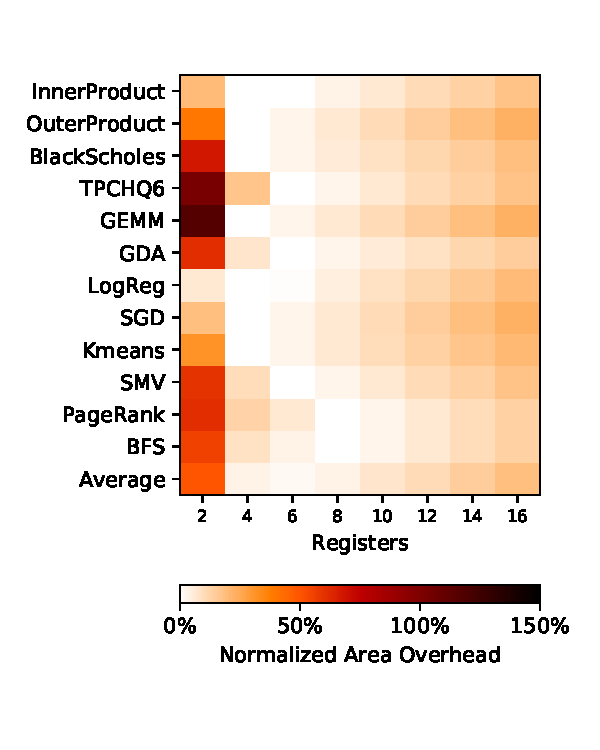
\includegraphics[clip, trim=0.4cm 3.31cm 1.0cm 1.2cm, width=4.6cm]{figs/Registers.pdf}} &
\textbf{c.} & {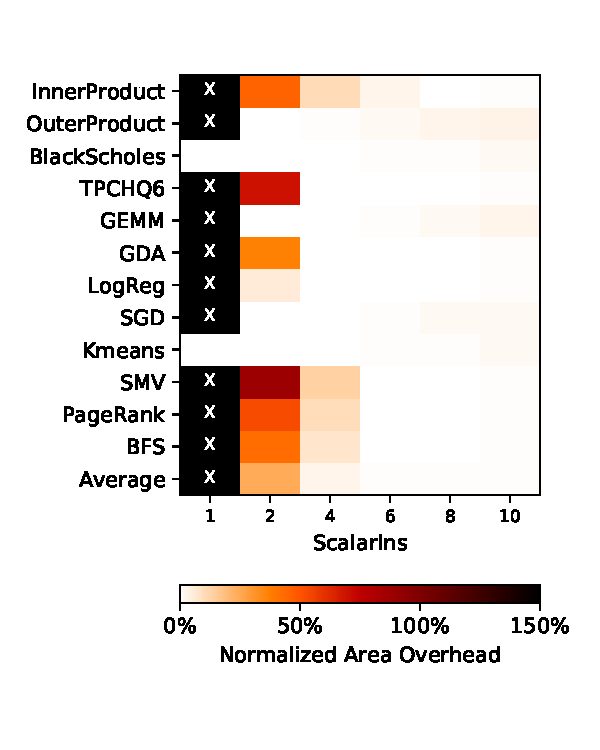
\includegraphics[clip, trim=0.4cm 3.31cm 1.0cm 1.2cm, width=4.6cm]{figs/ScalarIns.pdf}} &
{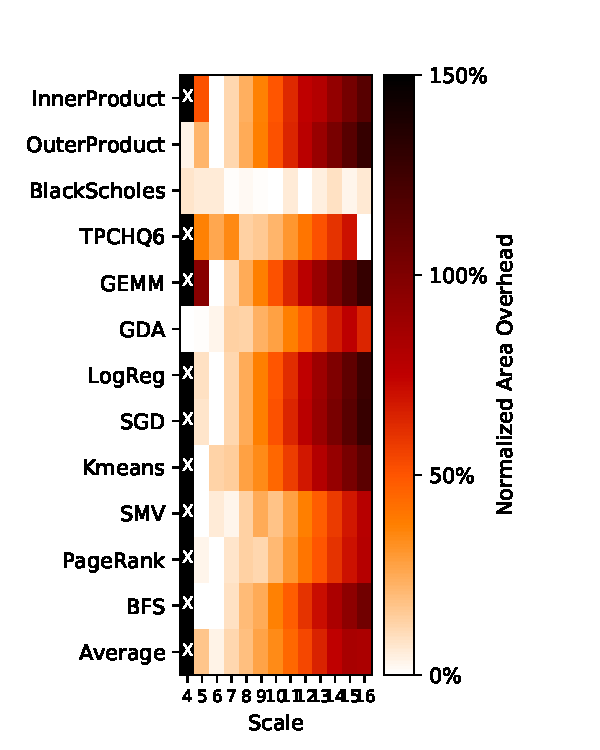
\includegraphics[clip, trim=6.4cm 0.4cm 0.4cm 0.4cm, height=4.6cm]{figs/Scale.pdf}} \\
 

\textbf{d.} & {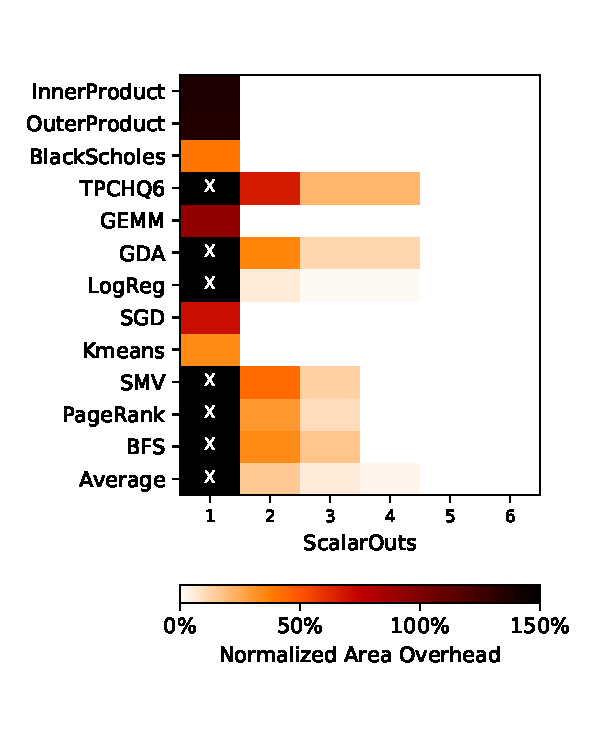
\includegraphics[clip, trim=0.4cm 3.31cm 1.0cm 1.2cm, width=4.6cm]{figs/ScalarOuts.pdf}} &
\textbf{e.} & {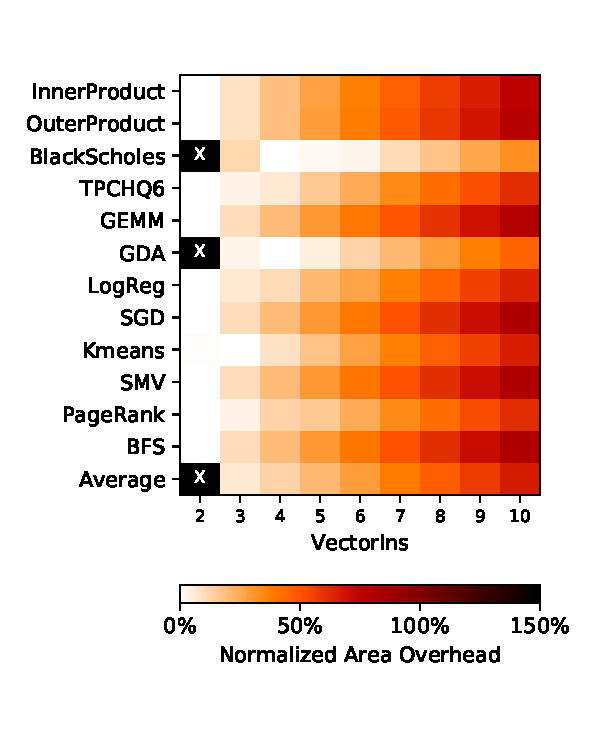
\includegraphics[clip, trim=0.4cm 3.31cm 1.0cm 1.2cm, width=4.6cm]{figs/VectorIns.pdf}} &
\textbf{f.} & {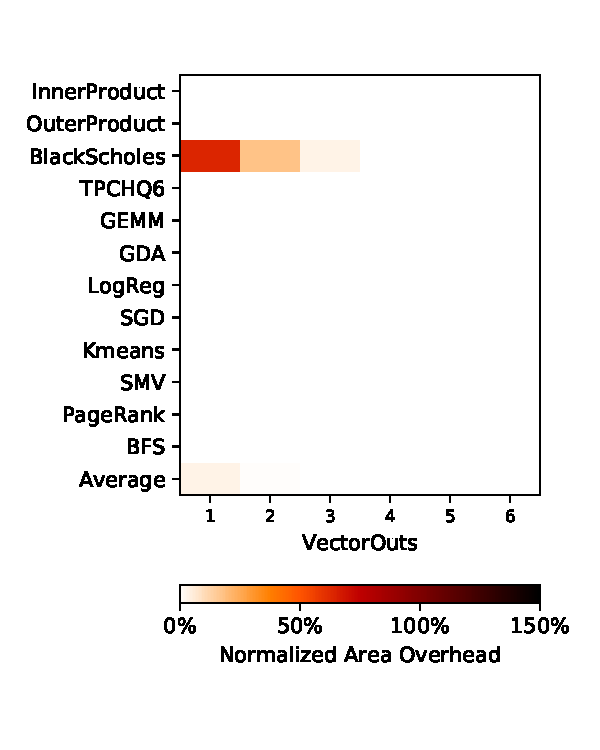
\includegraphics[clip, trim=0.4cm 3.31cm 1.0cm 1.2cm, width=4.6cm]{figs/VectorOuts.pdf}} &
{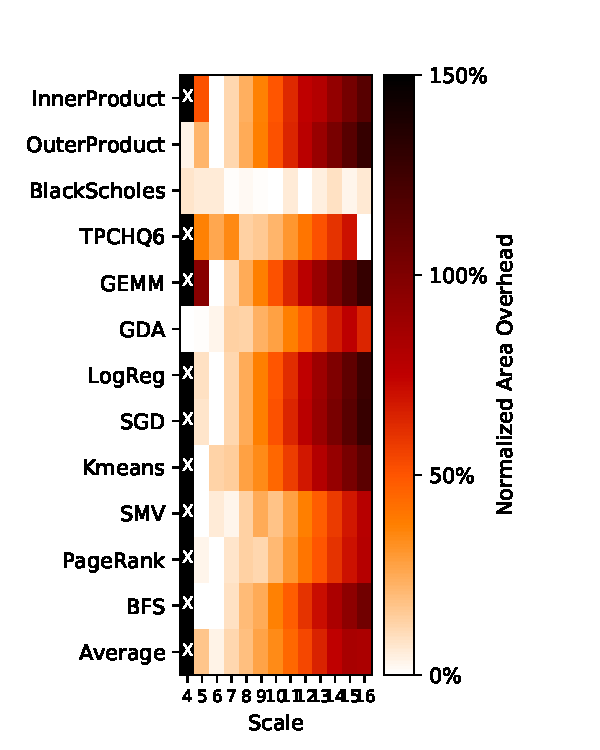
\includegraphics[clip, trim=6.4cm 0.4cm 0.4cm 0.4cm, height=4.6cm]{figs/Scale.pdf}} \\

\end{tabular}
\vspace{-10pt}
\caption{Area overhead ($Area_{PCU}/Min_{PCU} - 1$) while sweeping various Plasticine PCU parameters for a subset of our benchmarks. $Min_{PCU}$ is benchmark-specific minimum possible area. Areas marked with an $\times$ denote invalid parameters for the given application. \emph{a.}~Stages per PCU; \emph{b.}~Registers per FU with 6 stages; \emph{c.}~Scalar~inputs~per~PCU with 6 stages and 6 registers; 
\emph{d.}~Scalar~outputs~per~PCU with 6 stages, 6 registers, and 6 scalar inputs; \emph{e.}~Vector~inputs~per~PCU with 6 stages and 6 registers; and \emph{f.}~Vector~outputs~per~PCU with 6 stages, 6 registers, and 3 vector inputs. }
\label{fig:sizing}
\end{figure*}

\subsection{Architecture Sizing}
\label{sizing_section}

	%                   & \multicolumn{3}{c}{\textbf{Pattern Memory Unit}}  \\ \midrule
	%                   & \multicolumn{3}{c}{\textbf{Pattern Compute Unit}} \\ \midrule
	%                   & \multicolumn{3}{c}{\textbf{Architecture}}         \\ \midrule
\begin{table}[]
\centering
\resizebox{\columnwidth}{!}{%
\begin{tabular}{llcc}
\toprule
	                    & \textbf{Component}      & \textbf{Range}             & \textbf{Final Value} \\ \midrule
	                    & Lanes                   & 4, 8, 16, 32               & 16                   \\
	                    & Stages                  & 1 -- 16                    & 6                    \\
	\textbf{Pattern}    & Registers/Stage         & 2 -- 16                    & 6                    \\
	\textbf{Compute}    & Scalar Inputs           & 1 -- 16                    & 6                    \\
	\textbf{Unit}       & Scalar Outputs          & 1 -- 6                     & 5                    \\
	                    & Vector Inputs           & 1 -- 10                    & 3                    \\
	                    & Vector Outputs          & 1 -- 6                     & 3                    \\ \midrule
	                    & Bank Size               & 4, 8, 16, 32, 64KB         & 16KB                  \\
	                    & \emph{Scratchpad Banks} & \emph{Number of PCU Lanes} & 16                   \\
	                    & \emph{Total Scratchpad} & \emph{Bank size * banks}   & 256KB                \\
	                    & Stages                  & 1 -- 16                    & 4                    \\
	\textbf{Pattern}    & Registers/Stage         & 2 -- 16                    & 6                    \\
	\textbf{Memory}     & Scalar Inputs           & 1 -- 16                    & 4                    \\
	\textbf{Unit}       & Scalar Outputs          & 0 -- 6                     & 0                    \\
	                    & Vector Inputs           & 1 -- 10                    & 3                    \\
	                    & Vector Outputs          & 1 -- 6                     & 1                    \\ \midrule
\textbf{Architecture} & PCUs                    & ---                        & 64                   \\
	                    & PMUs                    & ---                        & 64                   \\
\bottomrule
\end{tabular}
}
\caption{Design space and final selected parameters.}
\label{t-parameters}
\vspace{-20pt}
\end{table}


%Note that in this study, we assume all PCUs and PMUs are homogeneous, i.e. we do not investagate architectures with a mix of PCU or PMU designs.
Thus far, we have described a parameterized architecture composed of, among other things, PCUs, PMUs, and interconnect.
We now describe our process for tuning the PCU and PMU parameters to create the final Plasticine architecture that we evaluate in Section~\ref{evaluation}.
Table~\ref{t-parameters} summarizes the architecture parameters under consideration, the possible values for each, and the final value we selected.
To improve the probability of application routability, we restrict PMUs and PCUs to be homogeneous across the architecture. 

In selecting design parameters, we first prune the space by analyzing the characteristics of the benchmarks listed in Table~\ref{t-apps}.
Based on models of the performance of each benchmark, we determine that the ideal inner controller parallelization factor across all benchmarks is between 8 and 32.
In Plasticine, this corresponds to Pattern Compute Units with between 8 and 32 SIMD lanes.
We select a balanced architecture with 16 lanes. Vectors of 16, 4 byte words also conveniently match our main memory's burst size of 64 bytes.
For the PMU scratchpads, we found that ideal tile sizes for our benchmarks are at most 4000 words per bank.
We therefore set the PMU to have 16 configurable, 16KB banks, for a total of 256KB~per~PMU.

We next search the remaining architectural space to select the number of stages, registers per stage, inputs, and outputs per PCU.
In our programming model, parallelizing outer controllers corresponds in hardware to duplicating inner controllers.
This means that we can assume that, to a first order, outer loop parallelization in a given application will not change its ideal
PCU parameters, only the required number of PCUs. We therefore fix each benchmark with realistic parallelization factors and use
these benchmarks to determine how to minimize the total PCU area while maximizing useful compute capacity.
Note that we must also allow the number of required PCUs to vary, as these parameters directly impact how many physical PCUs a virtual PCU will require.
Given the minimized PCU design, we can then create a Plasticine architecture with maximum performance for a given total chip area budget.




% Since the computation requirements do not change with outer control parallelization, we can assume 
% In this study, we set each benchmark to some realistic, fixed parallelization factors and allow the number of PCUs to vary.
% We then tune the parameters to minimize total required PCU area. To a first order, parallelizing outer control structures only changes the
% In the common case where pipeline drainage times are only a minor percentage of total runtime, these PCU parameters have little direct impact on application performance.
% Instead, they impact total chip area and accelerator utilization. However, while unused components can be clock-gated to save power, 
% underutilized areas of the chip would be better spent
We use a model-driven, brute force search to tune each architectural parameter across different applications.
To drive this search, we use benchmark-normalized \emph{area overhead} as a cost metric for useful PCU area.
When tuning a parameter, we sweep its value. For each proposed value, we sweep the remaining space to find the minimum possible PCU Area ($Area_{PCU}$).
We then normalize these areas based on their minimum ($Min_{PCU}$) and report the overhead of each possible parameter value as $Area_{PCU}/Min_{PCU} - 1$.
The area of a single PCU is modeled as the sum of the area of its control box, FUs, pipeline
registers, input FIFOs, and output crossbars.
The total number of PCUs required for a given set of design parameters is calculated using the mapping procedure outlined in Section~\ref{mapping}. 

In our studies, we found that the ordering of parameters during tuning made little difference to the final architectural design. 
For simplicity, we report a search procedure using one possible ordering, but any ordering would result in the same final parameter values.

%We search this space by isolating the effects of
%We present a simplified version of our procedure for searching this space.
We first examine the space defined by the number of stages per physical PCU.
All other parameters are left unrestricted.
Figure~\ref{fig:sizing}a shows the estimated area overheads after sweeping the number of stages between 4 and 16.
Here, we see that the ideal number of stages per PCU is 5 or 6 for most benchmarks.
In these benchmarks, the amount of compute per pattern is fairly small, allowing patterns to be mapped to a single PCU.
At least 5 stages are required for a full cross-lane reduction tree within the PCU.
In BlackScholes, the core compute pipeline has around 80 stages. This is long enough that stages per PCU has little impact on average FU utilization.
In TPCHQ6, the core computation is 16 stages long, meaning the area overhead is minimized at 8 and 16 stages (even divisors of the compute).
We select 6 stages per PCU as a balanced architecture across all of our benchmarks. 
This choice means that applications like TPCHQ6 with a relatively small number of operations that does not 
divide evenly by 6 will underutilize PCU partitions, but this is an inevitable consequence of partitioning over homogeneous units.

%\begin{table}[]
%\centering
%\resizebox{\columnwidth}{!}{
%\begin{tabular}{@{}llll@{}}
%\bottomrule
%\textbf{Benchmark} & \textbf{Description}                                                  & \textbf{Data Size(s)}                          & \textbf{Data Type} \\ \midrule
%Inner Product      & Vector inner product                                                  & 768,000,000                                    & float32       \\ \midrule
%Outer Product      & Vector outer product                                                  & 76,800 $\times$ 76,800                         & float32       \\ \midrule
%Black-Scholes      & Floating-point financial analysis                                     & 96,000,000 entries                             & float32       \\ \midrule
	%TPC-H Query 6    & \shortstack[l]{ Database query benchmark \\with filter-reduce}        & 960,000,000 entries                            & int32     \\ \midrule
	%GEMM             & \shortstack[l]{Tiled general matrix multiplication}                   & 47 $\times$ 7,680 * 7,680 $\times$ 3,840       & float32       \\ \midrule
%GDA                & \shortstack[l]{Generalized Discriminant Analysis}                     & 3,840,000 points; 96 dims                      & float32       \\ \midrule
	%LogReg           & \shortstack[l]{Iterative Logistic Regression}                         & 5 iters; 1,536 points; 384 dims                & float32       \\ \midrule
	%SGD              & \shortstack[l]{Iterative Stochastic Gradient\\ Descent}               & 30 iters; 38,400 points; 768 dims              & float32       \\ \midrule
	%Kmeans           & \shortstack[l]{Iteratively groups points by \\nearest of K centroids} & 50 iters; 1,536 points; 96 dims; K = 20        & float32       \\ \midrule
	%CNN              & \shortstack[l]{Convolutional Neural Network \\inference}              & model size 147456, data size 393216            & float32       \\ \midrule
	%SMDV             & \shortstack[l]{Sparse Matrix Dense Vector \\multiplication}           & 3,840 $\times$ 3,840 with $E[NNZ]_{node} = 60$ & float32       \\ \midrule
	%PageRank         & \shortstack[l]{Iteratively ranks nodes based \\on incoming edges}     & 100 iters; 7,680 pages                         & int32     \\ \midrule
	%BFS              & \shortstack[l]{Breadth-First Search \\calculating all node depths}    & $E[edges]_{node} = 8$ $\times$ 10 layers       & int32     \\ \midrule
%\end{tabular}
%}
%\caption{Evaluation benchmarks.}
%\label{t-apps}
%\vspace{-20pt}
%\end{table}


We next determine the number of registers per FU. We again sweep the parameter space, fixing the number of stages at 6 but leaving all other parameters unrestricted. 
From Figure~\ref{fig:sizing}b, we see that the ideal number of registers across most applications is between 4 and 6.
This directly corresponds to the maximum number of live values at any given point in each PCU's pipeline of stages.
Below 4 registers, PCUs are constrained by the number of live values they can hold at a given time, causing extraneous partitioning. Above 8 registers per FU,
the cost of the unused registers becomes noticeable relative to the total PCU area.
We select 6 registers per FU.

Following the same procedure, we determine the number of scalar inputs and outputs. Scalar logic is relatively cheap, but, like registers, lack of available scalar 
inputs or outputs can cause logic to be split across many PCUs, creating large overheads from unutilized logic. 
Thus, we see in Figure~\ref{fig:sizing}(c,d) that each benchmark has some minimum number of inputs and outputs required, after 
which adding more of either has little impact. 
We select 6 scalar inputs and 5 scalar outputs, as this minimizes area overhead across all benchmarks.


Finally, we tune the vector inputs and outputs per PCU in the same manner. Vectors are tuned separately from scalars, as the two use different interconnect paths between
PCUs and different registers within PCUs. Note here that vector inputs are associated with input FIFOs, which represent a sizeable fraction
of PCU area. We therefore want to minimize vector inputs as much as possible. However, as seen in Figure~\ref{fig:sizing}e, due to limitations in splitting across PCUs, 
BlackScholes and GDA are restricted to having at least 3 vector inputs.
Figure~\ref{fig:sizing}f shows that vector outputs are relatively inexpensive and have little impact on required design area. 
We thus choose 3 vector inputs and 3 vector outputs per PCU.

Using a similar approach, we also select the PMU parameters given in Table~\ref{t-parameters}. Note that the number of 
vector inputs and outputs for PMUs trivially correspond to the read, write, and data buses of the scratchpad. 
PMUs currently never use scalar outputs, as the compiler always maps the results of memory reads to vector buses.

After this tuning process, we now have a 
tuned PCU and PMU design. Based on profiling of each benchmark, we choose 16~$\times$~8 units.
We also experimented with multiple ratios of PMUs to PCUs. 
We choose a 1:1 ratio of PMUs to PCUs. 
While larger ratios (e.g. 2:1 PMUs to PCUs) improved unit utilization on some benchmarks, these ratios were less energy efficient.
% Next, we determine the number of vector inputs available per PCU. We fix the number of stages at 6 but leave the number of outputs unrestricted.
% For this experiment, we also account for switchbox area as a function of the number of buses to be switched, assuming one switchbox required per PCU on average.
% Figure~\ref{fig:sizing}e shows the results of sweeping the number of inputs between 1 and 8 on the same benchmarks.
% We can see from this figure that the ideal number of inputs for all benchmarks is 3 or 4. Below 3, the cost of underutilized PCUs dominates.
% Above 4, the area per operation slowly increases due to increasing switchbox and control sizes while the number of required PCUs remains unchanged.
% We select 4 vector inputs per PCU, as this gives near minimal area per operation cost across all of our benchmarks.


% Finally, we sweep the space of output vectors per PCU between 1 and 8, again modeling the total area as the sum of switchboxes and simplified PCUs.
% Figure~\ref{fig:sizing}f gives the normalized area per operation across the same subset of benchmarks.
% From this figure, we see that the ideal number of output vectors per compute unit is between 2 and 5, depending on the benchmark.
% We select 4 output vectors per PCU, as this gives a balanced design across all benchmarks.




%Additionally, communication between two pipelines typically take place
% via scratchpads, (ii) Pipelines are often imperfectly nested in multiple levels,
% requiring a general method to handle iterators of imperfectly nested outer pipelines.
% Plasticine handles these issues using an distributed execution model by favoring duplication over communication,
% as detailed below:
% \begin{itemize}
%   \item Inter-PCU communication via scratchpads: Writing to a remote scratchpad requires transferring
%     both write addresses and data through the interconnect. As each PCU is vectorized, this requires
%     a lot of interconnect bandwidth and would hence lead to power and area inefficiencies.
%     Plasticine performs write address calculation at the destination PCU. This requires only the data to be
%     passed through the interconnect. To facilitate this, counter chains at the source PCU are duplicated
%     at the destination, and the \emph{read-write} pipeline stages in the destination PCU are used to
%     compute the write address. Tokens that begin execution at the source PCU are routed to the destination
%     PCU as well. These tokens start the duplicated source PCU counters at the destination after a statically
%     determined delay, to offset the latency in data arrival and write address calculation.

%   \item Counter chains of imperfectly nested outer pipelines: Counter chains of outer pipelines are duplicated
%     in the PCUs corresponding to each of its inner pipelines that use the outer counters in the datapath. The
%     outer counters are updated in a distributed fashion when each inner PCU finishes execution by chaining the
%     inner counters with the outer counters.
% \end{itemize}

% \christos{need an example here}

% \subsection{PISA}
% Plasticine exposes a programming interface called Plasticine ISA (PISA). PISA is specified textually using a JSON-based
% format, which is parsed and assembled into a configuration bitstream.

%\chapter{Compiler} \label{sec:compiler}

In this section, we introduce the compiler framework---\name---that targets Plasticine
architecture from high-level programs described in the Spatial language. 

In the following sections, \Cref{sec:control} describes conversion from an imperative paradigm with
a nested control hierarchy to the distributed streaming dataflow execution.
\Cref{sec:resalloc} details program-partitioning passes that decompose program over distributed resources.
\Cref{sec:opt} enumerates several optimizations in \name, and \Cref{sec:par} discuss about PaR and
heuristic generation.

\section{\name Compiler Overview} \label{sec:compileroverview}

In this section, we introduce the compiler framework---\name---that targets Plasticine
architecture from high-level programs described in the Spatial language. 
There are two challenges to map Spatial applications to Plasticine. 

First, unlike a FPGA, Plasticine cannot map arbitrary RTL functionality.
In the Spatial abstraction, the execution order of the program is organized by a control hierarchy, where
each level of the controller schedules the execution of the next level controllers.
When mapping the example in \Cref{fig:spatialegpar} onto a FPGA, the outer controller \emph{A}
sends an enable signal to each child controller, signaling back the parent controller when
completed. If the user choose to sequentially execute the outer loop \emph{A}, the parent
controller enables the child controllers one at a time; if the user choose to metapipeline
(coase-grain pipeline) the outer loop \emph{A}, the outer controllers enables multiple child
controllers in a pipelined fashion.

\begin{figure*}
\centering
  \centering
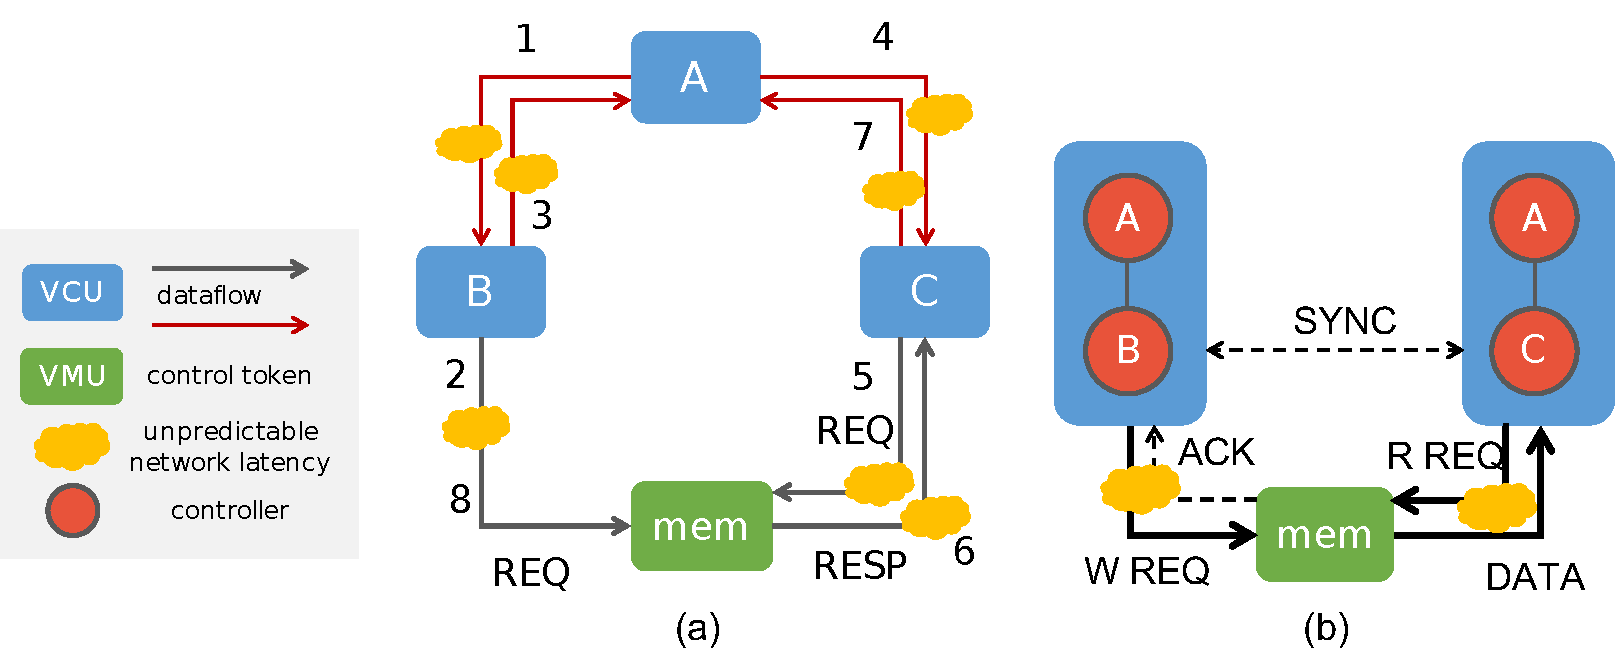
\includegraphics[width=0.8\textwidth]{figs/centralctrl.pdf}
\caption{
  (a) A na\"ive mapping strategy to map the control hierarchy onto Plasticine.
  All units are distributed across an on-chip network that can introduce unpredictable latency.
  The number on the edges indicate the order of event.
  Here we show a scenario where read requests from \emph{C} do not observe the write requests from
  \emph{B} that appears earlier in the program order due to network latency between \emph{B} and
  \emph{mem}.
  (b) Distributed controllers in \name. Each innermost controller makes a copy of all enclosing
  controllers. The signals from these controller are used to generate synchronization between
  distributed compute unit. To address the problem in (a), the memory also needs to provide an write
  acknowledgment per write request for synchronization.
}
\label{fig:centralctrl}
\end{figure*}

To achieve the same execution schedule on Plasticine in a na\"ive approach, 
we can map each controller in the hierarchy into a PU
, sending control signals to schedule the next level 
controllers distributed in other PUs, as shown in \Cref{fig:centralctrl} (a).
This strategy suffers from the expensive network round-trip delays between the parent and child controllers.
To be scalable at a high clock frequency, Plasticine networks are pipelined at each switch,
introducing multiple cycles of network delay across PUs on the control path.
Therefore, the multi-cycle handshaking signal between the parent and the child can introduce significant pipeline bubbles
that undermines performance.
Additionally, this scheme creates a communication hotspot around the parent controller \emph{A} as
loop \emph{A} gets unrolled, which is devastating for a coarse-grained reconfigurable architecture
like Plasticine that has much less routing resource than a FPGA.
Furthermore, synchronizing the compute only is insufficient to ensure memory effects are observed by
the remotely distributed accessors, as shown in \Cref{fig:centralctrl} (a).

To address this challenge, we want to eliminate any of the centralized schedulers for the outer
controllers.
At high-level, \name achieves this by performing loop division for each outer controller, such that
all innermost controllers are perfectly nested, as shown in \Cref{fig:centralctrl} (b).
\name then allocates synchronization tokens across distributed innermost controllers.
All innermost controllers have their own copies of the outer controllers, which are used
to control when to send and consume the control tokens.
These control token ensures the execution order of the inner controllers is the same as if they are
scheduled by a centralized outer controller. Instead of synchronizing all inner controllers under an
outer controllers, \name only synchronizes the ones accessing the same memory, such as \emph{B} and
\emph{C} in \Cref{fig:spatialegpar}. This limits the synchronization among a small set of distributed nodes, 
making our design much more scalable.

The second challenge in this mapping process is that controllers in the spatial hierarchy
can consume arbitrary amount of compute and memory resources, exceeding the capacity of individual
PUs. For instance, a user might write a memory multiple times throughput the program with writers 
mapped to different PUs. The physical scratchpad, however, only has a single write
port. \name needs to virtualize resources, composing or time sharing them when software usage
exceeding the hardware limit.

\begin{figure*}
\centering
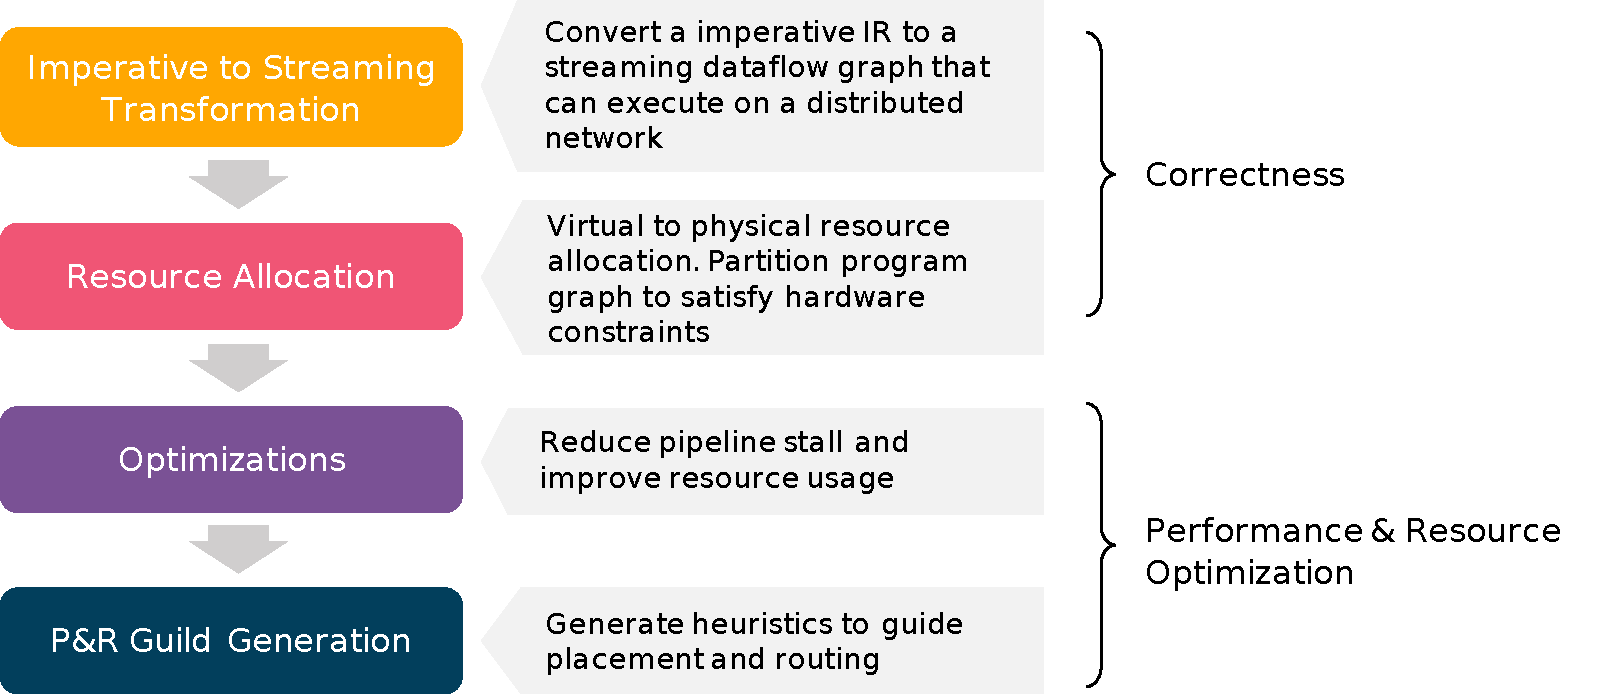
\includegraphics[width=1\textwidth]{figs/sarastack.pdf}
\caption[\name Compiler Flow]{\name Compiler Flow}
\label{fig:flow}
\end{figure*}
 
In the following sections, we describe a systematic approach to compile applications described in an
imperative front-end language to a purely declarative and distributed dataflow graph that can
run on Plasticine. \Cref{fig:flow} shows \name's compilation flow.

\Cref{sec:control} expands on the \term{imperative to streaming transformation} that
addresses the first challenge.
\name allocates distributed on-chip resources to execute the program in spatially parallelized and
pipelined fashion with approperate synchronizations.
A virtual unit (VU) is our intermediate representation that captures computations 
%that will be
%mapped onto 
within the boundary of
a physical unit (PU), such as a PCU and PMU.
Each VU can contain multiple contexts, if their aggregated resources usage can fit in a PU.
The hardware can limit the maximum number of contexts a PU can support and has resources that cannot be split across contexts.
Most importantly, \name needs to ensure messages across VUs, which are mapped across the global network, must tolerate an arbitrary amount of network latencies; messages within a single VU across contexts takes only a single cycle.
The transformation phase generates a virtual unit dataflow graph (VUDFG) with appropriate
synchronizations, such that a streaming pipelined execution over distributed on-chip resources produces the same result as a
parallelized program executed in time.
At the end of the allocation phase, a virtual unit can consume as much resources as the program
requires. 

\name further virtualizes resource allocation and hides the underlying resource constrains on
this hierarchical architecture from the programmers.
\Cref{sec:resalloc} dives into the \term{resource allocation} phase, where \name assign each VU to a
PU that processes the required resources. If no PU can execute a VU, \name partitions the
VU into multiple VUs to eliminate constraint violations. If there is insufficient PU or the VU cannot be partitioned, the mapping process fails with appropriate hints to the programmer for the
limiting resources.

Throughout the first two phases, \name introduces various \term{optimizations} that either reduce the
resource cost of the VUDFG, or alleviates potential performance bottleneck in the streaming
pipeline.
After all VU fits in at least one type of PU, \name performs a global optimization that merges small VUs into a larger VU to reduce resource fragmentations.
\Cref{sec:opt} enumerates the optimizations \name perform.

The output of the resource allocation phase is a VUDFG with a tagged PU type for each VU.
It is up to the
\term{placement and routing (PaR)} phase to determine where the VU will be finally placed.
Right before PaR, \name performs static analysis on the traffic pattern and generate heuristic guild
for the placer to reduce routing congestion.
\Cref{sec:par} details the PaR algorithm and heuristic-guild generated by \name.


\section{Distributed Control Flow}
\label{sec:control}

The input to \name is the backend of the Spatial IR, which is an control hierarchy after loop
unrolling.
The controller at each level of the hierarchy corresponds to a control primitive, such as a loop, or
a branch statement. A basic block is attached to each \emph{inner most} controller including instructions
and memory accesses to user declared data-structures.
\Cref{fig:spatialir} shows an example of a program and a schematic Spatial output IR.

\begin{figure*}
\centering
\begin{subfigure}[b]{0.4\textwidth}
\inputminted{python}{code/spatialeg.py}
\caption{Pseudo Spatial Example}
\end{subfigure}
\hfill
\begin{subfigure}[b]{0.58\textwidth}
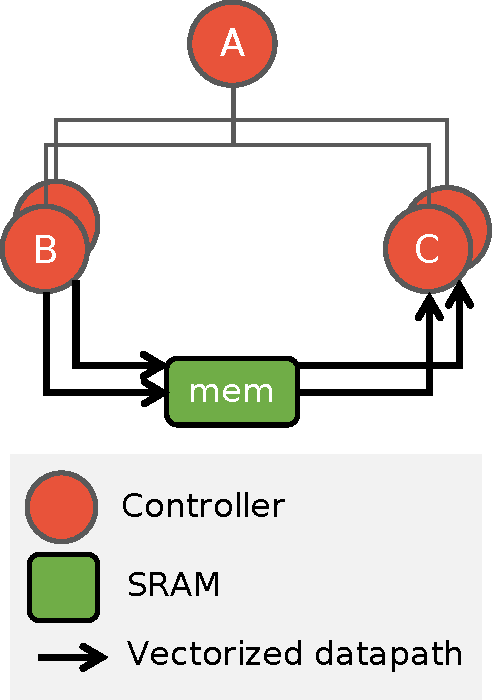
\includegraphics[width=1\textwidth]{figs/spatialir.pdf}
%\missingfigure[figwidth=1\textwidth]{Spatial IR}
\caption{Schematic Spatial IR}
\label{fig:spatialir}
\end{subfigure}
\caption[Spatial Example]{Pseudo example of \name's front-end language}
\end{figure*}

\begin{figure*}
\centering
%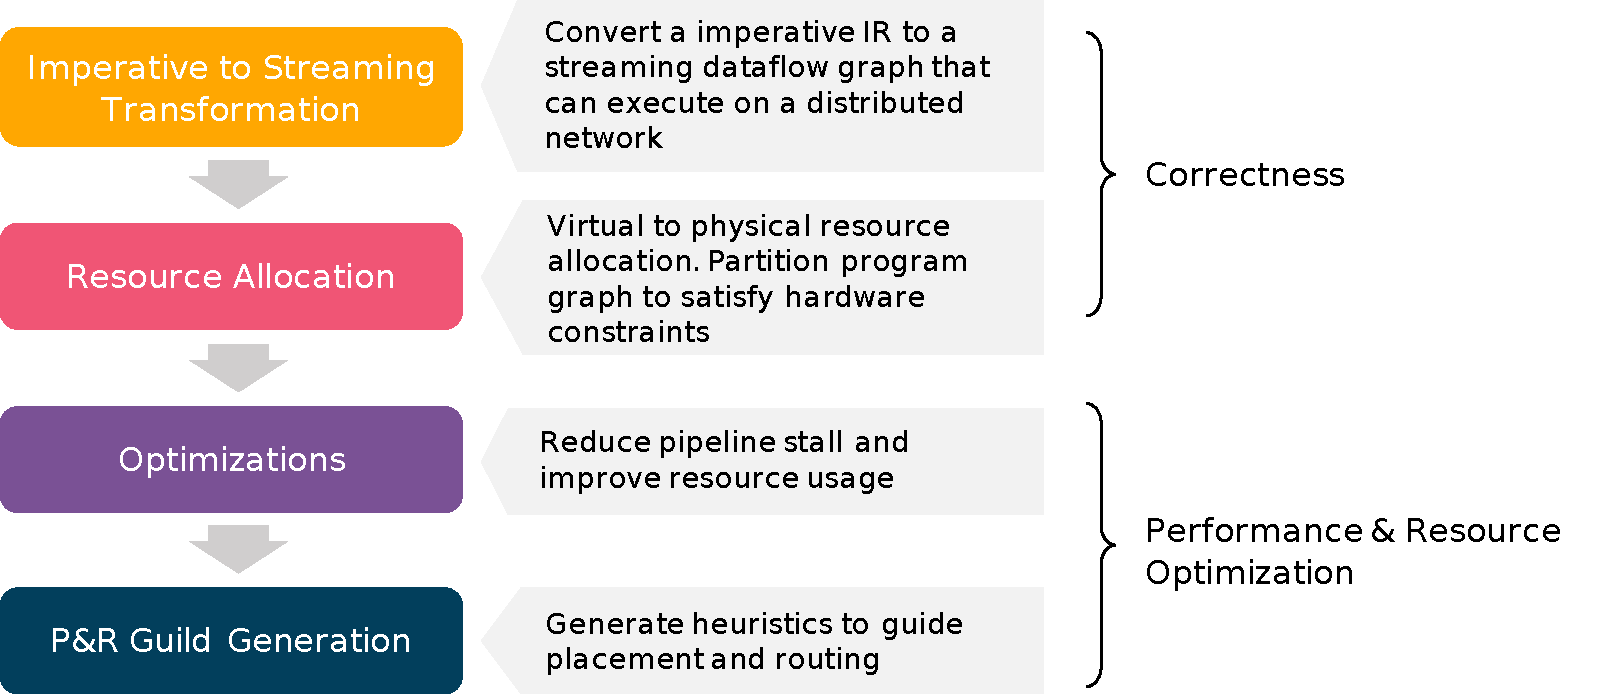
\includegraphics[width=1\textwidth]{figs/sarastack.pdf}
\missingfigure[figwidth=1\textwidth]{Controller duplication}
\caption[Context allocation]{Context allocation}
\label{fig:contextalloc}
\end{figure*}

%\begin{figure*}
%\centering
%\caption[Spatial IR]{Spatial IR}
%\label{fig:spatialir}
%\end{figure*}

As a start, \name allocates one virtual memory to hold each on-chip data structure, and 
one context to execute each basic block within the inner most controllers. 
A basic block maps naturally to a context, as instructions within a basic block are control-free. 
Next, \name makes a copy of all controllers enclosing the basic block in the corresponding context, as
shown in \Cref{fig:contextalloc};
these controllers are later converted to counters and control configurations supported by the
hardware. 
With these controllers, contexts can repeat execution for expected number iterations. However,
data-structures written and read by different contexts are accessed in random order.
The insight is that \emph{as long as all contexts accessing a shared memory with expected program order,
the final result is identical to a sequentially executed program}.
Unlike traditional out-of-order execution, where hardware and compiler look for independent instructions to
execute concurrently, \name starts with all basic blocks executing in concurrent contexts.
\name then introduces synchronizations to maintain consistent access order as expected by the 
program \emph{only} among contexts accessing a shared memory. 
This way, \name introduces minimum p2p synchronizations among small groups of contexts; contexts
accessing different memories are naturally parallelized without impacting the final output.
\todo{walk through an example here}.

To order the execution order or two contexts, \name allocates a single-bit \term{control token} as 
an access grant to the shared memory and passes it between contexts. 
This control token is no different from a regular data-dependency.
By controlling {\em where}, {\em how}, and {\em when} to pass the token, \name 
is able to maintain a consistent update ordering between the pipelined and parallelized actors that access the shared memory.

%In a na\"ive approach, we can map each controller in the hierarchy into a VB (\Cref{fig:centralctrl}).
%This strategy suffers from expensive network round-trip delays between the parent and child controllers.
%If the parent controller is an unrolled loop, the parent needs to synchronize with all child controllers, which creates an undesired communication hot spot.
%\Cref{fig:centralctrl}(a) shows an example where synchronization {\em just} between parent and child controllers can produce an incorrect result due to unpredictable network latency.

%The alternative approach explores a different way to execute the expected control schedule correctly. 
%The minimum required synchronization to produce the correct result is to ensure that the computations access the intermediate results in a consistent matter as if the control schedule is strictly enforced. 
%This can be achieved via p2p synchronizations \emph{only} between computations that access a particular shared memory.
%The execution order of computations that access different memories does not need to be enforced, as they do not impact the program outcome.
%Therefore, as long as the compututation is executed with the expected number of iterations and the memories are updated consistently, there is no need for any extra synchronization.
%Next, we walk through how \name{} achieves this in more concrete detail.


\subsection{Synchronization} 
\label{sec:sync}
We refer to an access to the memory in the input graph as a \emph{declared access}, as supposed to accesses executed at runtime.
For example, multiple accesses across loop iterations are counted as a single declared access.

\paragraph{Where.}
\name only allocate resource to synchronize actors if their declared accesses can potentially interfere.
Whether two declared accesses interfere depends on the type of accesses, the type of the memory, and location of the accesses in the control hierarchy.
For every declared access, \name{} checks other accesses of the same memory appeared earlier in the program order for a possible forward dependency, and later in the program order for a possible loop-carried dependency (LCD). 
Two declared accesses A and B have no dependency if their least-common ancestor (LCA) controller executes only one of the children at anytime (from a branch), or all children in parallel (from an unrolled loop).
The LCD exists between B to A, if B occurs later in the program order, and A and B are surrounded by a loop.
To detect LCD, \name checks if a loop exists among two accesses' LCA controller and LCA's ancestor controllers.
For a dual-ported SRAM, all other accesses need to be synchronized to: share address ports for read-after-read (RAR) and write-after-write (WAW); 
enforce true data-dependency for read-after-write (RAW); and
prevent the overriding of read data for write-after-read (WAR).
\gist{If the memory is multi-buffered (by the user or high-level compiler), we do not need to synchronize for WAR~\cite{dhdl} (the writer writes to a different buffer than the reader does). }
The DRAM interface permits concurrent read streams and, hence, RAR does not need to be synchronized.

\begin{figure*}
\centering
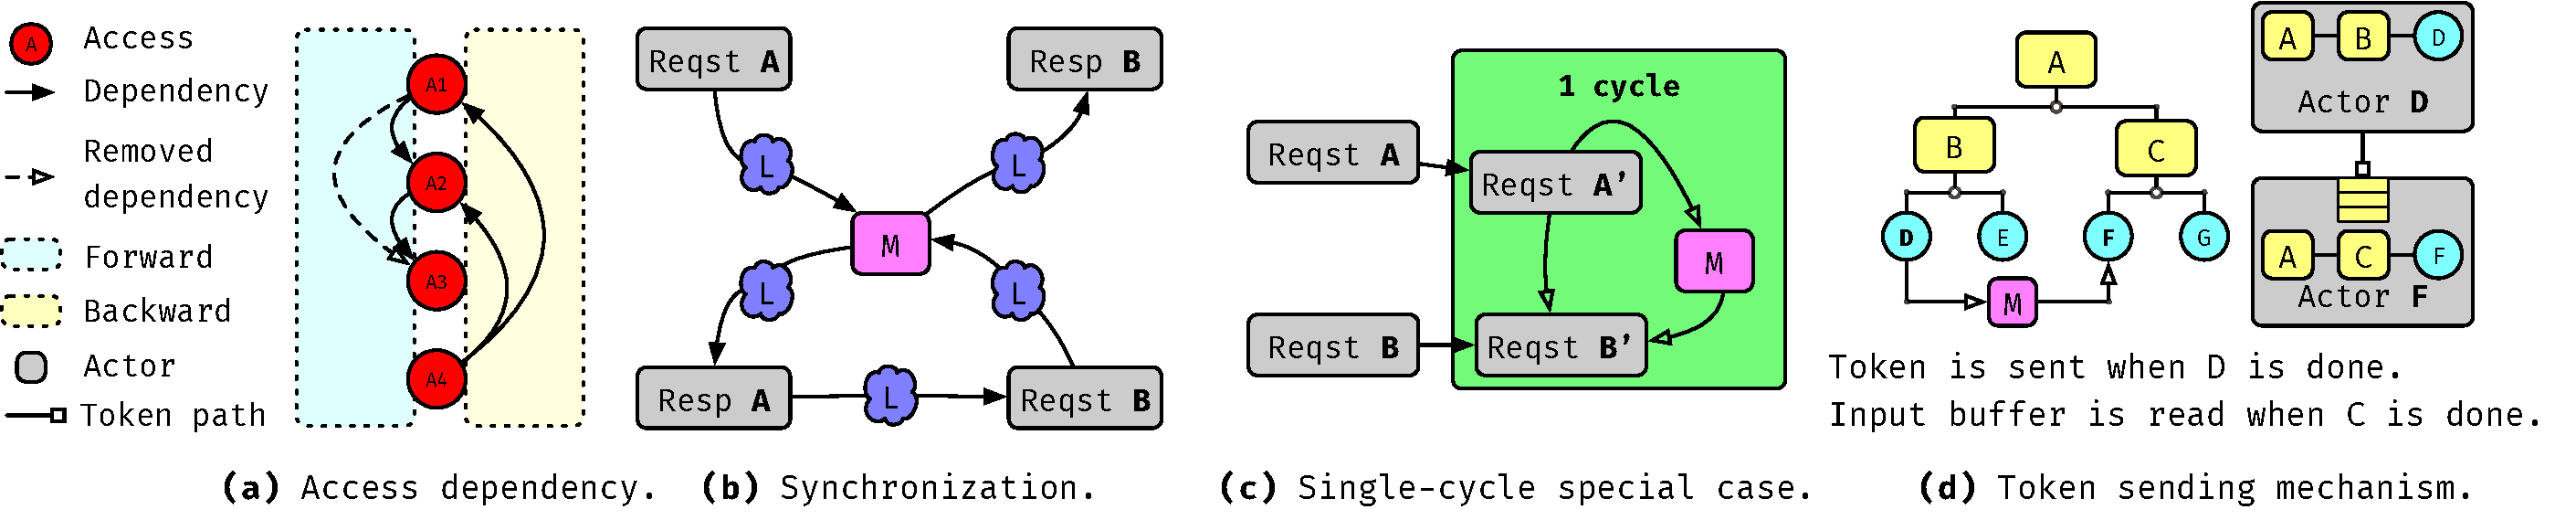
\includegraphics[width=1.0\textwidth]{figs/synch_mech.pdf}
\caption{
    (a) Access dependency graph.
    (b) Synchronization of two accesses on the same memory.
    (c) Single-cycle special case.
    (d) Actors uses local states of controller hierarchy to determine when to send a token.
}\label{fig:depgraph}\label{fig:token}\label{fig:tokentrick}\label{fig:tokenwhen}
\end{figure*}
%\ms{repeated caption, rather give a single caption.}

\paragraph{How.} For each intermediate memory, \name{} builds a dependency graph for all its declared accesses (\Cref{fig:depgraph}(a)).
Enforcing all dependencies in this graph may not be necessary as dependencies between $A_1$ and $A_2$, and $A_2$ and $A_3$ already capture the dependency between $A_1$ and $A_3$.
Therefore, \name{} performs a transitive reduction (TR) on the graph to keep the minimum number of dependency edges that preserve the same ordering \cite{tr}.
Since TR on a cyclic graph is NP-hard, we perform TRs on the forward and backward LCD graphs, separately.
Notice, dependencies between accesses touching different buffers of a multi-buffered memory is less rigid than accesses touching the same buffer.
Therefore, we can only remove an edge if all dependencies on the equivalent path have a stronger or equivalent dependency strength than the strength of the removed edge.

To eliminate the round-trip overhead between the memory and the computation, 
\name{} duplicates the local states and expressions required to generate the requests in a separate actor as the one that handles the responses.
For write accesses, the memory provides an acknowledgment for each request received, used by \name for synchronization.
The request actor generates requests asynchronously as soon as its data-dependencies are cleared, pushing all requests to memory until back-pressured.
To order a declared access A before a declared access B
\name creates a dummy dependency between the actor that accumulates the response of access A ($resp_A$) and the actor that generates requests for access B ($reqst_B$) (\Cref{fig:token}(b)).
To enforce LCD from access B to access A, \name introduces a token from $resp_B$ to $reqst_A$, and initializes the token buffer (input buffer receiving the token) with one element to enable the execution of the first iteration.
If the LCD is on a multi-buffered memory, the LCD token is initialized with the buffer depth number of elements to enable A for multiple iterations before blocked by access B.

These are general schemes we use on any types of memory (including DRAM and on-chip memories) with unpredictable access latency.

\subparagraph{Special Case: Single-Cycle Access}
For a memory with guaranteed {\em single-cycle} access latency, such as registers and statically banked SRAMs that are guaranteed conflict-free, we can simplify the necessary synchronization (\Cref{fig:tokentrick}(c)).
Instead of synchronizing between $resp_A$ and $reqst_B$, we allocate two stateless actors $reqst_A'$ and $reqst_B'$ within {\emph the same} VB as the accessed memory that forwards requests from $reqst_A$ and $reqst_B$, respectively.
Next, we forward the token going from $reqst_A$ to $reqst_B$ to go through $reqst_A'$ to $reqst_B'$ instead, and configure the token buffer in $reqst_B'$ with the depth of one for serialized schedule and depth of M for multi-buffered schedule. 
We no longer need to insert the LCD token, as the stiff back pressure from the token buffer in $reqst_B'$ will enforce the expected behavior.
This optimization only works if the sender and receiver of the token buffer are physically in a single VB where the memory is located.
In this way, when $reqst_B'$ observes $reqst_A'$s token, $reqst_B'$ is guaranteed to observe the memory update from $reqst_A'$ because the memory also has single-cycle access latency.

\subparagraph{Memory Localization}
We perform another specialization on non-indexable memories (registers or FIFOs), whose all accesses have no explicit read enables.
Instead of treating them as shared memories, \name{} duplicates and maps them to local input buffers in all receivers, no longer requiring tokens.
The sender actor pushes to the network when the token is supposed to be sent, and the receiver dequeues one element from the input buffer when the token is supposed to be consumed.
This dramatically reduces the synchronization complexity of non-indexable memory in the common case.

\paragraph{When.}
\name{} configures the actors to generate the token using their local states at runtime.
For FIFOs, the token is generated and consumed every cycle when the producer and receiver actors are active.
For register, SRAM, and DRAM the program order expects that the producer and consumer writes and inspects the memory once per iteration of their LCA controller, respectively.
Since the producer and receiver both have their outer controllers duplicated in their local state, they have independent views for one iteration of the LCA controller, which is when the controller in their ancestors (that is the immediate child of the LCA controller) is completed (\Cref{fig:tokenwhen}(d)).
The {\em done} signals of these controllers are used to produce and consume the token in actors, independently.

\subsection{Data-Dependent Control Flow}
Using the synchronization discussed in \Cref{sec:sync}, we can support control constructs that typically are not supported on most RDAs, such as branch and a while convergence loop.
The controllers in the input graph can also have data dependencies, such as loop ranges. 
The dynamic-loop ranges are handled as data dependencies to actors with \emph{memory localization} described in \Cref{sec:sync}.
The branch condition is also treated as a data-dependent enable signal of controllers under branch clauses.
If the controller is disabled, it is considered {\em done} immediately.
Output tokens depending on the {\em done} signal will be immediately sent out.
For a memory written inside a branch statement and read outside the branch (with a branch miss), the writer actor immediately sends out the token to the receiver
as soon as the branch condition is resolved. 
With a branch hit, the controller waits until its inner controller completes before raising the {\em done} signal.
%This way, the 
A similar scheme is used to implement the while loop, where the while condition is a data-dependency of stop signal of controller X. 
The producer of the while condition also consumes its own output as an LCD. 
The condition is then broadcast to all other actors under the same while loop. 
The {\em done} signal of the while loop is raised when the condition's data-dependency evaluates to true.
At this point, actors accessing memory within the while loop will send the token to access actors outside of the while loop, and enable them to access the intermediate memory.

After all actors and shared resources are allocated and synchronized, we simply put each actor and shared resource into their own VBs.
The actors with single-cycle special case (\Cref{sec:sync}) must be put in the same VB as the shared memory.


\section{Resource Allocation} \label{sec:resalloc}

The output of the imperative to dataflow transformation discussed in \Cref{sec:control} is a VUDFG that 
can execute on a Plasticine with physical units (PUs) that have infinite resources.
The \emph{Resource Allocation} phase enforces and addresses constraint violations given 
the specification of the Plasticine units. 
At the end of this phase, \name assigns each VU in the VUDFG graph to a PU type with required
resources; the placer then takes the type assignments and determines the final placement.

Accelerators often have heterogeneity in compute resources to improve efficiency for common
special operations.
In Plasticine, PMUs and AGs have specialized compute pipelines for address calculation that are 
less capable than the compute pipeline in PCUs.
However, heterogeneity tends to reduce average utilization because different applications, and even the same application with different data sizes, can vary highly in the desired ratio among different
resource~\cite{tz_rnn}.
A compute-bound application, for example, can heavily underutilize the AGs and PMUs.
To address this problem, \name models the virtual to physical assignment as a constraint satisfaction problem; 
each VU consumes a set of resources and can only be assigned to a PU if the PU processes the required resources. 
%Instead of using heuristics to assign certain a type of VU to a type of PU, we
\Cref{tab:resource} shows the types of resources \name models in Plasticine's heterogeneous units.
For example, special connection to off-chip memory interface is
also treated as a type of resource in the AG, which forces virtual contexts accessing DRAM to map to AGs. 
On the other side, regular contexts with non-vectorized fixed-point operations can also be mapped to
spare AGs, which improves utilization.
\begin{table*}
  \centering
\begin{tabular}{lccccc}
  \toprule
  Feature & PCU & PMU & AG & Host Unit & Aggregation Function\\ \midrule
  Vector lane width & 16 & 16 & 1 & 1 & \multirow{2}{*}{MAX}\\
  \# pipeline register (PR) & 8 & 8 & 4 & 0 & \\ \hline
  \# stages & 6 & 10 & 5 & 0 & \multirow{6}{*}{SUM}\\
  Scratchpad banks & 0 & 16 & 0 & 0 &  \\
  Scratchpad capacity & 0 & 256kB & 0 & 0 & \\
  MergeBuffer & 1 & 0 & 0 & 0 & \\
  Splitter & 1 & 0 & 0 & 0 & \\
  Scanner & 1 & 0 & 0 & 0 & \\ \hline
  Operation types & fix $\cup$ float & fix & fix & $\varnothing$ & $\cup$ \\ \hline
  Reduction tree & \cmark & \xmark & \xmark & \xmark & \multirow{3}{*}{OR}\\
  Access to DRAM Interface & \xmark & \xmark & \cmark & \xmark & \\
  Access to Host IO & \xmark & \xmark & \xmark & \cmark & \\ \hline
  \# Vector Input & 6 & 6 & 4 & 0 & \multirow{6}{*}{G}\\
  \# Scalar Inputs & 6 & 6 & 4 & 16 & \\
  \# Control Inputs & 16 & 16 & 4 & 16& \\
  \# Vector Outputs & 6 & 6 & 4 & 0 & \\
  \# Scalar Outputs & 6 & 6 & 4 & 16 & \\
  \# Control Outputs & 8 & 8 & 2 & 16 & \\
 \bottomrule
\end{tabular}
\caption[Resources specification of heterogeneous units and aggregation function]{
  A list of resources \name models in four types of configurable units in Plasticine. The host unit
  models the host registers I/Os.
  MergeBuffer, Splitter, and Scanner are new hardware units introduced in \cite{gorgon} and recent work
  to support database and sparsity in Plasticine.
  The aggregation function indicates how to compute the aggregated resource cost when two contexts are merged
  into a single virtual unit (VU). G indicates the aggreated value is the output of a graph traversal of the
  merged graph. How to count \# I/O is discussed later in \Cref{sec:compsplit}.
  While the aggreation function of \#PR of two merged contexts is MAX, the \#PR of a
  context is the maximum number of live variables of its dataflow graph, which is also an output of
  a topological traversal.
  This table reflects a different Plasticine configuration as the original Plasticine in \cite{plasticine}.
}
\label{tab:resource}
\end{table*}

\begin{algorithm}
  \Fn(\tcc*[h]{Allocation Algorithm}){alloc(V, P, pruners)}{
    \KwData{V: a set of VUs from the VUDFG}
    \KwData{P: a set of all PUs on the hardware}
    \KwData{pruners: a list of constraint pruners to check
    and fixes constraint violations}
    \tcc{Initialize a complete bipartite graph}
    G = \KwNew BipartiteGraph()\;
    G[V] = P\;
    \tcc{Constraint resolution}
    prune(G, pruners)\;
    \tcc{Global merging}
    merge(G)\;
    \tcc{Heuristic check on whether assigning all VUs in V is feasible}
    check(G)\;
    \tcc{Virtual to physical assignment}
    backtracking\_assign(G)\;
  }
  \vspace{0.5cm}
  \Fn(\tcc*[h]{A recursive pruning function}){prune(G, pruners)}{
    \KwData{G: bipartite graph between VUs and PUs}
    \KwData{pruners: a list of constraint pruners to check
    and fixes constraint violations}
    \KwResult{The function update G by removing VU-PU edges that violates constraints guarded by
    pruners. The function may fail and raise an exception.}
    \tcc{All PUs on the hardware}
    P = G.values()\;
    \For{pruner \KwTo pruners}{
      \For{v \KwTo G.keys()}{
        \For{p \KwTo G[v]} {
          \If{pruner.cost(v) > pruner.cost(p)} {
            G[v] -= p\;
          }
        }
        \If{G[v].empty()} {
          \tcc{Partition VU v based on resource constraints registered in pruner. 
          Not all resources can be partitioned and this step may fail.
          If succeeded, the function returns a new set of VUs.}
          V' = pruner.partition(v)\;
          G' = \KwNew BipartiteGraph()\;
          G'[V'] = P\;
          prune(G',pruners)\;
          G -= v\;
          G[V'] = G'[V']\;
        }
      }
    }
  }
  \caption{Resource allocation. The bipartite graph \texttt{G} contains a bi-directional many-to-many
  map. \texttt{G[key]} returns the set of values connecting to the key (dom(key)), and \texttt{G[value]}
  returns the set of keys connecting to the value.
  \texttt{G[key] = value} connects an edge between key and value.
  \texttt{G[KeySet] = ValueSet} creates all-to-all connection between \texttt{KeySet} and
  \texttt{ValueSet}.}
  \label{algo:resalloc}
\end{algorithm}

\begin{algorithm}
  \Fn(\tcc*[h]{Assignment feasibility check}){check(G)}{
    \KwData{G: bipartite graph}
    \KwResult{Whether it is possible to assign all VUs in V with a different PU in P}
    \tcc{For every value set in \texttt{G}}
    \For{V \KwTo G.values().toSet()} {
      K = $\varnothing$\;
      \For{v \KwTo V} {
        \For{k \KwTo G[v]} {
          \If{G[k] $\subset$ V} {
            K += k\;
          }
        }
      }
      \If{|K| > |V|} {
        \KwRet{failure()}\;
      }
    }
    \KwRet{success()}\;
  }
  \caption{Heuristic check on whether it is possible to assign all key with an value in a bipartite
  graph. Given there are only a few types of hardware tiles, $G.values().toSet()$ is
  relatively small. This algorithm roughly runs in $O(|G.keys()|\times|G.values()|)$, which is
  still much faster than the backtracking assignment with exponential runtime.}
  \label{algo:check}
\end{algorithm}
 
%% backtracking_assignment(vu, dom)
As shown in \Cref{algo:resalloc}, the \emph{resource allocation} phase contains three steps:
\emph{constraint resolution}, \emph{global merging}, and \emph{virtual to physical assignment}.
\name uses a VU-PU bipartite graph (\emph{G}) to keep track of potential valid assignments between the two.
Initially, \emph{G} is initialized to a complete bipartite graph, i.e., all VUs can be assigned to
all PUs.
We refer to all PUs connected to a VU \emph{v} as the domain of \emph{v} in G, i.e. \emph{dom(v)}.

\paragraph{Constraint Resolution}
A list of constraint pruners, each considering a set of on-chip resources, 
incrementally remove the VU-PU edges that violate the resource constraints.
If a VU \emph{v} has an empty domain after pruning, the pruner attempts to fix the violation by
decomposing the VU into multiple VUs. 
Not all resources are composable, and the partitioning transformation may fail.
If succeeded, the partitioner generates a new set of VUs \emph{V'}. \name starts a new complete bipartite
graph between \emph{V'} and all resources \emph{P}, and recursively prune on \emph{V'}.
If succeeded, the original graph \emph{G} is updated with \emph{V'} and their pruned resources.

\paragraph{Global Merging}
After all VUs have at least one PU in the bipartite graph, \name triggers a global optimization that merges 
small VUs into a larger VU to reduce fragmentation in allocation.
Each type of resource has an aggregation rule to compute how the resource cost changes if two VUs are merged
together, as shown in \Cref{tab:resource}. 
Most aggregation rules are simple, such as addition, logical or, max, or union.
The in- and out-degree costs are tricker and will be detailed in \Cref{sec:compsplit}.

\paragraph{Virtual to Physical Assignment}
Next, \name performs a quick heuristic check on the bipartite graph to see if there exists a
possible assignment for all VUs with sufficient PUs (\Cref{algo:check}), and provide feedback on the limiting resources, otherwise.
Finally, \name assigns each VU to a PU type with a backtracking search on the pruned bipartite
graph.

This approach can be easily extended to handle new heterogeneous tiles in the architecture by registering
the tile with existing or new types of resources with aggregation and partitioning rules.
The rest of this section goes over two types of partitioning transformations--compute
partitioning in \Cref{sec:compsplit} and memory partitioning in \Cref{sec:memsplit}.
%We have another partitioner encoding valid rule to decompose a BlackBox IP block available on the RDA.

\subsection{Compute Partitioning} 
\label{sec:compsplit}

The {\em compute-partitioning} phase addresses VUs using more compute resources than any PU can provide. 
If a VU contains multiple contexts, \name{} first moves the contexts into separate VUs.
If a single context exceeds the resource limit, \name breaks down the dataflow graph in the context into multiple contexts and puts them in separate VUs.
During partitioning, \name maps each subgraph of the large dataflow graph into a new context, mirrors the control states of the original context, and streams live variables in between.
We can formulate the problem of how to partition in the dataflow graph as an optimization problem, shown in
\Cref{tab:partprob}.
The partitioner ``fixes'' the VU \emph{v} based on a single PU specification, albeit there are many potential PUs 
the decomposed VU can be mapped to.
Currently, we use a heuristic to select a PU type from \emph{dom(v)} right before the compute pruning 
as a guiding constraint for partitioning.

\begin{table*}
  \centering
\begin{tabular}{lp{12cm}}
  \toprule
  \textbf{Problem} & Partition the dataflow graph into subgraphs such that all subgraphs satisfy the constraints of a
  hardware unit. \\[0.9cm]
  \textbf{Objective }& Minimize the number of partitions and connectivity across partitions. \\[0.5cm]
  \textbf{Constraints} & 
  \begin{minipage}{12cm}
  \begin{outline}
  \0 Each partition must not exceeds the limit on the number of \vspace{-0.2cm}
    \1 live in/out variables (I/O ports) \vspace{-0.2cm}
    \1 operations (pipeline stages), \vspace{-0.2cm}
    \1 and live variables across operations (pipeline registers), etc.\vspace{-0.2cm}
  \0 No \emph{new} cycles can form across partitions other than the cycles in the original
  dataflow graph.
  \end{outline}
  \end{minipage}
  \\
 \bottomrule
\end{tabular}
\caption[Formulation of the compute partitioning problem]{
Formulation of the compute partitioning problem
}
\label{tab:partprob}
\end{table*}

Because the global network is specialized to handle efficient broadcasts, 
the in/out-degree of a partition counts the number of unique live-in/out variables, as supposed to
the number of edges across partitions.
In addition, the partitioned subgraphs cannot form {\em new} cycles; contexts waits for all
input dependencies and therefore cycles across contexts cause deadlock. 
Nonetheless, the original graph might contain cycles representing loop-carried dependencies, such as
accumulation. For these cycles, \name initializes the back edge of the cycle with dummy data to
enable execution.
\Cref{fig:parteg} shows examples of valid and invalid partitioning solutions.
\Cref{fig:partcycleeg} shows another partitioning example of a dataflow graph with cycles.

\begin{figure}
  \centering
  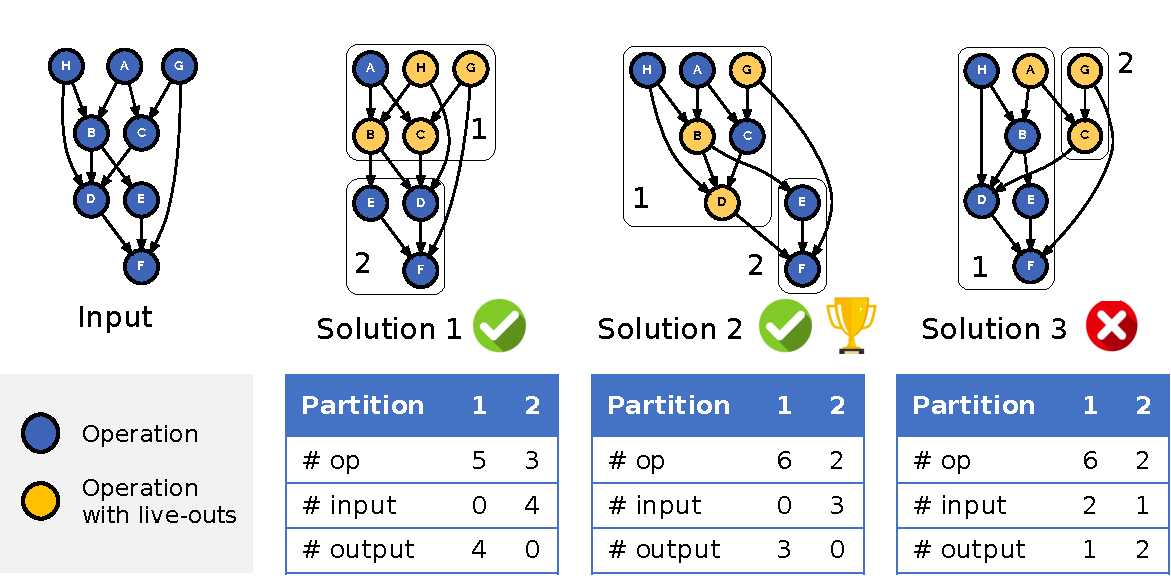
\includegraphics[width=1\columnwidth]{figs/parteg.pdf}
  \caption[Compute partitioning examples]{
    Compute partitioning examples. Solution 1 and 2 are both valid. Solution 2 is
    better because it has less number of broadcast edges across partitions (3 as supposed to 4 in Solution 1). 
    Solution 3 is an illegal partitioning due to the cycle between partition 1 and 2.
  }
  \label{fig:parteg}

  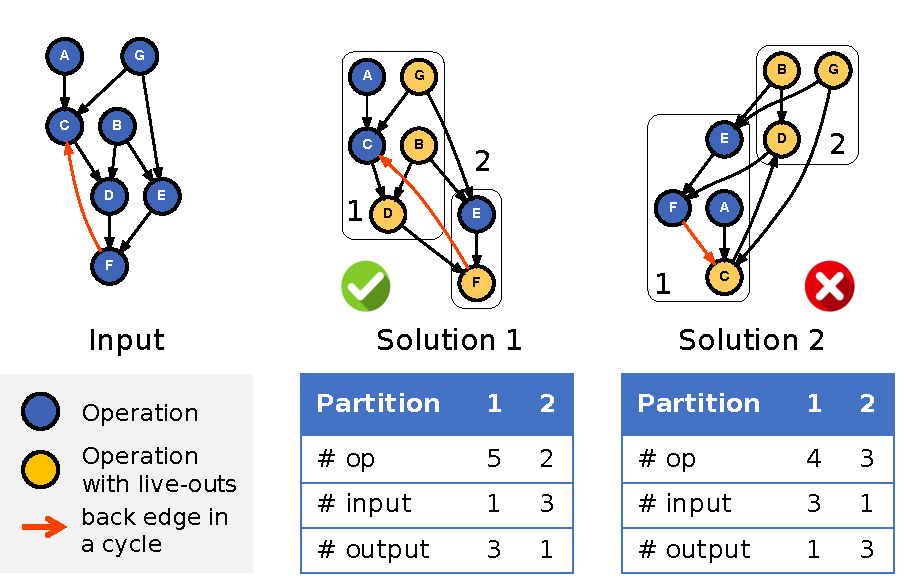
\includegraphics[width=0.8\columnwidth]{figs/partcycleeg.pdf}
  \caption[Compute partitioning examples with cycle]{
    Compute partitioning examples with cycle in the dataflow graph.
    Solution 1 is valid because there is no 
    cycle between partitions after removing the back edge in
    the original graph.
    Solution 2 is invalid because there is still cycle between partition 1 and 2 after
    removing the back edge.
  }
  \label{fig:partcycleeg}
\end{figure}

\paragraph{Community Detection}
The formulation of compute partitioning is similar to the community detection
problem\cite{community} that has a similar objective. 
The major difference is that the latter often takes the number of output partitions as an
input to the algorithm, whereas our problem partitions until all subgraphs satisfy all constraints.
Moreover, community detection algorithms do not enforce the cycle constraints. 
Finally, the edge connectivity in community detection counts the number of edges across partitions, 
as supposed to broadcast edges as in our problem.

\paragraph{Retiming}
Imbalanced data paths across partitions can cause pipeline stalls at runtime if the long-live path is not
sufficiently buffered.
To ensure full-throughput pipelining, \name needs to insert retiming buffers along the imbalanced data path across
partitions.
Retiming introduces new VUs in addition to the partitioned VUs, which attributes to the cost in
\Cref{tab:partprob}'s objective.

In the following sections, we present two algorithms to resolve the problem described in
\Cref{tab:partprob}:
a fast traversal-based algorithm providing a decent solution, and a slow convex
optimization-based algorithm providing an optimal solution.

\subsubsection{Traversal-based Solution}
To address the cycle constraint, the traversal-based algorithm performs a topological sort of the dataflow graph.
The topological sort ignores the back edges of the cycles during traversal. 
Starting from one end of the sorted list, the algorithm iteratively adds nodes into a partition
until it fits no more nodes. The algorithm then repeats the process with a new partition.
This approach guarantees that no cycle is introduced with $O(V+E)$ complexity, 
where $V$ and $E$ are the numbers of vertices and edges in the dataflow graph.

The partitioning result is a function of the traversal order.
We experienced with depth-first search (DFS) and breadth-first search (BFS) with forward and
backward dataflow traversal orders.
For DFS, we re-sort the remaining list each time starting with a new partition.

\subsubsection{Solver-based Solution}
The convex optimization solution models the problem as a node-to-partition assignment problem.
\Cref{tab:solver-eqns} gives our formulation and \Cref{tab:solver-variables} explains the notations
used in \Cref{tab:solver-eqns}.

\begin{table*}
  \centering
	\begin{tabular}{c | c | c | c}
		\textbf{Name} & \textbf{Type} & \textbf{Description} & \textbf{Definition / Default}\\\hline
		$\mathcal{N}$ & Constant & Enumeration of nodes to partition, numbered $\{n_i\}_i$ & - \\
		N & Constant, $\nnint$ & Number of operations to partition & $N = |\mathcal{N}|$\\
		P & Constant, $\nnint$ & Number of partitions to consider & $N$, or from heuristic \\
		$\mathcal{E}$ & Constant, $\{n_i \to n_j\}$& Directed edges representing dependence & - \\
		B & Variable, $\{0, 1\}^{N \times P}$ & Boolean Partitioning Matrix& - \\
		%p & Variable, $\nnint^N$ & Vector of mappings from node to assigned partition& $p = B \begin{bmatrix} 0 & 1 & \cdots & P-1\end{bmatrix}^T$\\
		$\projb{\cdot}$ & $\nnint \to \mathbb{B}$ & Function to convert a positive integer into a boolean& Supplemental Materials\\
		$\andf(\cdot, \cdot)$ & $\{0, 1\} \times \{0, 1\} \to \{0, 1\}$ & Boolean and of binary variables & Supplemental Materials \\ 
		$d_p$ & Variable, $\nnint^P$ & Vector of partition delays & - \\
		$d_n$ & Variable, $\nnint^N$ & Vector of node delays & - \\
		$\dest(n)$ & $\mathcal{N} \to \mathcal{P}(\mathcal{N})$& The set of nodes which depend on $n$& $\{n' | n' \in \mathcal{N}\ s.t.\ (n \to n') \in \mathcal{E}\}$\\
		$c_o$ & Constant, $\nnint$ & Maximum output arity of a partition & HW Spec \\
		$c_i$ & Constant, $\nnint$ & Maximum input arity of a partition & HW Spec \\
		$b_d$ & Constant, $\nnint$ & Maximum input buffer depth & HW Spec \\
		$K$ & Constant, $\mathbb{R}_+$ & Very Large Constant, used for constraint activation & $P \times N$ \\
		$\alpha_d$ & Hyperparameter, $\mathbb{R}_+$ & Retime merging probability multiplier& $\frac{1}{\max\{c_o, c_i\}}$ \\
	\end{tabular}
	\caption{Names and definitions used in the solver-based partitioning.}
	\label{tab:solver-variables}
\end{table*}

\begin{table*}
  \centering
  \newcommand\cola{1.6cm}
  \newcommand\colb{3.8cm}
  \newcommand\colc{9cm}
  \newcommand{\gcell}[2]{\Gape[#1cm][0cm]{\makecell[l]{#2}}}
  \begin{tabularx}{\textwidth}{cp{\colb}X}
    \toprule
		\textbf{Type} & \textbf{Description} & \textbf{Expression}\\\midrule
    \multirow{3}{*}{\makecell[l]{Cost\\Function}} & Allocated Partitions & $\Sigma_i \projb{\Sigma_j B_{i, j}}$\\

    & \makecell[l]{Additional Retiming\\Partitions}
    & $\alpha_d \Sigma_{n_i \to n_j \in \mathcal{E}} \projb{\max\{d_n(j) - d_n(i) - b_d, 0\}}$\\[0.3cm]
		\hline

    \multirow{12}{\cola}{\makecell[l]{\\\\Constraint}} & Partition Assignment & $ \forall n_i \in \mathcal{N}:\ \Sigma_j B_{i, j} = 1$\\[0.1cm]

    &\makecell[l]{Dependency\\Constraint} & $\forall n_i \to n_j \in \mathcal{E}:\ d_n(i) + 1[p_i \ne p_j] \le d_n(j)$\\[0.1cm]

    &\makecell[l]{Output Arity\\ Constraint} 
    &\makecell[l]{
      $\forall p \in [0, P):$ \\
      $\Sigma_{n_s \in \mathcal{N}} \andf(B_{s, p}, \projb{\max\{(\Sigma_{n_d \in \dest(n_s)} B_{d, p}) -$ \\
      $K \times B_{s, p}, 0\}}) \le c_o$
    }\\[0.7cm]

    &\makecell[l]{Input Arity Constraint\\ (vectorized)} & $\Sigma_{n_i \in \mathcal{N}} \max\{\projb{\Sigma_{n_j \in \dest(n_i)} B_{j, :}} - B_{i, :}, 0\} \le c_i \times \vec{1}$\\

		&Delay Consistency& 
    \makecell[l]{
    $\forall n_i \in \mathcal{N}:\ d_n(i) \le \min_j (d_p(j) + K - B_{i, j} \times K)$ \\
		$\forall n_i \in \mathcal{N}:\ d_n(i) \ge \max_j (d_p(j) + B_{i, j} \times K - K)$
    }\\[0.5cm]

		&Constant Validity& 
    \makecell[l]{
      $\forall n_i \in \mathcal{N}:\ d_n(i) \le K$\\
		  $\forall i \in [0, P):\ d_p(i) \le K$
    } \\
    \bottomrule
	\end{tabularx}
  \caption{Solver formulation for partitioning*.}
	\label{tab:solver-eqns}
\end{table*}

\begin{table*}
	\begin{tabular}{c | c | c | c}
		\textbf{Name} & \textbf{Type} & \textbf{Description} & \textbf{Definition / Default}\\\hline
		$\mathcal{C}_r$& $[\mathcal{N} \to \mathbb{R}_+,\mathbb{R}_+, [\mathbb{R}_+] \to \mathbb{R}_+]$ & List of per-node values, limits, and reduction& Supplemental Materials\\&& functions for reducible constraints& \\
		F & $\{0, 1\}^{N \times P}$ & Feasibility matrix, whether a partition can support a node& HW Spec \\ 
	\end{tabular}
	\caption{\Cref{tab:solver-variables} extension for solver-based merging, which is a generalization of the partitioning problem.}
	\label{tab:merging-variables}

	\begin{tabular}{c | c | c}
		\textbf{Type} & \textbf{Description} & \textbf{Expression}\\\hline
		Constraint & Feasibility Constraint & $ \forall i, j \in [0, N) \times [0, P):\ B_{i, j} \le F_{i, j}$\\
		& Reducible Constraints & $\forall j \in [0, P).\ \forall (c(\cdot), c_v, r(\cdot)) \in \mathcal{C}:\ r([c(n_i) \times B_{i, j}]_{n_i \in \mathcal{N}}) \le c_v$\\
	\end{tabular}
  \caption{\Cref{tab:solver-eqns} extension for solver-based merging*. The Retiming Partition objective is not used for merging.}
	\label{tab:merge-eqns}
  \scriptsize
  \raggedright
  \vspace{-0.3cm}
  *Expressions are presented using the Disciplined Convex Programming ruleset \cite{DCP, DCP-online}. Explanations for selected expressions can be found in the supplemental material.
\end{table*}



At a high-level, we use a boolean matrix $B$ to keep track of the assignment. 
$B$ has dimension equals to the number of nodes in the dataflow graph by the maximum number of partitions, where$B[i,j]=1$ 
indicates node $i$ is assigned to partition $j$.
In \Cref{tab:solver-eqns}, \emph{partition assignment} restricts each node to have a single partition assignment.
The \emph{input and output arity constraints} show the formulations that limit the number of input
and output for a subgraph.
These are the two most challenging constraints as we need to identify broadcast edges across partitions.
To address the cycle constraint, we introduce a delay vector $d_n$ with a size equivalent to the number of nodes. 
The delay vector encodes a time schedule to execute each node, whose values are selected by the solver.
The \emph{dependency constraint} enforces a node can be scheduled no earlier than its input dependencies and
no later than its output dependents.
Since the operations within a partition have to be triggered atomically, there is another delay
vector $d_p$ for partitions. The \emph{delay consistency} enforces the schedule of a node equals to the
schedule of its assigned partition.
Finally, \emph{constant validity} limits the range of values the delay vectors can be chosen from.
In addition to enforcing the cycle constraint, 
these delay variables are also used to calculate where retiming is required and project the amount of introduced retiming VUs. 
Finally, we use the traversal-based solution to warm start the assignment matrix
$B$ and the delay vectors to reduce the solver runtime.

\subsubsection{Comparison}

\begin{figure*}
\centering
\hfill
\begin{subfigure}[b]{0.35\textwidth}
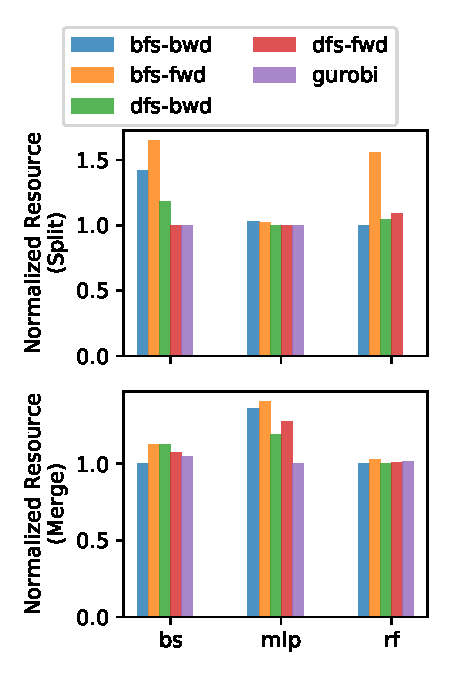
\includegraphics[width=1\textwidth]{figs/algo2.pdf}
\caption{Resource Comparison}
\end{subfigure}
\hfill
\begin{subfigure}[b]{0.64\textwidth}
\centering
\begin{tabular}{lccccc}
  \toprule
  Apps &bfs-bwd & bfs-fwd & dfs-bwd & dfs-fwd & gurobi \\ \midrule 
bs & 3s & 3s & 2s & 2s & 2h4m \\ 
mlp & <1s & <1s & <1s & <1s & 4s \\ 
rf & 1m37s & 1m7s & 29s & 27s & - \\ 

 \bottomrule
\end{tabular}
\caption{
  Compile time for spltting
}
\vspace{0.1cm}
\begin{tabular}{lccccc}
  \toprule
  Apps &bfs-bwd & bfs-fwd & dfs-bwd & dfs-fwd & gurobi \\ \midrule 
bs & 1s & 2s & 5s & 3s & 1m4s \\ 
mlp & 5s & 5s & 6s & 11s & 31m16s \\ 
rf & 11s & 10s & 2m7s & 1m0s & 14h27m \\ 

 \bottomrule
\end{tabular}
\caption{
  Compile time for merging
}
\vspace{0.65cm}
\end{subfigure}
\hfill
\caption[Partitioning and merging algorithm comparisons]{
  Partitioning and merging algorithm comparisons. (a) shows the normalized resource usage between
  different algorithms (the lower the better). (b) and (c) shows the compile time of each algorithm.
  Benchmarks include BlackScholes (bs), multi-layer perceptron (mlp), and random forests (rf).
}
\label{fig:split}
\end{figure*}

\Cref{fig:split} shows the comparison between the traversal-based and the solver-based solutions for both
compute partitioning and global merging.
Global merging is a global optimization merging small VUs into a large VU that can still fit in
a PU. 
The merging algorithm is very similar to the compute partitioning algorithm, where nodes in the
dataflow graph corresponds to the VUs in a VUDFG. 
The traversal and solver-based algorithms for partitioning can be extended to handle the merging
problem.
\Cref{sec:opt} will discuss merging problem in more detail.

We use a commercial solver, Gurobi~\cite{gurobi}, for the solver-based algorithm. 
The evaluation is performed on an Intel Xeon E7-8890 CPU at 2.5GHz with 1TB DDR4 RAM. 
Gurobi is parallelized across ten threads for each application.
To speed up convergence, we configure Gurobi with a 15\% optimality gap, i.e., 
the solver is allowed to early stop after the current solution is less than 15\% worse than the optimum
solution. 
%To speed up convergence, we use a 15\% optimality gap that stops the solver at a reasonable solution.
The solving time increases dramatically as getting close to 100\% optimum.

\Cref{fig:split} (a) shows the normalized resources in the number of VUs after partitioning and merging.
We can see that Gurobi provides almost the best solution for all applications when it can derive
an answer in a reasonable amount of time. The missing solver bar in random forest (\emph{rf}) partitioning
is due to timeout after a few days.
The traversal-based algorithms can sometimes match or even outperform the solver slightly.
However, because the partitioning result is a function of the traversal order, 
each traversal order has adversarial cases, where they can be up to 1.7x worse in resource than the best possible solution.
We found the forward (\emph{fwd}) traversal order schedules nodes as earlier as possible, reducing the number of
external live variables; the backward traversal minimizes the number of internal live variables
across partitions.
The depth-first-search (DFS) traversal order minimizes the number of live variables between partitions, 
albeit producing more imbalanced paths between partitions. 
On the other hand, breath-first-search (BFS) produces more balanced partitioning with more live variables and partitions.

There are two common graph patterns in the applications that require partitioning. 
The first is a dataflow graph from a large basic block, which contains a small set of external
live-in and -out variables and many intermediate temporary variables.
Such graphs typically end up with long-live variables across partitions that require retiming.
%\todo{show example and discuss the other pattern.}
The second is a balanced tree structure as the result of partitioning
a logical memory across PUs discussed later in \Cref{sec:memsplit}.
The first structure favors the DFS traversal order, minimizing the number of partitions. The second
structure favors the BFS traversal order, creating balanced partitions without additional
retiming VUs.

\Cref{fig:split} (b) and (c) shows the compile time for these algorithms. The single-threaded
the traversal-based algorithm runs in minutes, which is significantly faster than the parallelized solver that takes hours to days.
In general, the solver runtime becomes quickly unbounded with a large amount of VUs.
%\todo{show solver time with an increasing number of VBs}.

In summary, the solver solution provides a guaranteed close-to-optimum solution at an expensive
compile time. Nonetheless, the solver-solution treats the retiming and partitioning as a joint optimization,
whereas the traversal-based solution solves these two problems in two separate passes,
generating less optimal solutions.
Moreover, the solver-based solution tends to produce a better result for PUs with a tight I/O
bound (small number of I/Os and large number of stages).
The traversal-based solutions, on the other hand, can produce a decent solution in a short amount of
time.
However, the solution is a function of the traversal order; hence, the quality of the partitioning
is highly sensitive to the graph structures.
In practice, we can combine the two approaches and invoke the expensive solver only when the
traversal-based solution is insufficient. The quality of the traversal-based solution can be easily
estimated with the resource utilization of a partition.

\subsection{Memory Partitioning} \label{sec:memsplit}
The memory pruner addresses virtual on-chip memory exceeding the capacity and bandwidth limit of a
single PMU.
As we parallelize the computation, the on-chip memory must provide higher address bandwidth to sustain the
compute throughput.
On a processor-based architecture, this is often achieved with a separate first-level
cache for each processor core, as shown in \Cref{fig:memmodel} (a).
The cache implements a hardware coherence protocol that synchronizes the different copies of data
behind the scenes,
providing the abstraction of a shared memory.

\begin{figure}
  \begin{subfigure}[b]{0.35\textwidth}
  \centering
  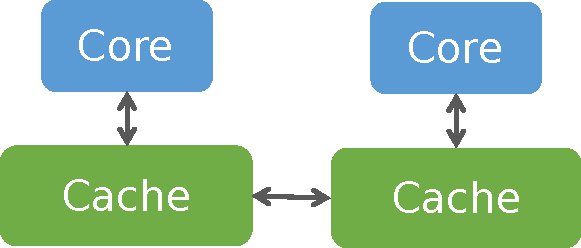
\includegraphics[width=1\columnwidth]{figs/cpumemmodel.pdf}
  \caption{Processor Architecture}
  \end{subfigure}
  \hfill
  \begin{subfigure}[b]{0.45\textwidth}
  \centering
  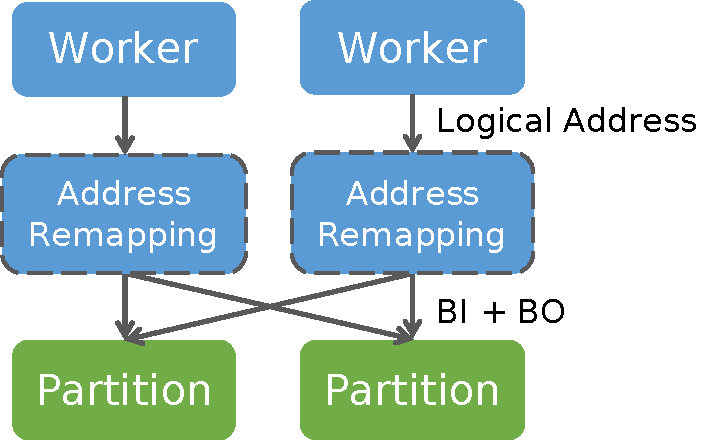
\includegraphics[width=1\columnwidth]{figs/spatialmemmodel.pdf}
  \caption{Reconfigurable Spatial Architecture}
  \end{subfigure}
  \caption[Memory model of different architectures]{Memory model of different architectures}
  \label{fig:memmodel}
\end{figure}
\begin{figure}
  \centering
  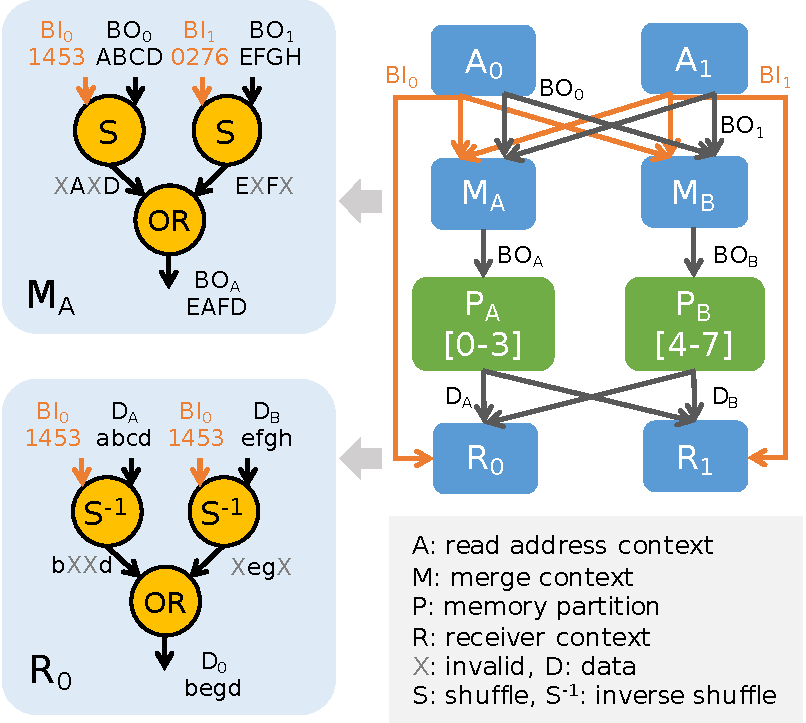
\includegraphics[width=0.6\columnwidth]{figs/memsplit2.pdf}
  \caption[Memory partitioning]{Example of memory partitioning across physical units. In this example, the program parallelizes the outer loop by two and vectorizes the inner loop by 4, which generates two vectorized access lanes. We need eight scratchpad banks to sustain the read bandwidth. 
  \name groups the 8 banks in two virtual memory partitions, $P_A$ (bank 0-3) and $P_B$ (bank 4-7). The address generation contexts $A_0$ and $A_1$ contains the computation for logical address and address remapping, which output $BA$s and $BO$s. \name allocates one merge context per memory partition
  ($M_A$ and $M_B$),
  merging requests from all access lanes. Inside the merge context, the shuffle operator converts the BO from access-aligned to bank-aligned. $A_0$, for example, requests offsets 
  A, B, C, and D ($BO_0$) from banks 1,4,5,and 3 ($BA_0$). The shuffle operator picks the requests belonging to partition A and outputs a BO aligned with bank 0-3. If the bank $i$ in the partition has no request, the $i$th element in the output is marked as invalid.
  The merge context contains one shuffle operator per request lane, and uses a tree of $OR$
  operators to combine all bank-aligned BOs into the final $BO_A$.
  On the receiver side, the memory broadcasts its response to all receiver lanes.
  The receiver context uses an inverse shuffle operator to convert the response from bank-aligned back to access-aligned, using the $BA$ forwarded from the address context. The response is then merged with another OR tree. 
  }
  \label{fig:memsplit}
\end{figure}

The coherence protocol is both expensive in hardware complexity and hard to scale in bandwidth for
streaming pipelined execution.
Instead of making redundant copies of the data, we can partition the data across different memory
partitions to get additional address port on a reconfigurable accelerator, as shown in
\Cref{fig:memmodel} (b).
Each parallel worker broadcasts the requests to all memory partitions.
If the data accessed by two parallel workers live in the same bank, the bandwidth will be halved.
To avoid bank conflicts, an important static analysis often used on reconfigurable accelerators is called static partitioning, or static banking~\cite{poly_cong}.
For most address patterns, the compiler can derive a partitioning scheme such that every partition is accessed by a
single worker at any time, which guarantees bandwidth at runtime.
The output of the analysis is an expression for bank address (BA) and bank offset (BO), both are
functions of the requested logical address.
BA determines which partition each request is going to, and BO is the offset within the
partition.

\Cref{fig:memsplit} shows how static banking is achieved on the Plasticine architecture.
Banking analysis from Spatial specifies the number of banks required to sustain bandwidth for the
current parallelization factors, and expressions for BAs and BOs. 
\name groups the banks into virtual memories, with group size limited by the number of banks in a PMU.
For each access lane, \name allocates a context to compute the logical and remapped address, which
outputs a vectorized BA and BO for each access lane. BAs and BOs are broadcasted to all memory partitions.
For each memory partition, \name allocates a merge context, merging BOs from all requesting lanes.
The merge context uses a shuffle operator to transform the vectorized BO from bank order specified by BA
(access-aligned) to bank order assigned to the current partition (bank-aligned).
Because the static banking analysis guarantees no bank conflicts for all banks,
\name can use a OR tree to merge the bank-aligned BOs into the final BO that gets send to
banks in the partition. On the receiver side, \name uses an inverse shuffle to convert responses from
partitions from bank-aligned back to access-aligned.
\name uses another OR tree to merge the access-aligned responses, which produces the final data
vector requested by the access lane.
With large parallelization, both the request OR tree and the respond OR tree can be
partitioned across VUs if running out of stages in a VU, scaling in the network bandwidth of the
crossbar connection by burning more VUs.

\Cref{sec:banking_arch} discusses the architectural changes to Plasticine to support this general
banking scheme.

\subsection{Register Allocation} \label{sec:regalloc}

After a VU is assigned to a PU, \name setups the configuration within a PU.
One of the configuration is assigning live variables in the dataflow graph to pipeline registers
across stages, shown in \Cref{fig:contexta}.

%\subsubsection{Blackbox IP Pruning} \label{sec:bbsplit}
%\yz{Cut this if out of the space}
%This step illustrates an example of integrating a customized partitioner for composable IP available on
%the architecture.
%The cost metrics and partition rule are specific to each IP.
%The example IP is a merge buffer, which can merge two sorted vector streams into a single stream with
%one vector per cycle throughput.
%The merge buffer pruner uses a tree of 2-way merge buffers across PUs to compose a multi-way merge buffer declared in the program.

\section{Optimizations}\label{sec:opt}
\name performs many of the standard compiler optimizations,
such as Dead Code Elimination and Constant Propagation.
Some of them, however, plays a much more important rule for reconfigurable accelerator because they
have direct impact on the resource usage.
Other optimizations can be counter-intuitive, as they introduce redundant computation that
reduces resource without necessarily impacting performance.
In this discussion, we focus our primary objective on performance.
Resource is an indirect objective as resource reduction enable larger parallelization factors,
, which in turn improves performance.

\subparagraph{Memory strength reduction (msr).} Like traditional strength reduction on arithmetics, \name{} replaces expensive on-chip memories with cheaper memories whenever possible.
%We map register accumulation in the program with single-cycle initiation interval to pipeline registers.
For example, \name{} replaces a scratchpad with constant address in all accesses to a un-indexable memory, such as a FIFO.
This commonly happens when producer and consumer loops of the memory are fully unrolled.

\subparagraph{Route-Through Elimination (rtelm).} For patterns where the content of a non-indexable memory  (M1) is read and written to another memory (M2), \name{} eliminates the intermediate access if the read of M1 and the write of M2 operates in lock-step.

\begin{figure*}
\centering
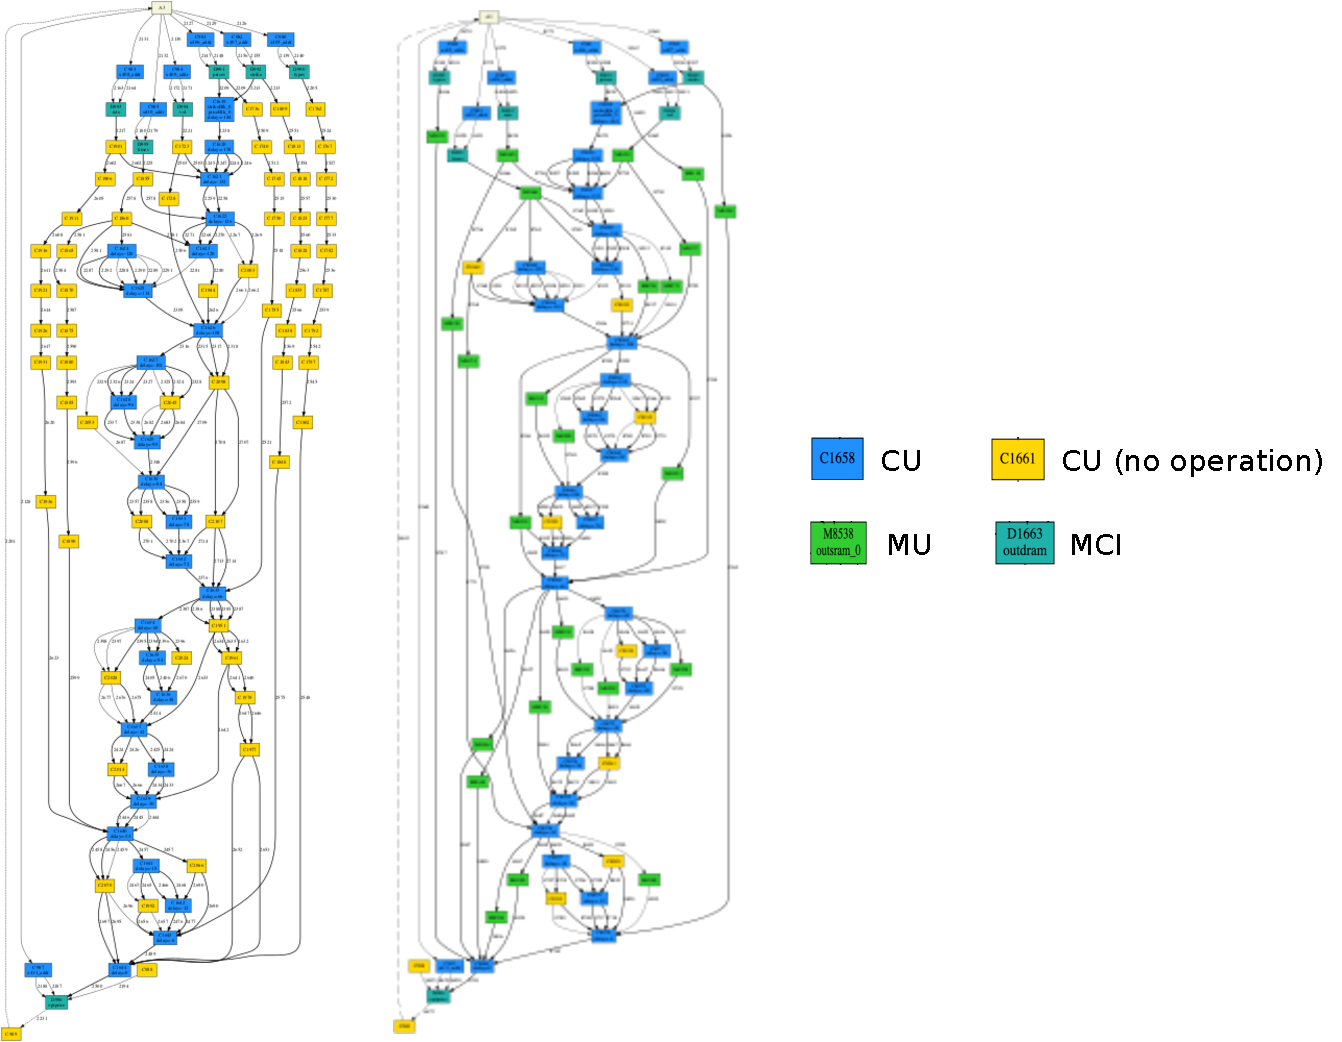
\includegraphics[width=0.7\textwidth]{figs/retiming.pdf}
\caption[Retiming]{
  Left: retiming with input buffer only. Right: retiming with either input buffer or scratchpad.
}
\label{fig:mlp}
\end{figure*}
\subparagraph{Retiming with scratchpad (retime-mem).} By default, \name{} uses PB input buffers for retiming purpose. 
This option enables \name{} to use scratchpad memory for retiming that requires large buffer depth.

\subparagraph{Crossbar datapath elimination (xbar-elm).}
Although, crossbars between accessors and memory partitions (\Cref{sec:memsplit}) are very expensive in the general case, the BI sometimes can be statically resolvable with certain combinations of parallelization on memory accesses. 
When BI is a constant, \name{} can use this information to intelligently assign virtual banks to partitions that reduce the crossbar data path to a partial or a point-to-point connection.

\subparagraph{Read request duplication (dupra).} During memory partitioning (\Cref{sec:memsplit}), instead of forwarding BI from the requester to receiver, \name{} can also duplicate the BI with local state on receiver side, which
eliminates the unbalanced data path at the cost of extra computation.

\begin{figure*}
\centering
\begin{subfigure}[b]{0.6\textwidth}
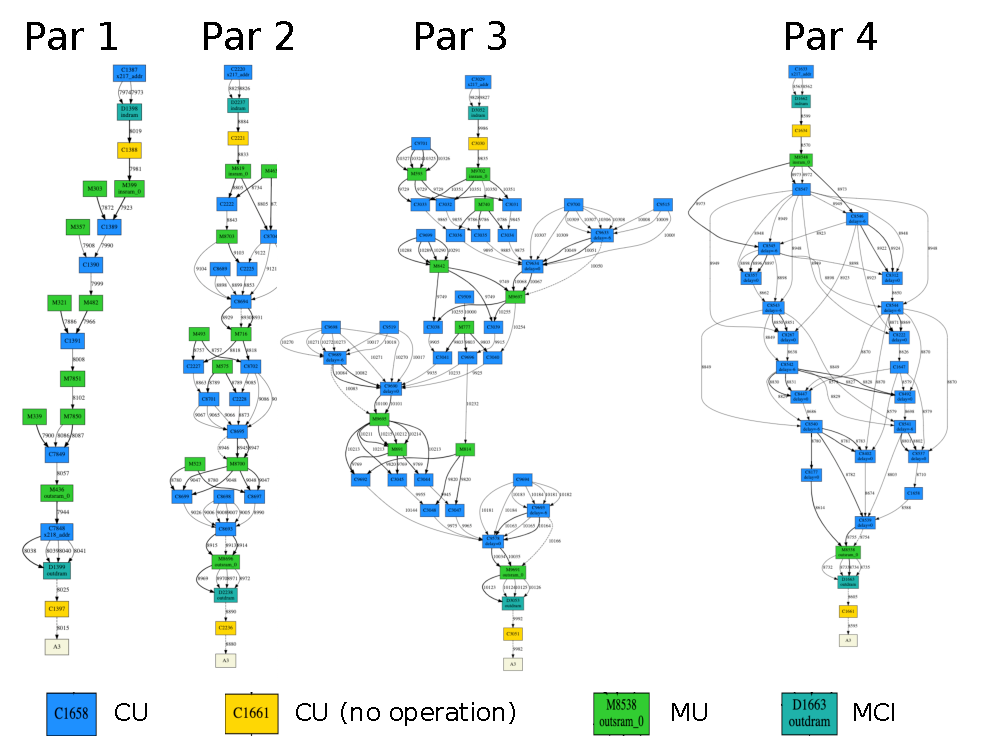
\includegraphics[width=1\textwidth]{figs/mlpunroll.pdf}
\caption{VUDFGs with different parallelization factors}
\end{subfigure}
\hfill
\begin{subfigure}[b]{0.39\textwidth}
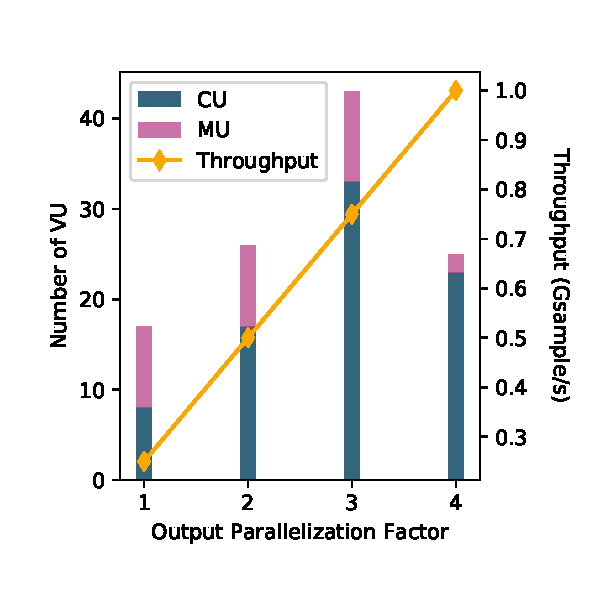
\includegraphics[width=1\textwidth]{figs/mlp.pdf}
\caption{Throughput and resource as a function of parallelization factor}
\end{subfigure}
\caption[MLP case study]{
  MLP case study
}
\label{fig:mlp}
\end{figure*}

\subparagraph{Global Merging (merge).}
After all VBs satisfy the hardware constraint, we perform a global optimization to compact small VBs into  larger VBs. 
Merging has very similar problem statement as compute partitioning (\Cref{sec:compsplit}) except with more constraints.
The traversal-based algorithm requires a reference cost for PB to check if the merged VB still satisfy the hardware constraint.
At each step of merging, we take the union of the domains of VBs within the current partition, and intersect with the domain of the merging VB.
The caveat is that even with a non-empty intersection, the bipartite graph might not have a possible assignment, as merged VB might fit in a larger PB with insufficient quantity.
Therefore, we perform a heuristic checking on feasibility of the bipartite assignment at each step of merging.
The solver-based solution combines partition assignment with PB type assignment as a joint problem. 
The output of merging gives both partition assignment as well as a PB type assignment, which eliminates the risk of un-mappable bipartite graph due to merging in the traversal-based solution.

\subparagraph{Memory Localization}
We perform another specialization on non-indexable memories (registers or FIFOs), whose all accesses have no explicit read enables.
Instead of treating them as shared memories, \name{} duplicates and maps them to local input buffers in all receivers, no longer requiring tokens.
The sender actor pushes to the network when the token is supposed to be sent, and the receiver dequeues one element from the input buffer when the token is supposed to be consumed.
This dramatically reduces the synchronization complexity of non-indexable memory in the common case.

\subparagraph{Reverse Loop Invariant Hoisting}
A common loop optimizations is to move loop invariant expressions outside of the loop body to reduce
computation. This optimizations, however, might introduce more basic blocks in the program.
For Plasticine, number of basic blocks have a strong correlation with number of contexts and
physical units. \Cref{fig:reversehoisting} shows an example where moving instructions into the loop
body reduces number compute units. Because instructions within basic blocks and basic blocks
themselves are pipelined, doing so does not have performance impact on the application.
Currently, we rely on the user to perform manually perform this optimization.

\begin{figure*}
\centering
\hfill
\begin{subfigure}[b]{0.4\textwidth}
\inputminted{python}{code/hoisting.py}
\caption{Input program}
\end{subfigure}
\hfill
\begin{subfigure}[b]{0.4\textwidth}
\inputminted{python}{code/reversehoisting.py}
\caption{Reverse Loop Invariant Hoisting}
\end{subfigure}
\hfill
\caption[Reverse Loop Invariant Hoisting]{
  The original program requires at least two contexts to execute Block 1 and Block 2.
  By moving the invariant instruction \texttt{c = a + b} into the loop body, (b) only needs a single
  context instead. Because instructions within \texttt{Block 2} are pipelined across loop
  iterations, adding instructions in the loop body introduce minimum performance impact.
  This transformation is beneficial until \texttt{Block 2} exceeds six operations, at which point
  both version consume the same amount of resources.
}
\label{fig:reversehoisting}
\end{figure*}

\begin{figure*}
\centering
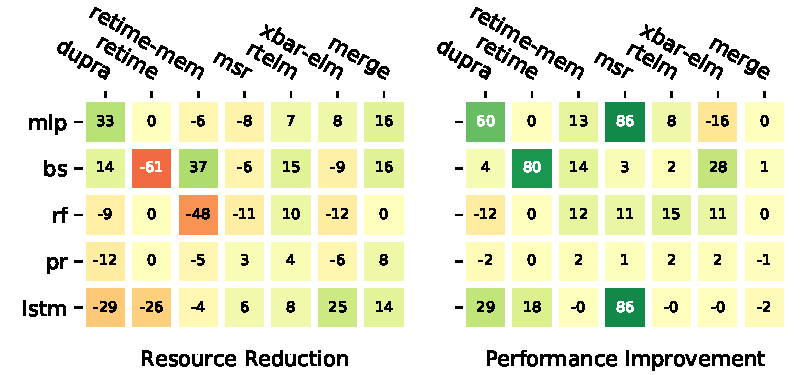
\includegraphics[width=0.7\textwidth]{figs/heat.pdf}
\caption[Optimization Effectiveness]{
  Optimization Effectiveness. Percentage resource reduction or performance improvement from each
  optimization. The heat map shows the maximum differences when turning on/off the optimization, 
  while keeping other optimizations the same.
  For a single application, the improvement is taking the geometric mean across different application parameters.
}
\label{fig:reversehoisting}
\end{figure*}

\begin{figure*}
\centering
\hfill
\begin{subfigure}[b]{0.35\textwidth}
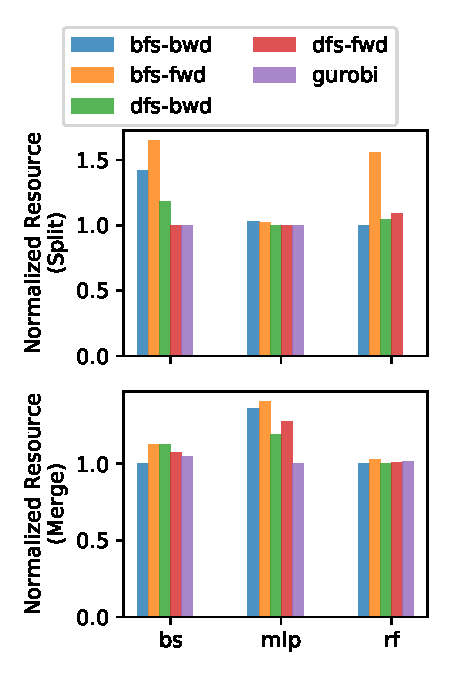
\includegraphics[width=1\textwidth]{figs/algo2.pdf}
\caption{Resource Comparison}
\end{subfigure}
\hfill
\begin{subfigure}[b]{0.64\textwidth}
\centering
\begin{tabular}{lccccc}
  \toprule
  Apps &bfs-bwd & bfs-fwd & dfs-bwd & dfs-fwd & gurobi \\ \midrule 
bs & 3s & 3s & 2s & 2s & 2h4m \\ 
mlp & <1s & <1s & <1s & <1s & 4s \\ 
rf & 1m37s & 1m7s & 29s & 27s & - \\ 

 \bottomrule
\end{tabular}
\caption{
  Compile time for spltting
}
\vspace{0.1cm}
\begin{tabular}{lccccc}
  \toprule
  Apps &bfs-bwd & bfs-fwd & dfs-bwd & dfs-fwd & gurobi \\ \midrule 
bs & 1s & 2s & 5s & 3s & 1m4s \\ 
mlp & 5s & 5s & 6s & 11s & 31m16s \\ 
rf & 11s & 10s & 2m7s & 1m0s & 14h27m \\ 

 \bottomrule
\end{tabular}
\caption{
  Compile time for merging
}
\vspace{0.65cm}
\end{subfigure}
\hfill
\caption[Partitioning and merging algorithm comparison]{
  Partitioning and merging algorithm comparison. (a) shows the normalized resource usage between
  different algorithms (the lower the better). (b) and (c) shows the compile time of each algorithm.
}
\label{fig:split}
\end{figure*}
%\subparagraph{Dead Code Elimination (DCE)} 
%We perform aggressive DCE on the VBDFG and only keeps computation that gets materialized to accelerator I/O and DRAM.
%\subparagraph{Constant Propagation}
%Aside from regular constant propagation on arithmetics, we also eliminates crossbar datapath when bank ID 
%can be statically resolved described later in \Cref{sec:memsplit}.
%During loop unrolling, address of indexable memory sometimes can be resolved to static constant.
%For a read-only RAM with constant address, we lookup their content at compile time and embed its content into registers.
%For \emph{route-through} pattern, where content of a non-indexable memory M1 is read and written to another memory M2,
%we can eliminate the intermediate write and forward the data directly to the final memory if the compiler
%can prove the read M1 and write of M2 operates in lock-step.
%We also perform constant propagation on control signals with loop-range analysis. 
%Eliminates the control signals can expose more lock-step accesses and \emph{route-through} opportunities.
%\subparagraph{Strength Reduction}
%In addition to traditional strength reduction on arithmetics, we also replace expensive memories
%with cheaper memory whenever possible.
%We map register accumulation in the program with single-cycle initiation interval to pipeline registers.
%Banked-SRAM with constant bank IDs and offsets in all accessors can also be replaced with FIFOs,
%which is happens when producer and consumer loops are fully unrolled.

%Accesses statically banked in the input graph can operates concurrently 
%without bank conflicts, as explained in \Cref{sec:background}.
%These accesses are usually from a unrolled loops. For banked accesses from the same pre-unrolled access, 
%\name first merge all requests before sending to the memory (details in \Cref{sec:memsplit}). 
%Because these accesses are from loop unrolling, they have the same program order and same dependency with other accesses.
%So the synchronization can be performed on the merged access, which prevents the amount of synchronization
%to increase with parallelism on a banked memory, as shown in \Cref{fig:mergetoken}

%\subsubsection{Blackbox IP Pruning} \label{sec:bbsplit}
%\yz{Cut this if out of the space}
%This step illustrates an example of integrating a customized partitioner for composable IP available on
%the architecture.
%The cost metrics and partition rule is specific to each IP.
%The example IP is a merge buffer, which can merge two sorted vector streams into a single stream with
%one vector per cycle throughput.
%The merge buffer pruner uses a tree of 2-way merge buffers across PBs to compose a multi-way merge buffer declared in the program.



\section{Placement and Routing} \label{sec:par}
The input to the \emph{placement and routing (PaR)} phase is a VUDFG, with each VU tagged to a PU
type.
Before PaR, \name also performs a runtime analysis of the program, annotating each edge in the VUDFG
with a link priority. The link priority is used to determine the routing order during PaR.
PaR then iteratively places VUs and route edges in VUDFG onto the global network.

In addition to the original static network in Plasticine, we introduce a dynamic network in
parallel to the static network, forming a dynamic-static hybrid network.
Both purely static and purely dynamic networks are instances of the parameterized hybrid network.
\Cref{sec:network} will discuss the details about the hybrid network.
The PaR algorithm needs to handle both network types and multiple network granularity (vector,
scalar, control) at the same time.

The major difference between the static and the dynamic network is that each physical link in the static network is dedicated to a logical edge in the VUDFG for the entire duration of the execution
(circuit-switching\footnote{Technically, our static network is more restrictive than
circuit-switching because circuit-switching allows deallocation after the connection is terminated.
Our static network, on the other hand, cannot be reconfigured until the application terminates.}), whereas 
the physical link in the dynamic network can be time-shared by multiple logical edges
(packet-switching).
Both static and dynamic networks are statically routed by the PaR algorithm. 
For a dynamic network, PaR also needs to assign virtual channels (VCs) to prevent network deadlock.
The PaR algorithm configures the lookup table in each router that maps the packet header to the
destination port and VC.

In the rest of this section, \Cref{sec:place} and \Cref{sec:route} discusses the placement 
and the routing algorithm. 
\Cref{sec:vc} explains the need for VC allocation. 
Lastly, \Cref{sec:heuristic} describes how \name generates link priority.

\subsection{Iterative Placement} \label{sec:place}

At high-level, the PaR algorithm works very similarly to the FPGA PaR using
simulated annealing~\cite{simanneal}. 
For the initial placement, the algorithm places VUs in VUDFG in topological order.
Each VU is placed to the next available PU with minimum Manhattan distance to the placed
neighbors of that VU.
Next, the algorithm routes all edges in the VUDFG, starting from edges with the highest link
priority. If no routes are available on the static network, the route will be moved onto the dynamic
network. For purely static networks, there is an ``imaginary'' dynamic network for this step.
If there are still routes on the fake dynamic network at the end of the PaR, PaR is considered
failed for the purely static network.
After all routes are routed, either on the static or dynamic network, the PaR evaluates the
congestion cost of the current placement.
Then, a genetic algorithm shuffles the VUs whose edges contribute most to congestion, 
and keeps the new position if it improves the route assignment.
By iteratively re-placing and re-routing, the mapping process eventually converges to a good placement.

The PaR uses a heuristic cost model to rapidly evaluate placements: a 
penalty score is assigned as a linear function of several subscores.
These include projected congestion on dynamic links, projected congestion at network injection and ejection ports, the average route length, and the length of the longest route.
\name provides a static estimate of the number of packets sent on each logical link.
The PaR algorithm estimates congestion by normalizing the number of packets on each link to the program link with the highest total packet count.
The most active program link sets a lower bound on the program runtime (the highest bandwidth physical link can still only send one packet per cycle), which translates to an upper bound on congestion for other links.

%The {\sc Unplace} function randomly decides between unplacing a random node, and unplacing one or several nodes based on heuristics.
%For the heuristic-based unplacement, a node's contribution to global route congestion is calculated by adding an estimate of all connected routes' contributions to the global penalty score; the node(s) with the highest scores are unplaced.
%Similarly, {\sc Place} also can either randomly place an unplaced node, or place it to minimize the Manhattan distance to its logical neighbors. {\sc Score} calculates the heuristics for each node, and {\sc Filter} duplicates the best candidate placements to fill the pool. Because the unplacement and replacement steps can make a placement worse, the best performing placements are frozen in each iteration to ensure that no good placements are thrown away.

\subsection{Congestion-Aware Routing} \label{sec:route}
%\info{Somewhere we should mention that placement and routing running interchangeably}
To achieve optimal performance, we use a routing algorithm that projects congestion and routes around it. 
Routing starts with the highest-priority routes, as determined by fanout of the broadcast edge and
estimated packet count; broadcast edge with higher fanout is harder to route and hence are routed
first.
Using the packet count as a priority makes sure that the static network is used most efficiently.
Our scheme searches a large space of routes for each link, using Dijkstra's algorithm \cite{dijkstra} and a hop weighting function.
To ensure maximum link reuse in broadcast edges, we can augment the hop weight in Dijkstra's
algorithm by a multiplication factor between zero and one. 
When finding the shortest path between each source-destination pair, the weight of the hop is
multiplied by the factor each time the hop is reused for the same broadcast edge.
In other words, the reused path has a lower hop cost compared to other paths.
This trick provides a balance between the shortest path and link reuse: a smaller factor encourages link
reuse, even though individual source-destination pairs are not the shortest path; a factor equals to 1 ensure all source-destination pairs are routed with the shortest path.
The second objective for routing broadcast links is balancing the hop counts between all
destinations. This is because the shorter path will back pressure the sender before packets reaching to the longer path, causing pipeline stalls.
To achieve this, we start with the source-destination pair with the longest Manhattan distance, ensuring
the most far apart source-destination pair is routed on the shortest path.
The consecutive source-destination pairs will try sharing the link on this path and slightly detour from
their shortest path, which balances the hop count.
%Routes are not analyzed on the basis of a single source-destination pair, which would be inadequate for broadcasts: instead, a directed graph is built from the source and all destinations in the route, with edge weights corresponding to the minimal route between each pair of VUs in the broadcast.
%For example, if the broadcast is from VU-1 to VU-2 and VU-3, four total potential routes are analyzed for congestion: VU-1 to VU-2, VU-1 to VU-3, VU-2 to VU-3, and VU-3 to VU-2.
%The routes are weighted so that routes mapped on the static network are preferable to those mapped to the dynamic network; within these categories, routes are weighted based on length. 

%\info{does the nodes refer to only source and destinations or including all nodes on the path between source and destination. How does the weights represent the minimum routes? Is it capturing the cost of the minimum route?}
%Then, a search algorithm based on Prim's algorithm for minimum spanning trees \cite{prim1957shortest} is run to build a tree for the broadcast, starting with only the source being reached.
%At every step, the most-preferable route (from the graph built using Dijkstra's algorithm) that adds a new destination VU to the reached set is chosen and added to the broadcast, until all destination VUs are reached. 
%This route can start from either the source of the broadcast tree or any destination currently in the reached set.
%The algorithm will find a fully static broadcast tree, if one exists, and will only add a non-static route to the broadcast (moving the entire broadcast to the dynamic network) when there are VUs in the tree that cannot be reached from the source VU by \emph{any} static route.
%\info{does the algorithm routes links from high priority to low from all nodes or it does one node at a time?}

\subsection{VC Allocation for Deadlock Avoidance} \label{sec:vc}
Deadlock is a system pathology in dynamic routing where multiple flits form a cyclic holds on/waits for dependency on each others' buffers and prevent forward progress.
Most dataflow accelerators use a streaming model, where outputs of a producer are sent over the network to one or more consumers
without an explicit request; the producer is backpressure when there is insufficient buffer space. 
While this paradigm improves accelerator throughout by avoiding the round-trip delay of a request-response protocol, it introduces an additional source of deadlock \cite{hansson2007avoiding}. 

\Cref{fig:deadlock}(a) shows a sample VUDFG graph, which is statically placed and routed on a $2\times3$ network in (b). 
Logical edges B and C share a physical link in the network. If C fills the buffer shared with B, VU-3 will never receive any packets from B and will not make forward progress.
%For y-z dimension-order routing, the only valid routes from VU-1 to VU-3 is through $\[0,1\], \[0,0\], \[1,0\], \[2,0\]$. 
%Dimension-order routing prevents deadlock by eliminating cycles in network routes.
%On traditional NoCs, deadlock can be solved with dimension-order routing, which routes all traffic on one dimension before another.
%\yaqi{
  With streaming computation, the program graph must be considered as part of the network dependency graph, which must be cycle-free to guarantee deadlock freedom. However, this is infeasible because cycles can exist in a valid VU dataflow graph when the original program has a loop-carried dependency. Therefore, deadlock avoidance using cycle-free routing, such as dimension-order routing, does not work in our scenario. 
Allocating VCs to prevent multiple logical links from sharing the same physical buffer is consequently the most practical option for deadlock avoidance on streaming accelerators.
%Because the entire program is connected through these streaming dependencies, any two links can conflict and result in a deadlock.
%\yaqi{However, cycles are permitted in the programming paradigms since loop-carried dependencies can be mapped across the network.
%Therefore, we perform VC allocation at each router to prevent multiple logical links from sharing the same physical buffer.
\if 0
Virtual channel (VC) allocation is another common approach to avoid deadlock. We can statically assign conflicting streams B and C with different
virtual channels at router $[2,0]$, which prevents them to share physical buffers. 
Notice indirect inputs of a VU, such as A and D with eventual consumer VU-3,
also need distinct VCs to ensure deadlock-free. To minimize the number of VCs required, we perform per-hop VC allocation--statically
assign conflicting links at each input of each router with distinct VCs. The VCs can be looked up at runtime based on link ID.
Distinct links from the same source VU, such as A and C, can share the same VC because VU-1 ensures the number of flits sent over A and C remains
to a ratio that the receiver expects, which permits data to drain in the network.
\fi

\begin{figure}
\centering
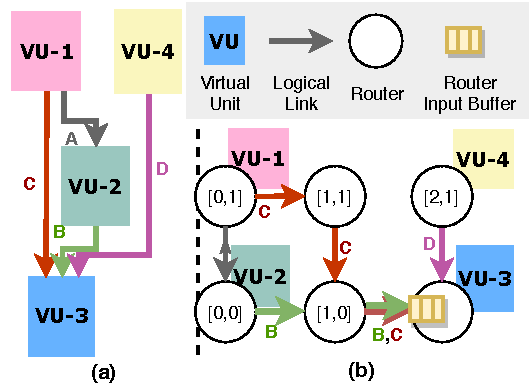
\includegraphics[width=0.4\columnwidth]{figs/deadlock.pdf}
  \caption[Network deadlock in streaming accelerators]{An example of deadlock in a streaming accelerator, showing the (a) VU data-flow graph and (b) physical placement and routes on a $2\times3$ network. There are input buffers at all router inputs, but only the buffer of interest is shown.}\small\textsuperscript{}\label{fig:deadlock}
\end{figure}

\subsection{Runtime Analysis for Heuristic Generation} \label{sec:heuristic}

In Spatial, users can annotate the value of runtime variables to assist compiler analysis.  
We use these programmer annotations to compute the expected number of iterations each basic block
will execute. 
The execution count on the basic block can further be used to derive the packet counts produced
by these basic blocks.
For a loop with data-dependent bounds, the user can annotate an estimate of the bound value.
For a branch statement, the user can annotate a percentage distribute between the if and else clauses.
The runtime of a streaming program is a function of the number of packets received on the incoming
stream. 
Static runtime analysis can identify potential application-level deadlock due to stream mismatching, as shown
in \Cref{fig:runtime}.

The derived packet counts based on these annotations can help the placer to evenly spread out the traffic.
The placer prioritizes highly used links on the static network and leaves infrequently used links on the dynamic network. 
However, we do not require exact annotations for efficient placement---rough estimates of these runtime values are sufficient to determine the relative importance of links.
When no annotation is provided, the compiler estimates
loop iteration counts based on the nesting depth: packets generated by the innermost loops are 
the more likely to be frequent.
This heuristic provides a reasonable estimate of links' priorities for routing purposes.

\begin{figure*}
\centering
\begin{subfigure}[b]{0.8\textwidth}
\inputminted{python}{code/runtime.py}
\caption{Example program}
\end{subfigure}
\caption[Runtime analysis]{
  Example of a streaming program whose runtime depends on the number of packets received on
  \texttt{stream}. We use a \texttt{queue} to model a stream receiving the packets from the
  network.
  Loop \emph{A} is a forever loop whose runtime is determined by its child controllers.
  With user annotation on number of packets from \texttt{stream}, 
  we know the runtime of loop \emph{B} is $T(B) = N$.
  As a result, we can derive the runtime of loop \emph{B}'s and parent \emph{A}, 
  i.e. $T(A) = \lceil\frac{N}{B}\rceil$. 
  With runtime for $A$, the runtime for $C$,$D$,and $E$ can be computed as
  $T(C) = \lceil\frac{N}{B}\rceil\cdot C$,
  $T(D) = \lceil\frac{N}{B}\rceil\cdot C \cdot R$, 
  and $T(E) = \lceil\frac{N}{B}\rceil\cdot C \cdot R \cdot E$.
  The runtime for \emph{E} also depends on \texttt{q}, which gives $T(E) = T(B) = N$. 
  If $\lceil\frac{N}{B}\rceil\cdot C \cdot R \cdot E \neq N$, \name gives an warnning for the
  inconsistency that potentially triggers an undesired deadlock.
}
\label{fig:runtime}
\end{figure*}

%\section{Debugging and Instrumentation Support (WIP)}
%\subsubsection{Deadlock in Streaming Reconfigurable Architecture}

%\subsubsection{Debugging Support and Performance Instrumentation}

\section{Evaluation (WIP)} \label{sec:eval}

\begin{figure*}
\centering
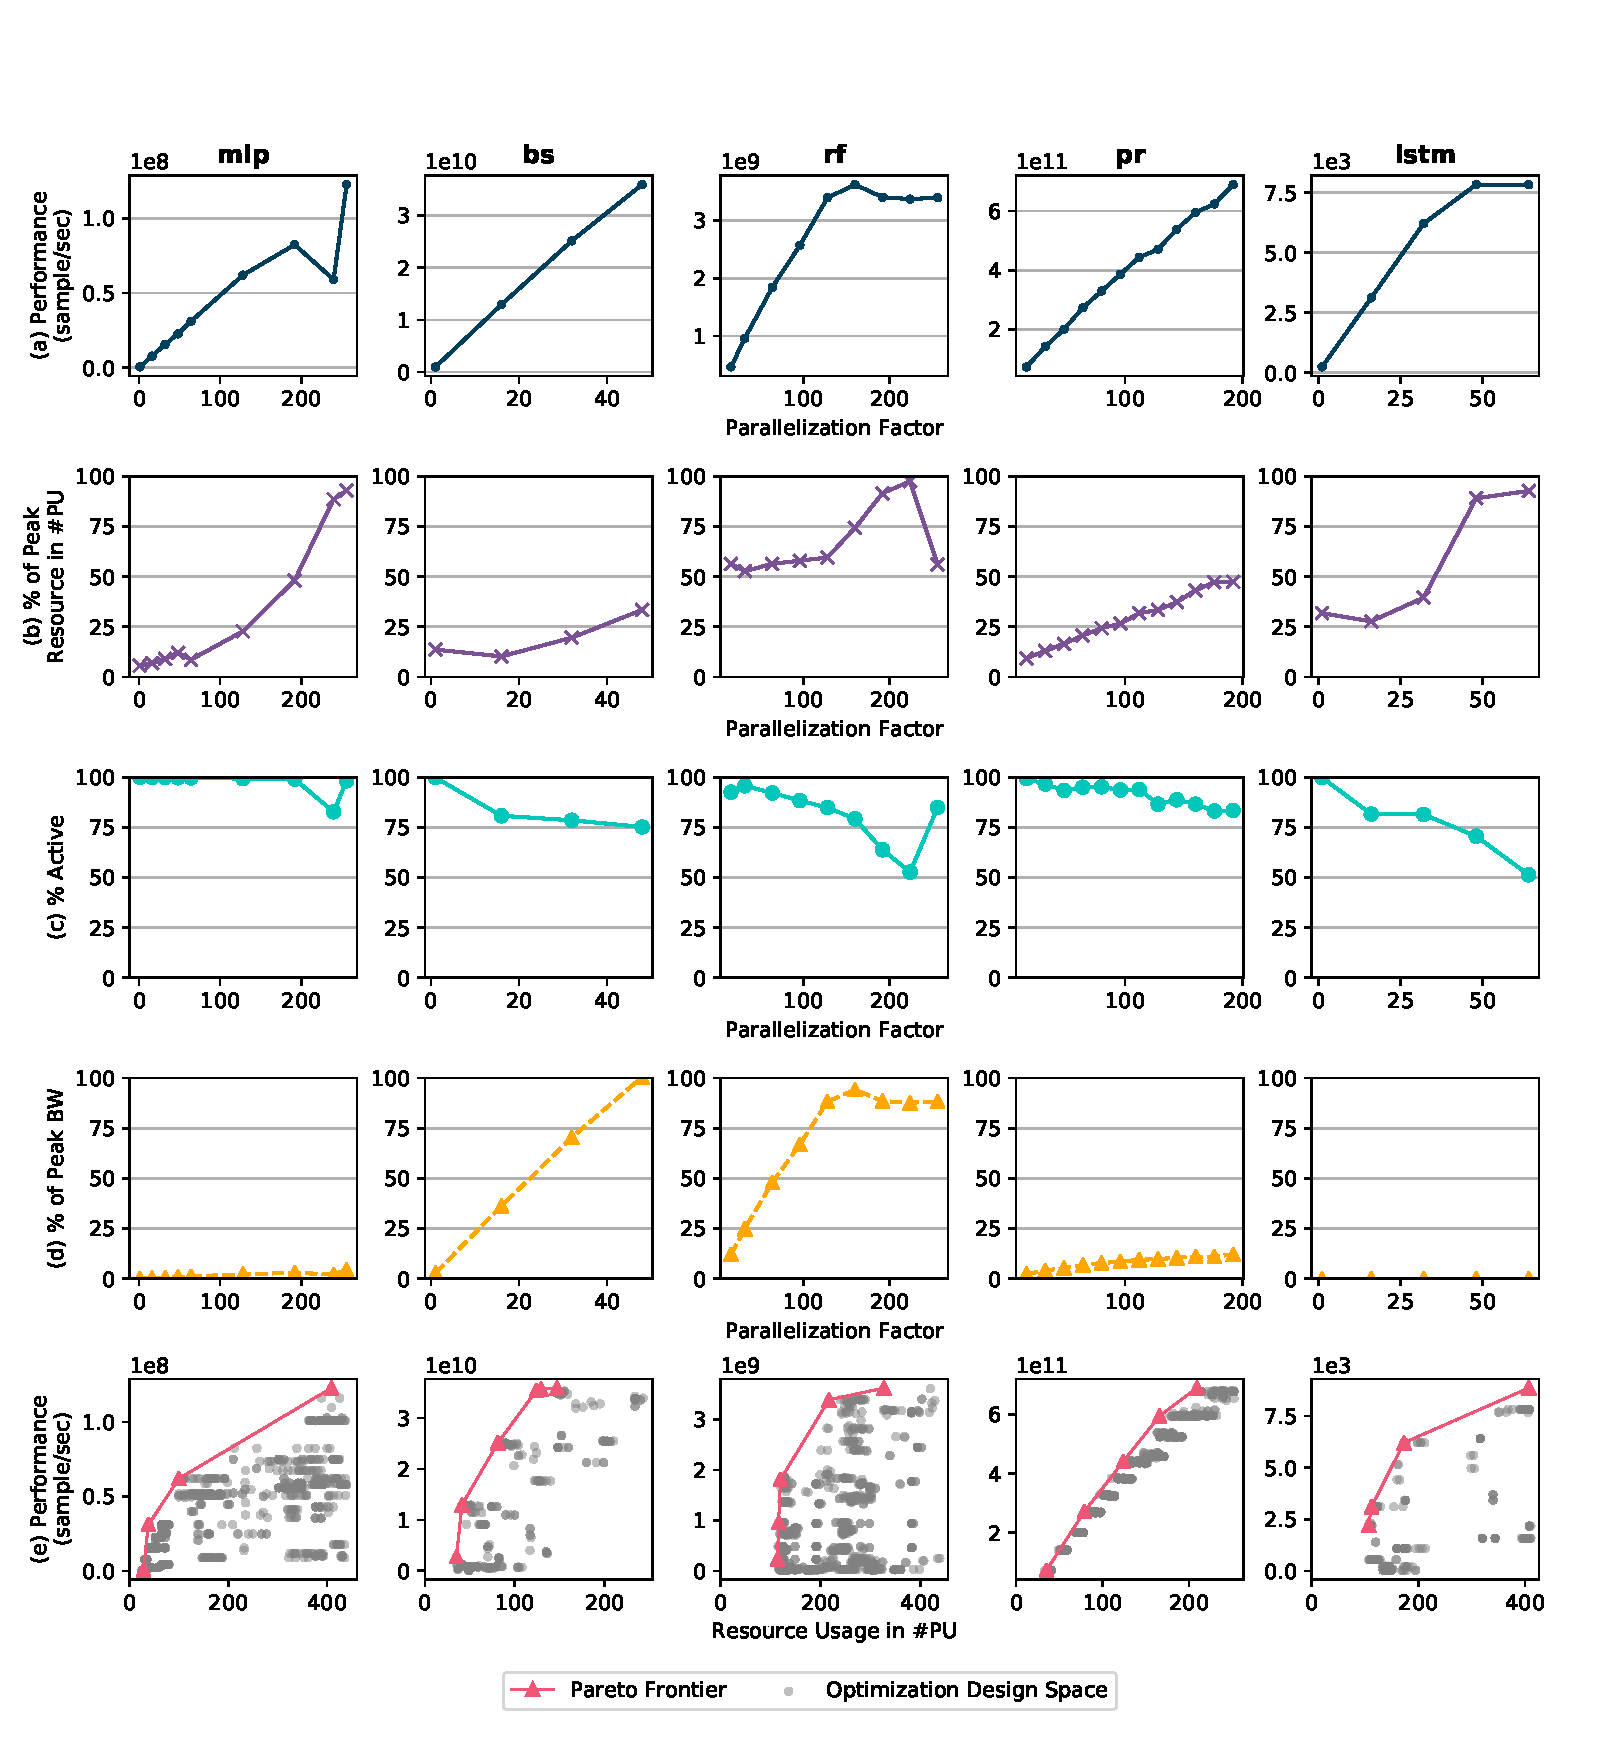
\includegraphics[width=1\textwidth]{/Users/yaqiz/pldi20/paper/figures/par_thesis.pdf}
\caption[Scalability Evaluation]{
  Scalability Evaluation. 
  The first four charts show the scaling of
  (a) throughput, 
  (b) resource usage, 
  (c) runtime activation rate of PUs on the critical path of the compute pipeline, 
  and (d) achieved HBM bandwidth, as the program gets parallelized.
  (e) shows the combined design space of compiler optimizations and parallelization factors on a
  throughput-resource curve. 
  The pareto frontier presents the throughput shown in (a) as a function of resource increase in
  (b).
}
\label{fig:par}
\end{figure*}

%\begin{figure*}
%\centering
%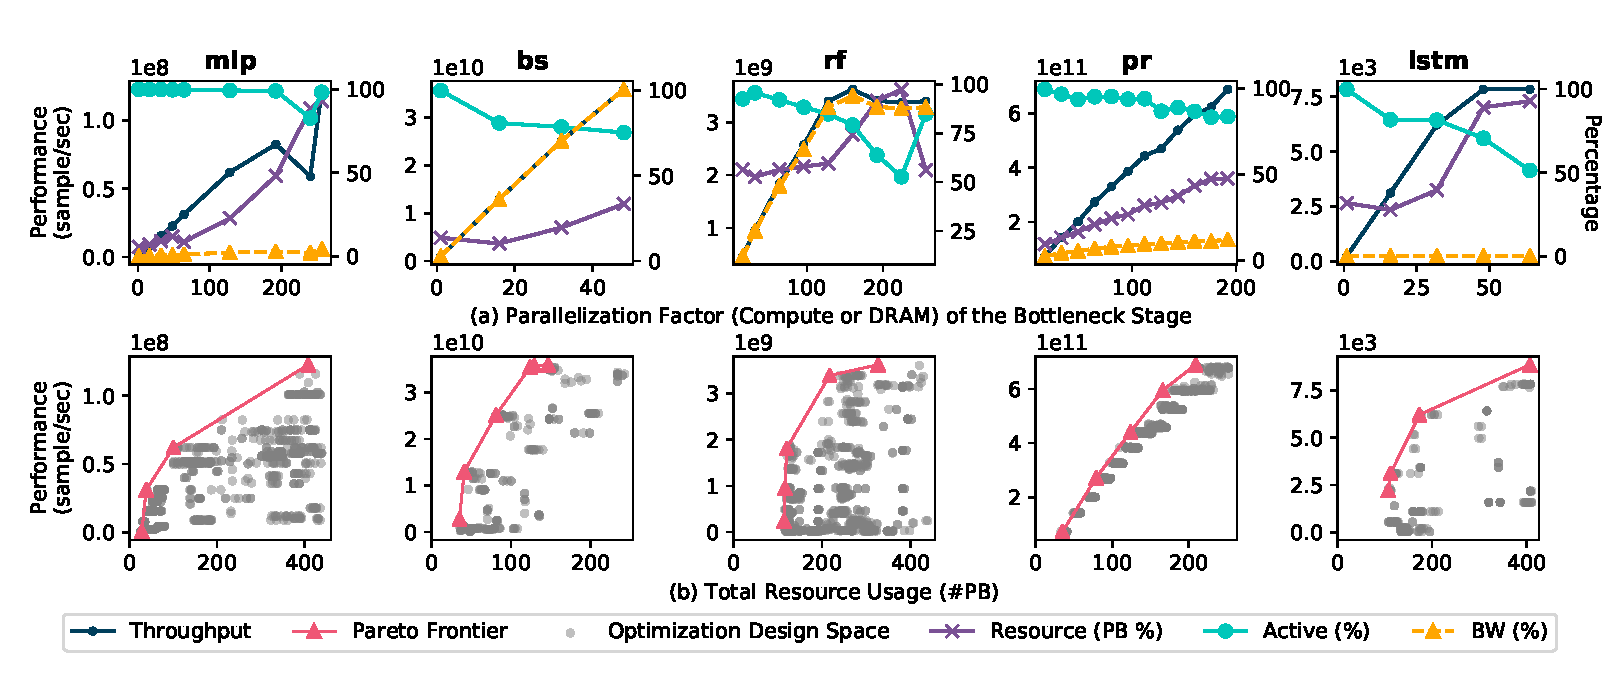
\includegraphics[width=1\textwidth]{/Users/yaqiz/pldi20/paper/figures/par.pdf}
%\caption[Performance comparison with V100 GPU]{
%}
%\label{fig:par}
%\end{figure*}

\begin{table}[t]
  \centering
    \footnotesize
    \begin{tabular}{lcccccc}
    \toprule
      \multirow{2}{*}{\textbf{Benchmark}} &
      \multirow{2}{*}{\makecell[c]{\bf Throughout\\\bf Unit}} &
      \multirow{2}{*}{\makecell[c]{\bf GPU\\\bf Compiler}} & \multicolumn{2}{c}{\textbf{Latency} (ms)} &
      \multicolumn{2}{c}{\textbf{Throughput} (Unit/s)} \\
                                & & & \name & GPU & \name & GPU     \\
      \midrule
        SqueezeNet (batch-1) & {\em kFrames}   & TF+cuDNN & 49.13  & 70.10  & 0.12 (1.1) & 0.4   \\ \addlinespace
        LSTM (batch-32)      & {\em kSamples}  & TF+cuDNN & 3.61   & 6.81   & 8.8 (79.2) & 4.7   \\ \addlinespace
        PageRank             & {\em MEdges}    & GunRock & 128.27 & 829.39 & 49         & 7.5   \\ \addlinespace
        BlackScholes         & {\em GOptions}  & CUDA & 0.09   & 0.10   & 88.88      & 80.02 \\ \addlinespace
        Random Forest        & {\em MSamples}  & CUDA & 0.10   & 0.32   & 1.04       & 0.32  \\ \addlinespace
        Merge Sort           & {\em GElements} & CUDA & 0.63   & 2.14   & 6.65       & 1.96  \\
      \bottomrule
    \end{tabular}
  \caption{Performance comparison of Plasticine with Tesla's V100 GPU (Normalized throughput to transistor count in parentheses).}
  \label{tab:gpu-comparison}
\end{table}
\begin{figure*}
\centering
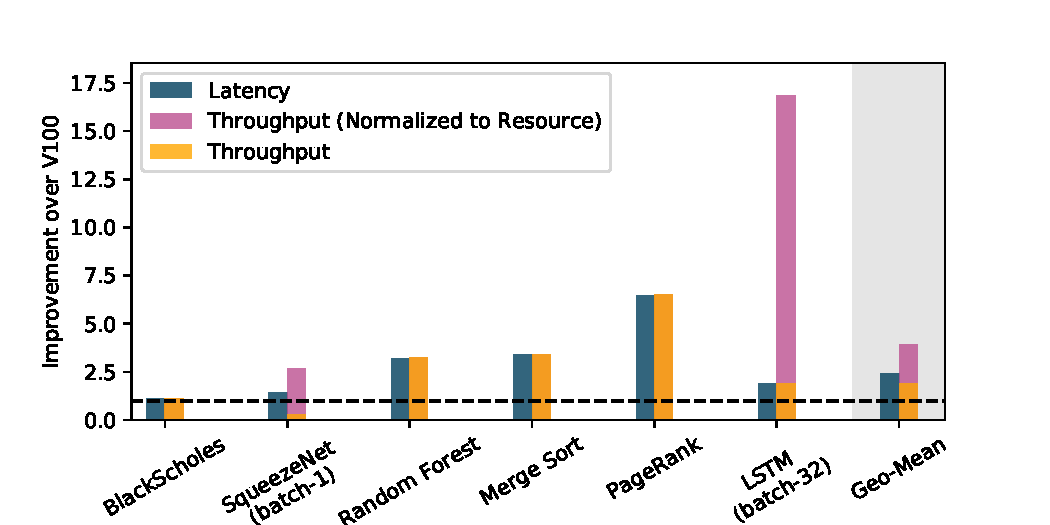
\includegraphics[width=1\textwidth]{figs/slide_gpu.pdf}
\caption[Performance comparison with V100 GPU]{
  Plasticine's latency and throughout improvement over V100 GPU.
  The evaluated Plasticine architecture has area footprint of 352$mm^2$ at 28nm.
  V100 GPU has area footprint of 815$mm^2$ at 12nm.
  Both platforms have the same off-chip bandwidth at 1TB/s with HBM technology.
  Yellow and blue bars show the raw measured speedup in throughput and latency, respectively.
  To account for the resource discrepancy, the pink bar shows the normalized throughput
  for compute-bound application--SqueezeNet and LSTM, which scales performance with additionally
  on-chip resources.
}
\label{fig:peakutil}
\end{figure*}


\section{Evaluation} \label{sec:eval}

%% Recap work flow for readers
To evaluate our compilation flow and network architectures, we use a set of benchmarks implemented in Spatial. 
%We connect the Spatial's output IR with our low-level compiler described in section~\ref{sec:compiler}.
We start with Spatial's output IR (Section~\ref{sec:compiler}), and transform it into a graph of distributed, streaming VBs.
Our compiler then performs place and route for a target architecture before generating a configuration for cycle-accurate simulation. 
During simulation, we track the amount of data moved by each switch and router, which we integrate with synthesis results to produce estimates of area and power.

For each application, we find the highest-performing parallelization and tiling factors; for DRAM-bound applications, this is the configuration that saturates memory bandwidth.
The optimum parameters for each network configuration may vary, as high parallelization does not improve performance on a low bandwidth network.
%Next, for each optimized application, we evaluate network configurations as described in Section~\ref{sec:net_dse}.
We start with benchmark characterizations (Section~\ref{sec:app_char}), analyzing application characteristics and communication patterns to identify how they interact with networks.
Next, we characterize the area and energy of network primitives, which we use to calculate the total network area and energy in Section~\ref{sec:net_char}. 
Finally, Section~\ref{sec:network} presents a design space study over all network dimensions for both pipelined and scheduled architectures. 
Table~\ref{tab:notation} summarizes the notation we use to describe network configurations in the remainder of this section.

\subsection{Application Characterization} \label{sec:app_char}

\begin{figure}
\centering
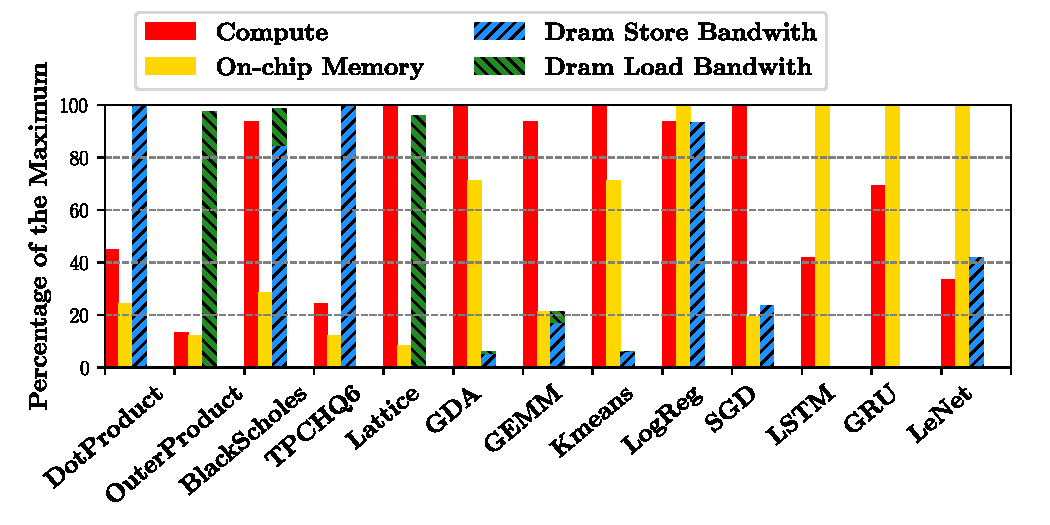
\includegraphics[width=1\columnwidth]{figs/util_bw2.pdf}
\caption{Physical resource and bandwidth utilization for various applications.}\label{fig:util_bw}
\centering
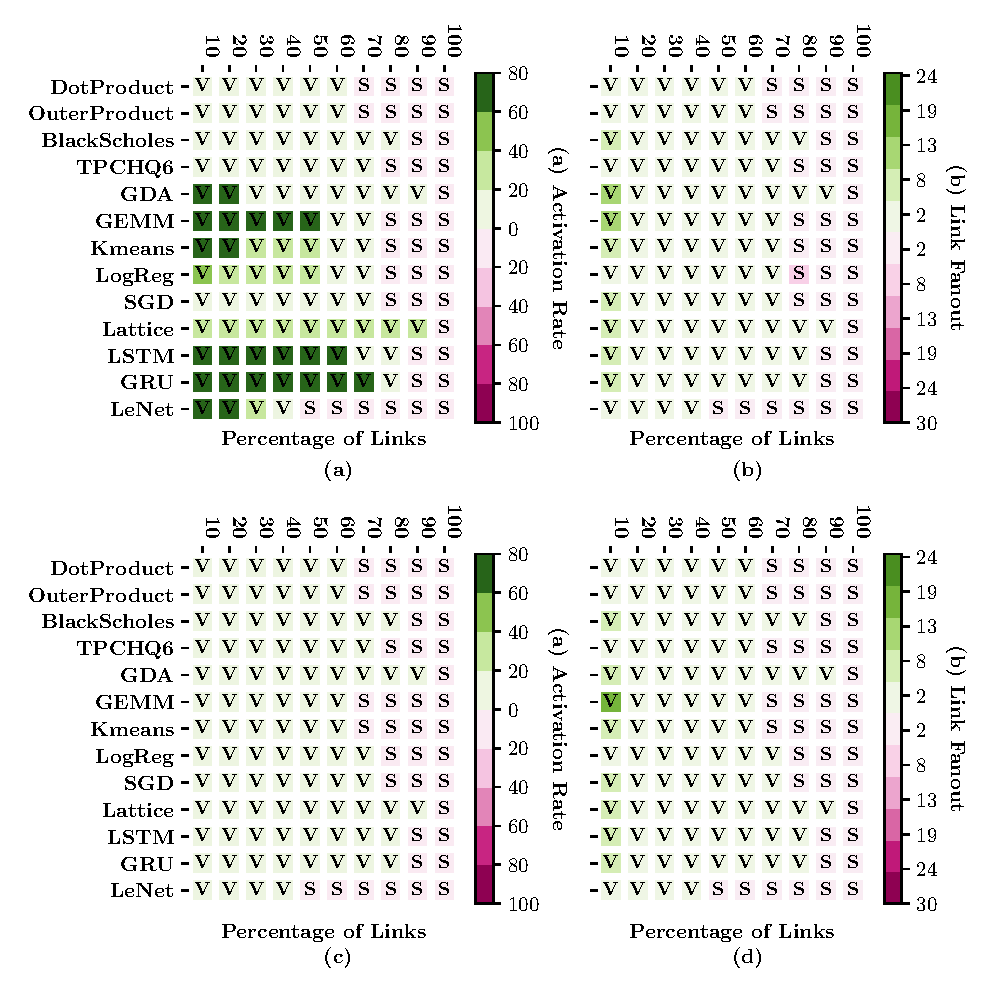
\includegraphics[width=1\columnwidth]{figs/link7.pdf}
  \caption{Application communication patterns on pipelined (a,b) and scheduled (c,d) CGRA architectures.
  (a) and (c) show the activation rate distribution of logical links at runtime. 
  Links sorted by granularity, then rate; darker boxes indicate higher rates.
  The split between green and pink shows the ratio of logical vector to scalar links. (b) and (d) show the distribution of broadcast link fanouts.
 }\label{fig:link}
\end{figure}

\begin{figure}
\centering
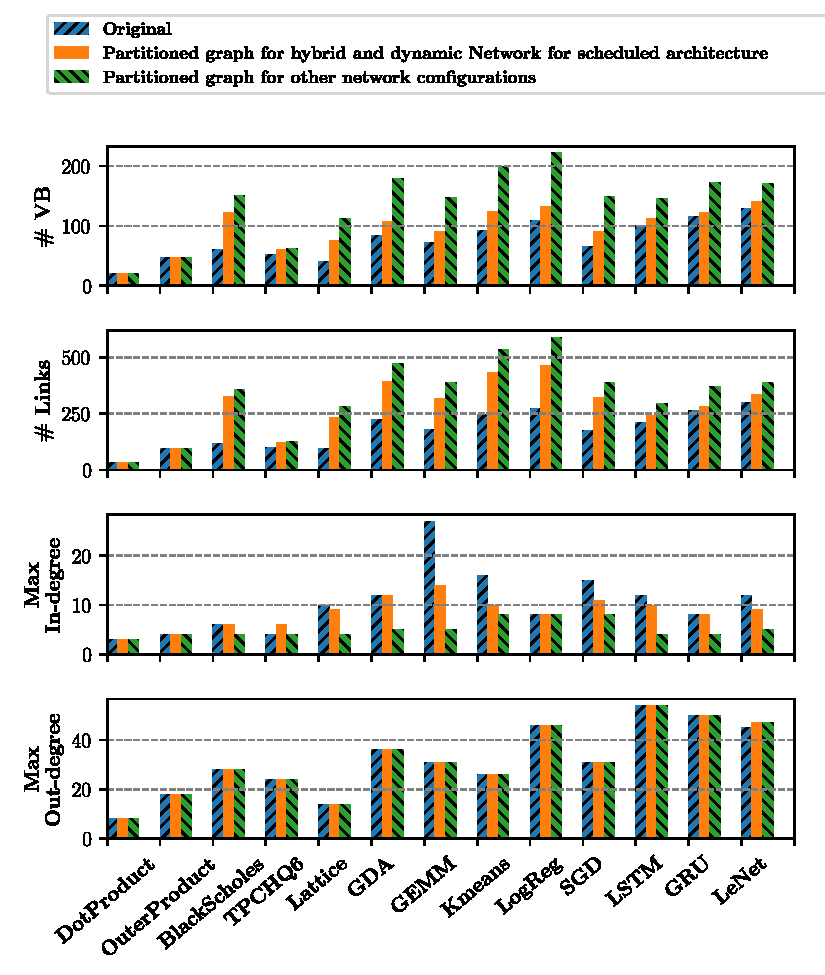
\includegraphics[width=1\columnwidth]{figs/graph.pdf}
\caption{Characteristics of program graphs.}\label{fig:graph}
\end{figure}

We select a mix of applications from domains where hardware accelerators have shown promising performance and energy-efficiency benefits, such as linear algebra, databases, and machine learning.
Table~\ref{tab:benchmark} lists the applications and their data size.
Figure~\ref{fig:util_bw} shows, for each design, which resource limits performance: compute, on-chip memory, or DRAM bandwidth. 
%Variations in these application characteristics introduce different on-chip network requirements.
DotProduct, TPCHQ6, OuterProduct, and BlackScholes are DRAM bandwidth-bound applications. 
These applications use few on-chip resources to achieve maximum performance, resulting in minimal communication.
Lattice (a fast inference model for low-dimensional regression~\cite{garcia2009lattice}), GDA, Kmeans, SGD, and LogReg are compute-intensive applications; for these, maximum performance requires using as much parallelization as possible. 
Finally, LSTM, GRU, and LeNet are applications that are limited by on-chip memory bandwidth or capacity. 
For compute- and memory-intensive applications, high utilization translates to a large interconnection network bandwidth requirement to sustain application throughput. 

Figure~\ref{fig:link}(a,b) shows the communication pattern of applications
characterized on the pipelined CGRA architecture, including the variation in communication granularity. 
Compute and on-chip memory-bound applications show a significant amount of high-bandwidth communication (links with almost 100\% activity). 
A few of these high-bandwidth links also exhibit high broadcast fanout. 
Therefore, a network architecture must provide sufficient bandwidth and efficient broadcasts to sustain program throughput.
On the contrary, time-scheduled architectures, shown in Figure~\ref{fig:link}(c,d), exhibit
lower bandwidth requirements due to the lower throughput of individual compute PBs. 
Even applications limited by on-chip resources have less than a 30\% firing rate on the busiest logical links; this reveals an opportunity for link sharing without sacrificing performance.

Figure~\ref{fig:graph} shows statistics describing the VB dataflow graph before and after partitioning.
The blue bars show the number of VBs, number of logical links, and maximum VB input/output degrees in the original parallelized program; the yellow and green bars show the same statistics after partitioning. 
Fewer VBs are partitioned for hybrid networks and dynamic networks with the time-scheduled architecture, as explained in Section~\ref{sec:partition}. 
The output degree does not change with partitioning because most outputs with a large degree are from broadcast links.

\subsection{Area and Energy Characterization} \label{sec:net_char}

Figure~\ref{fig:sweep} shows that switch and router power scale linearly with the rate of data transmission, but that there is non-zero power at zero-load. 
For simulation, the duty cycle refers to the amount of offered traffic, not accepted traffic.
Because our router uses a crossbar without speedup \cite{dallytowles}, the testbench saturates the router at 60\% duty cycle when providing uniform random traffic. 
Nonetheless, router power still scales linearly with accepted traffic.

A sweep of different switch and router parameters is shown in Figure~\ref{fig:char}. Subplots (d,e,f) show the energy necessary to transmit a single bit through a switch or router.
Subplot (a) shows the roughly quadratic scaling of switch area with the number of links between adjacent switches.
Vector switches scale worse with increasing bandwidth than scalar switches, mostly due to increased crossbar wire load. 
At the same granularity, a router consumes more energy a switch to transmit a single bit of data, even though the overall router consumes less power (as shown in Figure~\ref{fig:sweep}); 
this is because the switch has a higher throughput than the router.
The vector router has lower per-bit energy relative to the scalar router because it can amortize the cost of allocation logic, whereas the vector switch has higher per-bit energy relative to the scalar switch due to increased capacitance in the large crossbar. 
Increasing the number of VCs or buffer depth per VC also significantly increases router area and energy, but reducing the router flit width can significantly reduce router area. 

Overall, these results show that scaling static bandwidth is cheaper than scaling dynamic bandwidth, and a dynamic network with small routers can be used to improve link sharing for low bandwidth communication.  
We also see that a specialized scalar network, built with switches, adds negligible area compared to and is more energy efficient than the vector network. 
Therefore, we use a static scalar network with a bandwidth of 4 for the remainder of our evaluation, except when evaluating the pure dynamic network.
The dynamic network is also optimized for the rare instances when the static scalar network is insufficient. 
When routers transmit scalar data, the high bits of data buffers are clock-gated, reducing energy as shown in (f).
Figure~\ref{fig:area} summarizes the area breakdown of all the network configurations that we evaluate.
\subsection{Network Architecture Exploration} \label{sec:net_dse}

\begin{table}
\footnotesize
\begin{tabular*}{\columnwidth}{p{1cm} p{7cm}}
  \bottomrule
  \textbf{Notation} & \textbf{Description} \\\midrule
  $[$S,H,D$]$ & Static, hybrid, and dynamic network \\\midrule
  x\# & Static bandwidth on vector network (\#links between switches) \\\midrule
  %$s\#$ & Number of links between switches on static scalar network \\\midrule
  f\# & Flit width of a router or vector width of a switch \\\midrule
  v\# & Number of VC in router \\\midrule
  b\# & Number of buffers per VC in router \\\midrule
  $[$db,cd$]$ & Buffered vs. credit-based flow control in switch \\\midrule
  %$[Scheduled, Pipelined]$ & Time scheduled vs deep pipelined accelerator architectures \\\midrule
\end{tabular*}
\caption{Network design parameter summary.}
\label{tab:notation}
\end{table}
\begin{figure}
\centering
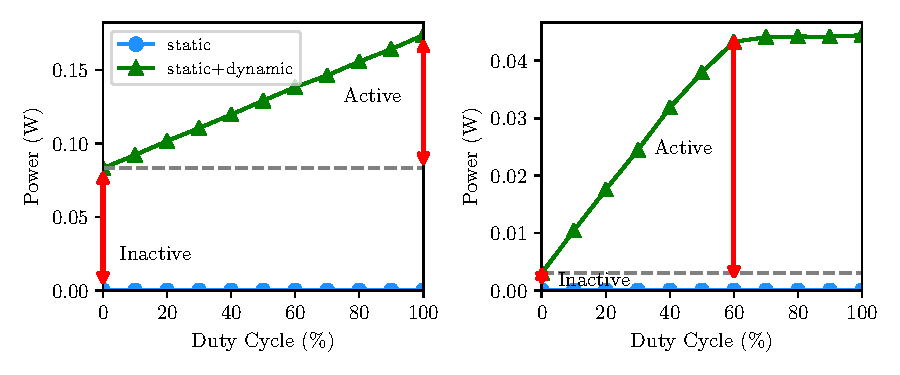
\includegraphics[width=1\columnwidth]{figs/sweep.pdf}
  \caption{Switch and router power with varying duty cycle.}\label{fig:sweep}
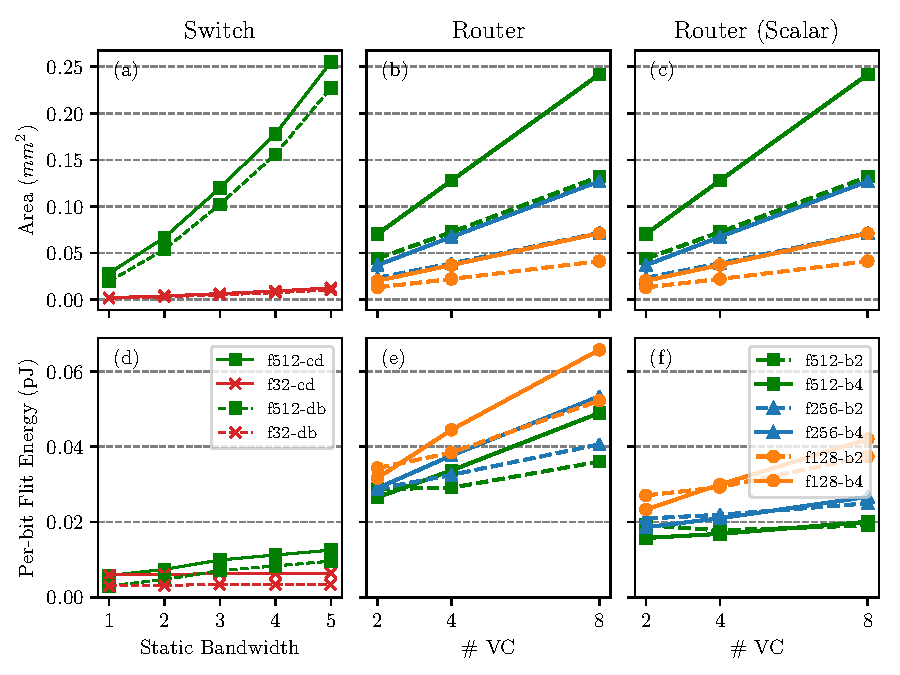
\includegraphics[width=1\columnwidth]{figs/char.pdf}
  \caption{Area and per-bit energy for (a,d) switches and (b,c,e,f) routers. 
  (c,f) Subplots (c,f) show area and energy of the vector router when used for scalar values (32-bit).}\label{fig:char}
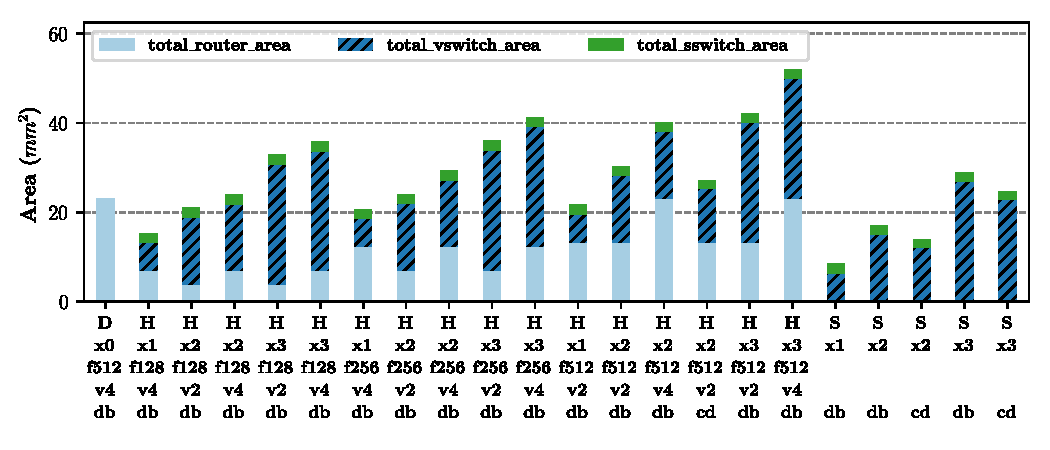
\includegraphics[width=1\columnwidth]{figs/area.pdf}
  \caption{Area breakdown for all network configurations.}\label{fig:area}
\end{figure}

We evaluate our network configurations in five dimensions: performance (perf), performance per network area (perf/area), performance per network
power (perf/watt), network area efficiency (1/area), and network power efficiency (1/power). 
Among these metrics, performance is the most important: networks only consume a small fraction of the overall accelerator area and energy (roughly 10-20\%). 
Because the two key advantages of hardware accelerators are high throughput and low latency, 
we filter out a network design point if it introduces
more than 10\% performance overhead.
This is calculated by comparing to an ideal network with infinite bandwidth and zero latency.

For metrics that are calculated per application, such as performance, performance/watt, and power efficiency, we first normalize the metric with respect to the 
worst network configuration for that application. 
For each network configuration, we present a geometric mean normalized across all applications. 
For all of our experiments, except Section~\ref{sec:scale}, we use a network
size of $14\times14$ end-point PBs. All vector networks use a vectorization factor of 16 (\SI{512}{bit} messages).

\begin{figure}
\centering
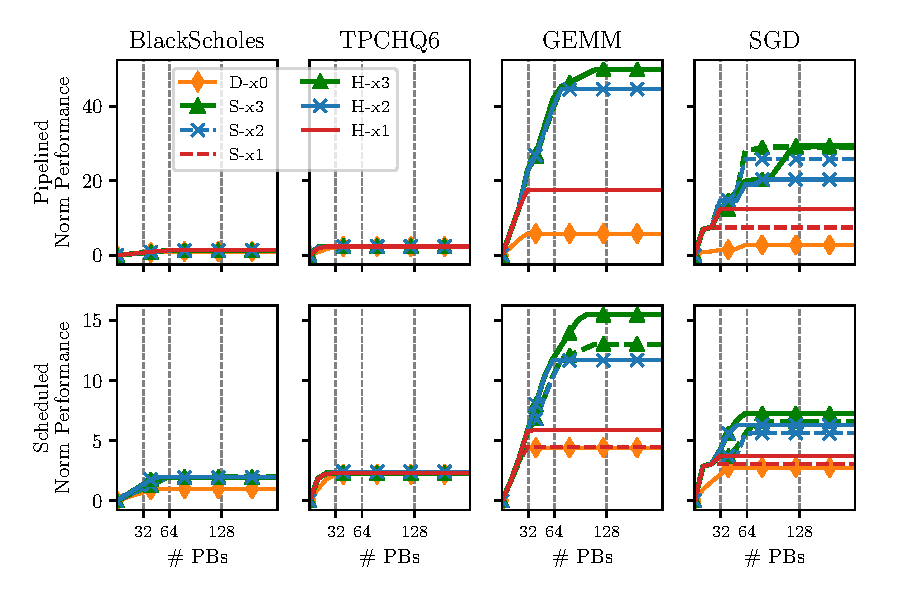
\includegraphics[width=1\columnwidth]{figs/scale.pdf}
\caption{Performance scaling with increased CGRA grid size for different networks.}\label{fig:scale}
\end{figure}
\subsubsection{Bandwidth scaling with network size}\label{sec:scale}
%Figure~\ref{fig:scale} shows the performance scaling of applications as accelerator size scales with different network configurations.
Figure~\ref{fig:scale} shows how different networks allow several applications to scale to different numbers of PBs.
For IO-bound applications (BlackScholes and TPCHQ6), performance does not scale with additional compute and on-chip memory resources.
However, the performance of compute-bound applications (GEMM and SGD) improves with increased resources, but plateaus at a level that is determined by on-chip network bandwidth. 
%Although this is expected for general network designs, it is much more noticeable due to the high-bandwidth communication inherent in pipelined reconfigurable accelerators.
This creates a trade-off in accelerator design between highly vectorized compute PBs with a small network---which would be underutilized for non-vectorized problems---and smaller compute PBs with limited performance due to network overhead. 
For more finely grained compute PBs, both more switches and more costly (higher-radix) switches must be employed to meet application requirements.

The scaling of time-scheduled accelerators (bottom row) is much less dramatic than that of deeply pipelined architectures (top row). 
Although communication between PBs in these architectures is less frequent, the scheduled architecture must use additional parallelization to match the throughput of the pipelined architecture; this translates to larger network sizes. 
%Since scaling dynamic bandwidth is much more expensive than scaling static bandwidth, as shown in section \ref{sec:net_char}, 
%we only explored scaling bandwidth in vector switches. 

For pipelined architectures, both hybrid and static networks provide similar scaling with the same static bandwidth:
the additional bandwidth from the dynamic network in hybrid networks does not provide additional scaling. 
This is mostly due to a bandwidth bottleneck between a PB and its router, which prevents the PB from requesting multiple elements per cycle.
Hybrid networks tend to provide better scaling for time-scheduled architectures; multiple streams can be time multiplexed at each ejection port without losing performance.

\begin{figure}
\centering
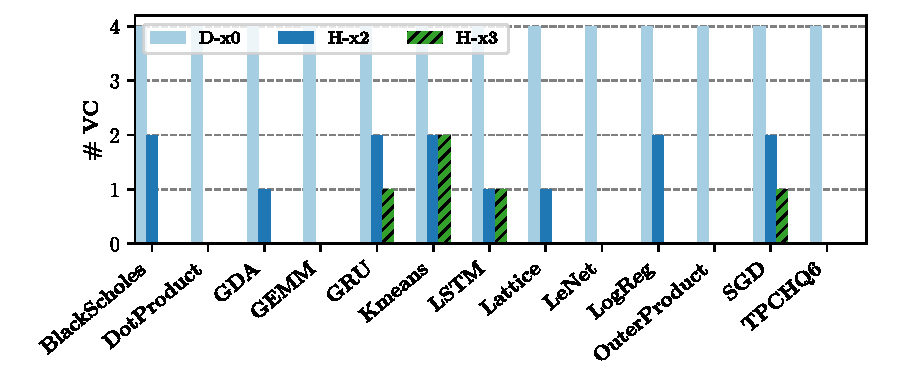
\includegraphics[width=1\columnwidth]{figs/vc.pdf}
  \caption{Number of VCs required for dynamic and hybrid networks. (No VCs indicates that all traffic is mapped to the static network.)}\label{fig:vc}
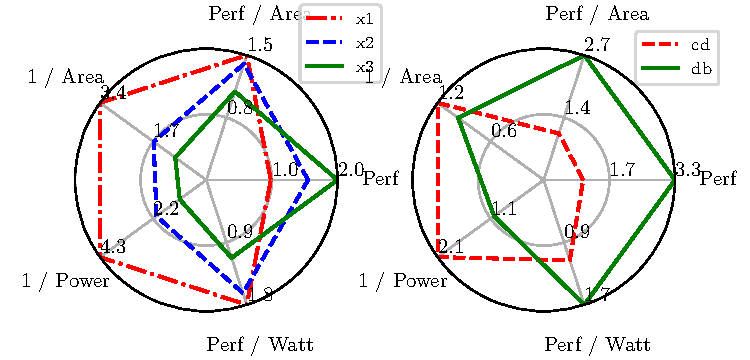
\includegraphics[width=1\columnwidth]{figs/radar_switch.pdf}
  \caption{
    Impact of bandwidth and flow control strategies in switches.}\label{fig:radar_switch}
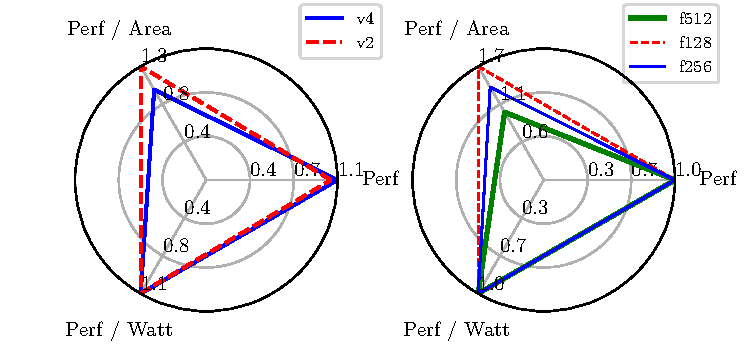
\includegraphics[width=1\columnwidth]{figs/radar_router.pdf}
  \caption{Impact of VC count and flit widths in routers.}\label{fig:radar_router}
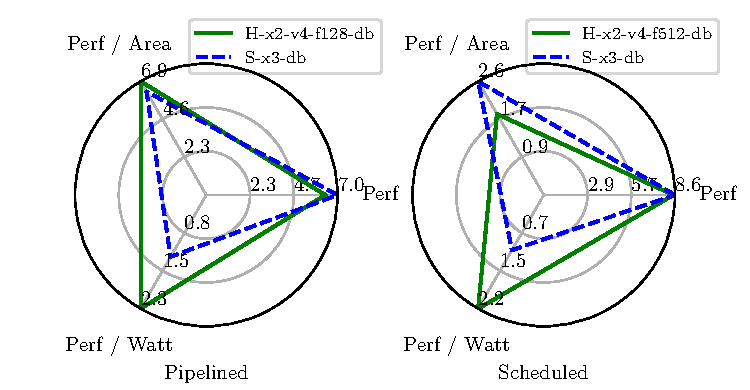
\includegraphics[width=1\columnwidth]{figs/radar_best.pdf}
  \caption{Geometric mean improvement for the best network configurations, relative to the worst configuration.}\label{fig:radar_best}
\end{figure}

\begin{figure*}
\centering
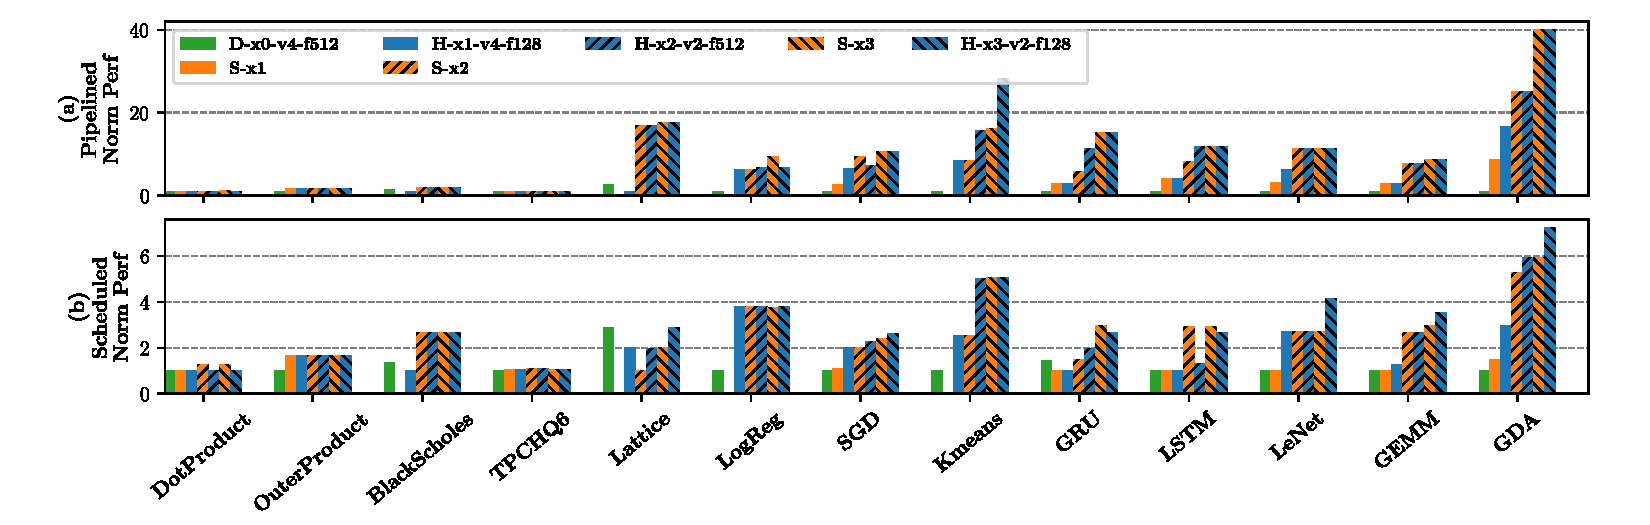
\includegraphics[width=1\linewidth]{figs/perf.pdf}
  \caption{Normalized performance for different network configurations.}\label{fig:perf}
\end{figure*}

\begin{figure}
\centering
  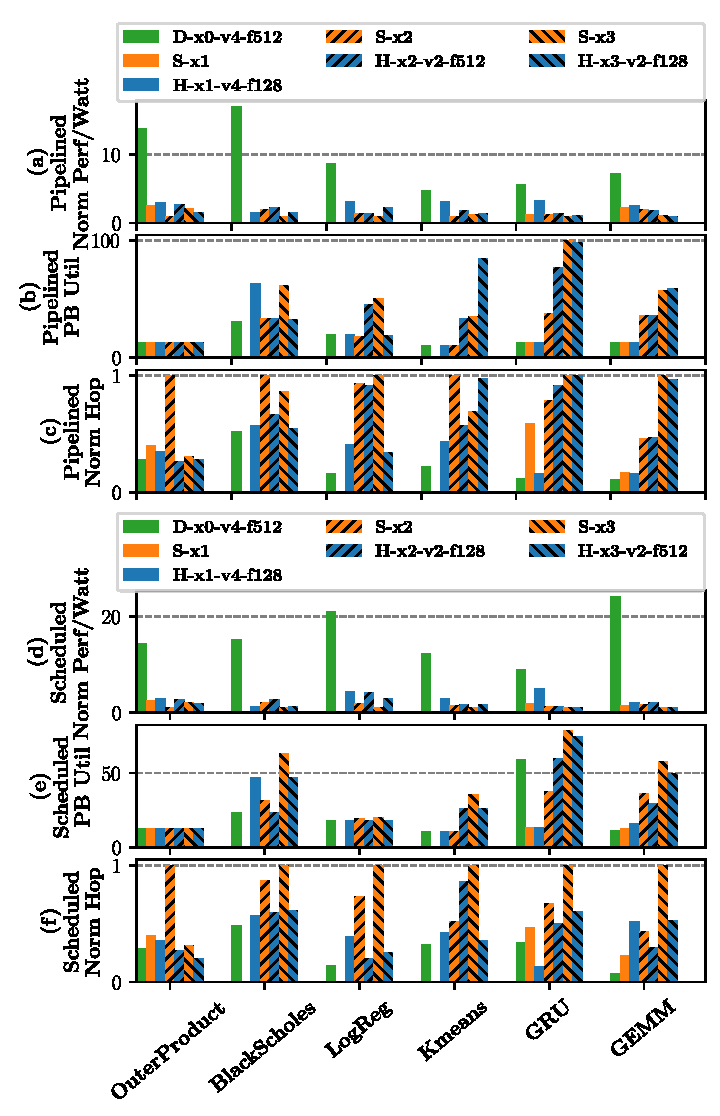
\includegraphics[width=1\columnwidth]{figs/energy.pdf} 
\caption{(a,d): Normalized performance/watt. (b,e): Percentage of compute and memory PBs utilized for each network configuration. 
  (c,f): Total data movement (hop count).}
\label{fig:energy}
\end{figure}

\subsubsection{Bandwidth and flow control in switches}

In this section, we study the impact of static network bandwidth and flow control mechanism (per-hop vs. end-to-end credit-based). 
On the left side of Figure~\ref{fig:radar_switch}, we show that increased static bandwidth results in a linear performance increase and a superlinear increase in area and power. 
As shown in Section~\ref{sec:scale}, any increase in accelerator size must be coupled with increased network bandwidth to effectively scale performance. 
This indicates that network overhead will increase with the size of an accelerator.

The right side of Figure~\ref{fig:radar_switch} shows that, although credit-based flow control reduces the amount of buffering in switches and decreases network area and energy, application performance is significantly impacted. 
This is the result of imbalanced data-flow pipelines in the program: when there are parallel long and short paths over the network, there must be sufficient buffer space on the short path equal to the product of throughput and the difference in latency. 
Because performance is our most important metric, credit-based flow control is not feasible, especially because the impact of bubbles increases with communication distance, and therefore network size.

\subsubsection{VC count and reduced flit width in routers}
In this experiment, we study the area-energy-performance trade-off between routers with different VC counts. As shown
in Section~\ref{sec:net_char}, using many VCs increases both network area and energy.
However, using too few VCs may force roundabout routing on the dynamic network or result in VC allocation failure when the network is heavily utilized.
Nonetheless, the left side of Figure~\ref{fig:radar_router} shows minimal performance improvement from using more VCs. 

Therefore, for each network design, we use a VC count equal to the maximum number of VCs required to map all applications to that network. 
Figure~\ref{fig:vc} shows that the best hybrid network configurations with 2x and 3x static bandwidth require at most 2 VCs, whereas the pure dynamic network requires 4 VCs to map all applications.
%This is different from a traditional processor based (request-response) architecture because, first, less VCs are required to map a large amount of traffic onto dynamic network due deadlock challenges
%specific to streaming architectures, second, communication is much infrequent to incur bandwidth penalty on dynamic network. 
Because dynamic network communication is infrequent, hybrid networks with fewer VCs provide both better energy and area efficiency than networks with more VCs, even though this constrains routing on the dynamic network.
%The improvement is less significant in a time-scheduled architecture because of an overall reduction in required bandwidth.

We also explore the effects of reducing dynamic network bandwidth by using smaller routers;
as shown in Section~\ref{sec:net_char}, routers with smaller flits have a much smaller area.
Ideally, we could scale static network bandwidth while using a low-bandwidth router to provide an escape path and reduce overall area and energy overhead. 
The right side of Figure~\ref{fig:radar_router} shows that, for a hybrid network, reducing flit width improves area efficiency with minimal performance loss. 

%The reduction in performance is more significant in pipelined CGRAs than time-scheduled CGRAs, as the latter has a lower bandwidth requirement.

\subsubsection{Static vs. hybrid vs. dynamic networks}

Figure~\ref{fig:perf} shows the normalized performance for each application running on several network configurations.
%For some applications, the ideal configuration could not be placed and routed onto a static network with 1x bandwidth; missing bars for S-x1 are the result of these failures.
For some applications, the bar for S-x1 is missing; this indicates that place and route failed for all unrolling factors.
For DRAM-bound applications, the performance variation between different networks is trivial because only a small fraction of the network is being used. 
In a few cases (Kmeans and GDA), hybrid networks  provide better performance due to slightly increased bandwidth.
For compute-bound applications, performance primarily correlates with network bandwidth because more bandwidth permits a higher parallelization factor. 

%Figures~\ref{fig:energy} [1,4] show the normalized performance/watt of the network for pipelined and scheduled
%architectures. Figure [2,5] show the corresponding PB utilizations in the network. Figure [3,6] summarize the total
%data movement distributed on static vector, static scalar, dynamic vector and dynamic scalar for that network
%configuration.  
The highest bandwidth static network uses the most PBs, as shown in Figures~\ref{fig:energy}(b,e), because it permits more parallelization. 
It also has more data movement, as shown in (c,f), because PBs can be distributed farther apart. 
Due to bandwidth limitations, low-bandwidth networks perform best with small unrolling factors---they are unable to support the bisection bandwidth of larger program graphs.
This is evident in Figures~\ref{fig:energy}(b,e), where networks D-x0-v4-f512 and S-x2 have small PB utilizations.

With the same static bandwidth, most hybrid networks have better energy efficiency than the corresponding pure static networks, even though routers take more energy than switches to transmit the same amount of data.
This is a result of allowing a small amount of traffic to escape onto the dynamic network: with the dynamic network as a safety net, static place and route tends to converge to better placements with less overall communication.
This can be seen in Figures~\ref{fig:energy}(c,f), where most static networks have larger hop counts than the corresponding hybrid network; hop count is the sum of all runtime link traversals, normalized per-application to the network configuration with the most hops.
Subplots (e,f) show that more PBs are utilized with static networks than hybrid networks.
%Compared to hybrid networks, (e,f), show larger PB utilization at the same parallelization factor on the purely static network .
This is because the compiler imposes less stringent IO constraints on PBs when partitioning for the hybrid network (as explained in Section~\ref{sec:partition}), which results in fewer PBs, less data movement, and greater energy efficiency for hybrid networks.

In Figure~\ref{fig:radar_best}, we summarize the best perf/watt and perf/area (among network configurations with <10\% performance overhead) for pipelined and scheduled CGRA architectures. 
Pure dynamic networks are not shown because they perform poorly due to insufficient bandwidth.
On the pipelined CGRA, the best hybrid network provides a 6.4x performance increase, 2.3x better energy efficiency, and a 6.9x perf/area increase over the worst network configuration. 
The best static network provides 7x better performance, 1.2x better energy efficiency, and 6.3x better perf/area. 
The hybrid network gives the best perf/area and perf/watt, with a small degradation in performance when compared to the static network. 
On the time-scheduled CGRA, both static and hybrid networks have an 8.6x performance improvement. 
The hybrid network gives a higher perf/watt improvement at 2.2x, whereas the static network gives a higher perf/area improvement at 2.6x.
Overall, the hybrid networks deliver better energy efficiency with shorter routing distances by allowing an escape path on the dynamic network.

%It can also provide a decent area efficiency when coupled with a small dynamic network with a minimum performance penalty. 

%\begin{figure}[ht]
%\centering
%\includegraphics[width=\columnwidth]{figs/area.pdf}
%\caption{Area breakdown of network architectures}\label{fig:area}
%\end{figure}

%In this section, we evaluate the proposed network architecture design points from Section~\ref{sec:network}, summarized in Table~\ref{tab:net_dse}.
%Pure dynamic networks are represented with $D{\dash}v0{\dash}s0$, indicating no static links in the network. 
%Pure static networks are prefixed with $v\#{\dash}s\#$, where the $\#$ are number of
%scalar and vector links between switches. Hybrid networks are shown as $D{\dash}v\#{\dash}s\#$.
%Figure~\ref{fig:area_vc} (a) shows the number of VCs required to map each application for architectures containing a dynamic network. 
%%The maximum number of VCs required across all applications is the number of VCs we use to account for area. 
%When computing area for each configuration, we use the maximum number of VCs required to map any application.
%For application in hybrid network with no VCs, all traffic is mapped onto the static network.

%Figure~\ref{fig:area_vc} (b) shows the area breakdown of the architecture. 
%For $D{\dash}v0{\dash}s0$, all links are routed through the dynamic network, resulting in heavy congestion and a large VC requirement. 
%Consequently, the large number of VCs directly contribute to the large router area. 
%All the other dynamic configurations only need 2 VCs to avoid deadlock. 
%The network area contributes only a small fraction of the overall area, but using a dynamic network with a smaller flit width saves router area roughly linearly.
%%The hybrid network $D{\dash}v1{\dash}s4-f512, and D{\dash}v2{\dash}s4-f512$ has slightly larger area than their equivalent bandwidth counterpart design point in static network $v2{\dash}s4$ and $v3{\dash}s4$ due to the overhead on dynamic routing and buffering. 

%Figure~\ref{fig:slow_down} (a) shows the performance degradation normalized to the ideal network with infinite buffers; all the other design points have an end-point buffer with depth 4 inside the CUs.
%We found that for memory bandwidth bound applications, the performance is roughly the same across all design points, mostly due to the low CU utilization and lack of congestion. 
%Although BlackScholes is DRAM bandwidth bound, the inner loop partition introduces lots of CUs communicating their temporary results. 
%The slow-down with BlackScholes with static network compared to ideal network is due to the pipeline bubbles introduced by VB partitioning as explained in Section \ref{sec:network}. 

%Overall, the hybrid network with the $v1$ static network has a slowdown of less than 2x overall, while the hybrid network with $v2$ has static-equivalent performance.

%The static network with credit-based flow control suffers from insufficient end-point buffers for most applications, resulting in poor performance. 
%The slowdown in dynamic and hybrid networks is mostly due to the high-throughput broadcasts and congestion. 
%Figure~\ref{fig:slow_down} (b) shows the slowdown normalized to total area. 
%Since the network only takes a small fraction of the chip area, the trends is similar to performance. 

%Figure~\ref{fig:slow_down}(c) shows the network energy normalized to $v2{\dash}s4$. 
%The pure dynamic network consumes the most energy because of the amount of buffers and the router's inherently higher per-flit energy. 
%Breaking down the hybrid network energy, we can see that vast majority of communication is mapped to the static network. 
%There is a small gap between energy on $v2{\dash}s4$ and $D{\dash}v2{\dash}s4$, where the hybrid consumes less energy, even though all traffic is mapped onto the static network. 
%Another outlier on LeNet $D{\dash}v2{\dash}s4$ consumes more energy then $v2{\dash}s4{\dash}db$ is likely introduced by randomness from the iterative placer. 
%These are discrepancies introduced by different placements having different distances between nodes.
%It is also important to note hat the overprovisioned static capacity has a high (31\%) mean energy cost, even though it is not being used.
%%This is due to a limitation in current implementation that pure static networks are placed and routed with only back tracking placer, while the hybrid is also using the iterative placer. 
%%As a result, we found better mapping on hybrid network which reduce the hop distance on links, which is not essential for slowdown but directly translates into energy. 
%%However, in theory we should be able to use both algorithm on all design points. 

%In Figure~\ref{fig:slow_down} (d), we show the normalized power. 
%Here, design points with large slowdown naturally have lower power, such as $v3{\dash}s4{\dash}cd$. 
%However, we also show that the network is consuming only a very small portion of the power compared with the compute tiles. 
%The network only consumes around 0--3 W of energy compared to the theoretical peak Plasticine power of 49W.
%Therefore, among the metrics of performance, area, and power, performance is the most important metric to measure the network architectures. 

%%
%%This allows it to be stored in the smaller buffers without any translation logic, and does not result in a loss of throughput (the throughput would be limited regardless at the non-priority VC).
%%Because the priority VC is considered in route scoring, the placer is able to ensure that less than 1\% of traffic in the worst app (XXX) traverses non-priority VCs.
%%This scheme results in a XXX\% lower network area, with a geometric mean slowdown of XXX\% (worst XXX\%).

\section{Related Work}
\label{relatedWork}
%\christos{this is quite long. you should trim it a little. First, it is not criteria, it is requirements right? Once you establish the criteria, you should be able to trim the text as you can quickly mention why each architecture fails some criteria. E.g., GPUs are easy to take down in 1-2 sentences (instruction overheads).}

%\christos{One obvious question is how did you pick these archs to list in table 1? Twist a little the first sentence of each paragraph to mention that what class of archs the ones you mention represent (so that the reader can cast similar archs to this paragraph). Also mention somewhere in the text that there are numerous archs and you will discuss representative archs from each major class}

%\christos{At the end of this section I am in page 4 and I still don't ahve an intuition of what is the key to fix to get fast compilation. This is important, bring it up earlier (intro?)}

%
%We identify the following criteria to achieve the aforementioned goals of flexibility, efficiency,
%and programmability:
Table~\ref{t:requirements} introduced key architectural features required to efficiently execute parallel patterns.
We now discuss the significant related work in light of these features.

{\bf Reconfigurable scratchpads:} Several of the previously proposed reconfigurable fabrics lack support for reconfigurable, distributed scratchpad memories.  Without the ability to reconfigure the on-chip memory system with the different banking and buffering strategies needed to support parallel patterns, the memory system becomes the bottleneck for many workloads.

For example, ADRES~\cite{adres}, DySER~\cite{dyser}, Garp~\cite{garp}, and Tartan~\cite{tartan} closely couple a reconfigurable fabric with a CPU. These architectures access main memory through the cache hierarchy shared with the host CPU. ADRES and DySER tightly integrate the reconfigurable fabric into the execution stage of the processor pipeline, and hence depend on the processor's load/store unit for memory accesses. ADRES consists of a network of functional units, reconfigurable elements with register files, and a shared multi-ported register file.
%However, exploiting nested parallelism is hard due to memory access serialization at the cache hierarchy.
DySER is a reconfigurable array with a statically configured interconnect designed to execute innermost loop bodies in a pipelined fashion. However, dataflow graphs with back-edges or feedback paths are not supported, which makes it challenging to execute patterns such as \emph{Fold} and nested parallel patterns.  Garp consists of a MIPS CPU core and an FPGA-like coprocessor. The bit-level static interconnect of the co-processor incurs the same reconfiguration overheads as a traditional FPGA, restricting compute density.
%the absence of distributed scratchpads makes exploiting nested parallelism difficult.
Piperench~\cite{piperench} consists of a pipelined sequence of ``stripes'' of functional units (FUs).  A word-level crossbar separates each stripe. Each FU has an associated register file which holds temporary results.  Tartan consists of a RISC core and an asynchronous, coarse-grained reconfigurable fabric (RF).  The RF architecture is hierarchical with a dynamic interconnect at the topmost level, and a static interconnect in the inner level. The architecture of the innermost RF core is modeled after Piperench~\cite{piperench}.


%\gist{adres: Network of functional units and reconfigurable elements with a multi-ported register file with a memory hierarchy. The core can be configured
%  to operate either as a VLIW core or a reconfigurable matrix. Exploits loop-level parallelism but only at innermost level~\cite{dresc}. Exploiting nested
%  parallelism is hard as access to intermediate data structures will be serialized through the memory hierarchy.}

%\gist{dyser: Array of reconfigurable functional units in a statically programmable interconnect, part of the execute stage of a processor pipeline.
%  Credit-based flow control presumably uses a separate interconnect path, giving benefit of doubt.
%  No explicit scratchpads, hence relies on the processor's cache hierarchy to capture locality. Nested parallelism not exploited because
%DySER does not support executing dataflow graphs with back-edges.}

%\gist{garp: Hybrid architecture with a MIPS CPU and Reconfigurable FPGA-like co-processor with bit-level interconnect. Data locality captured with CPU's cache hierarchy
%  and memory queues for sequential accesses. With the absence of scratchpad memories, cannot support exploiting nested
%  parallelism as intermediate data structures have to go to the memory hierarchy.}

%\gist{piperench: Coprocessor with a sequence of pipeline "stripes" of FUs connected with a word-level crossbar. Lack of scratchpad memories
%and the fact that the compiler unrolls all loops during compilation means that nested parallelism is not exploited.}
%
%\gist{tartan: Hybrid architecture with RISC CPU and clockless reconfigurable fabric (RF) as a peer-processor. Aimed to be general purpose.
%  RF is hierarchical with a Piperench-style core at the innermost level. No scratchpads, locality is captured via a memory hierarchy shared with CPU.
%  Exploiting nested parallelism is hard because of absence of scratchpads, need to go through top-level dynamic interconnect to access memories.
%  Successive pipeline stages in a \emph{page} separated a partial crossbar, which provides flexibility but also incurs area
%and power overhead.}
{\bf Reconfigurable datapaths} Architectures with reconfigurable functional units consume less power
    as they do not incur the overheads of traditional instruction pipelines such as instruction fetch, decode, and register file access.
    These overheads account for about 40\% of the datapath energy on the CPU~\cite{inefficiencies} and about 30\%
    of the total dynamic power on the GPU~\cite{gpuwattch}. Furthermore, using a reconfigurable datapath in place of a
    conventional instruction pipeline in a GPU reduces energy consumption by about 57\%~\cite{sgmf}.
		The Raw microprocessor~\cite{raw} is a tiled architecture where each tile consists of a single-issue in-order processor, a floating point
		unit, a data cache, and a software-managed instruction cache. Tiles communicate with their nearest neighbors using pipelined, word-level static and dynamic
		networks. Plasticine does not incur the overheads of dynamic networks and general purpose processors mentioned above. Using hardware managed caches
		in place of reconfigurable scratchpads reduces power and area efficiency in favor of generality.

{ \bf Dense datapaths and hierarchical pipelines:} Plasticine's hierarchical architecture, with dense pockets of pipelined SIMD functional units and decentralized control,
enables capturing a substantial amount of data communication within PCUs and efficiently exploiting coarse-grained pipeline parallelism in applications.
In contrast, architectures that lack hierarchal support for nested pipelining in the architecture use their global interconnect to communicate most results.
Hence, the interconnect can be a bandwidth, power, or area bottleneck.
For example, RaPiD~\cite{rapid} is a one-dimensional array of ALUs, registers, and memories with hardware support for static and dynamic control.
A subsequent research project called Mosaic~\cite{staticVsScheduled} includes a static hybrid interconnect along with hardware support to switch
between multiple interconnect configurations. RaPiD's linear pipeline enforces a rigid control flow which makes it difficult to exploit nested parallelism.
HRL~\cite{hrl} combines coarse-grained and fine-grained logic blocks with a hybrid static interconnect. While a centralized scratchpad enables some on-chip buffering,
the architecture is primarily designed for memory-intensive applications with little locality and nested parallelism.
Triggered instructions~\cite{ti} is an architecture consisting of coarse-grained processing elements (PEs) of ALUs and registers in a static interconnect.
Each PE contains a scheduler and a predicate register to implement dataflow execution using triggers and guarded actions. The control flow mechanism used in Plasticine
has some similarities with Triggered instructions. While this architecture has the flexibility to exploit nested parallelism and locality, the lack of hierarchy increases
communication over the global interconnect which can create bottlenecks, and reduces compute density in the datapath.

% \gist{rapid: One-dimensional array of ALUs, registers, and memories with hardware support for static and dynamic control.  The linear pipeline makes it hard to exploit nested parallelism. Applications written in RaPiD's programming environment, RaPiD-C, are not completely abstracted away from low-level hardware details as the RaPiD-C specification close to the structural description of the algorithm~\cite{rapidc}.}

%\gist{hrl: combines coarse-grained and fine-grained logic blocks with a hybrid static interconnect. While a centralized
% scratchpad enables some on-chip buffering, the architecture is
% primarily designed for memory-intensive applications with little locality and nested parallelism. Programming HRL leverages
% Verilog generated from Vivado HLS~\cite{vivadohls} and conventional plas-and-route.}
%{\bf Support for scatter-gather:} Plasticine uses configurable address generators along with address coalescing that allows for efficient use of off-chip memory bandwidth. 
%\gist{Triggered instructions: Spatial accelerator with triggers and guarded actions to control execution flow.
%  The architecture has the flexibility to exploit nested parallelism and provides scratchpads to exploit locality.
%  However, parallel execution across PEs requires constant communication over interconnect switches which
%  can be power inefficient. Plasticine has much higher compute density with dense pockets of pipelined SIMD functional units.
%  Also, the lack of a high-level compiler means that mapping applications is a tedious manual process of speficying all low-level details.}

%\gist{Focus of this paper is spatial architectures, evaluation against GPGPU is out of scope of this paper.
%  From the architectures in Table~\ref{t-related}, the only
%  other spatial architecture that supports a high-level programming interface and which is capable of mapping
%  entire applications with nested parallelism and custom on-chip data structures is the FPGA.
%  As a result, we evaluate our architecture and compiler against the FPGA in~\ref{evaluation}.
%}

%
%\begin{itemize}
%  \item \emph{Coarse-grained Reconfigurable datapath}: Accelerators designed with a datapath containing reconfigurable functional units consume less power
%    as they do not incur the overheads of traditional instruction pipelines such as instruction fetch, decode, and register file access.
%    These overheads account for about 40\% of the datapath energy on the CPU~\cite{inefficiencies} and about 30\%
%    of the total dynamic power on the GPU~\cite{gpuwattch}. Furthermore, using a reconfigurable datapath in place of a
%    conventional instruction pipeline in a GPU reduces energy consumption by about 57\%~\cite{sgmf}.
%    Coarse-grained reconfigurable units provide higher area and power efficiency over fine-grained units
%    by increasing compute density and amortizing the cost of reconfiguration overheads.
%  \item \emph{Local, distributed scratchpad memories}: Off-chip DRAM accesses consume a couple of orders of magnitude
%    more energy compared to on-chip memory accesses~\cite{horowitz_isscc14}. On-chip scratchpad memories provide explicit means
%    to exploit data locality in applications having different kinds of access patterns. Further, scratchpads need to be distributed to
%    enable data structure banking and parallel access to independent data structures. Such high bandwidth parallel access is
%    required to match compute parallelism and sustain high throughput within the compute pipeline.
%  \item \emph{Exploit nested parallelism}: Applications that benefit from hardware acceleration tend to
%    exhibit multiple types of data parallelism~\cite{delite-tecs14}, often at multiple levels of nesting~\cite{rodinia}.
%    Accelerators must support efficient mapping such hierarchically parallel datapaths while incurring minimal overhead.
%  \item \emph{Static hybrid interconnect}: Static
%      bit-level interconnect incurs a lot of area overhead and scales poorly with number of bits~\cite{fpgaSurvey, calhoun, bolsens}.
%      Static interconnect that connects busses of wires improves interconnect area~\cite{busInterconnect}, as the configuration for the
%      switches can be amortized over the bus width. Additionally, using a bit-level control interconnect to handle control logic greatly
%      improves interconnect utilization and power consumption~\cite{staticVsScheduled, hrl} as the data and control do not have to be
%      packed into the same bus.
%\end{itemize}
%
% \begin{table*}[]
% \centering
% \caption{Table of previous work in relation to the criteria outlined above.}
% \label{t-related}
% \resizebox{\textwidth}{!}{%
% \begin{tabular}{@{}llccccccccccccc@{}}
% \bottomrule
% %                                       & \multicolumn{3}{c}{Instruction Stream} & \multicolumn{5}{c}{Tightly Coupled Configurations}                                                & \multicolumn{4}{c}{Loosely Coupled Configurations} &                    \\
% Feature                                &\emph{Goal}                                                                   & ADRES~\cite{adres} & DySER~\cite{dyser}   & Garp~\cite{garp}  & PipeRench~\cite{piperench}  & Tartan~\cite{tartan}  & RaPiD~\cite{rapid} & HRL~\cite{hrl} &\begin{tabular}[c]{@{}l@{}}Triggered\\ Instructions\end{tabular}~\cite{ti}  & FPGA      & \textbf{This Work} \\ \midrule
% Coarse-grained Reconfigurable Datapath &\begin{tabular}[c]{@{}l@{}}\emph{Efficiency}\\\emph{Flexibility}\end{tabular} &\tick               & \tick                &\x                 &  \tick                      &\tick                  & \tick              &\tick           &             \tick                                                          & \x        & \tick              \\ \midrule
% Exploit nested parallelism             &\emph{Flexibility}                                                            &\x                  & \x                   &\x                 &  \x                         & \x                    & \x                 & \x             &             \tick                                                          & \tick     & \tick              \\ \midrule
% Local, distributed scratchpad memories &\emph{Efficiency}                                                             &\x                  & \x                   &\x                 &  \x                         &\x                     & \tick              & \x             &             \tick                                                          &\tick      & \tick              \\ \midrule
% Static hybrid interconnect             &\emph{Efficiency}                                                             &\x                  & \tick                &\x                 &  \x                         & \x                    & \tick              &\tick           &             \tick                                                          &  \x       & \tick              \\ \midrule
% High-level programming interface       &\emph{Programmability}                                                        &\tick               & \ytick               &\ytick             &  \ytick                     & \ytick                & \x                 & \x             &             \x                                                             &\tick      & \tick              \\ \midrule
% Fast Compilation                       &\emph{Programmability}                                                        &\tick               & \tick                & \tick             &  \tick                      & \tick                 & ?                  & \x             &             \x                                                             &  \x       & \tick              \\ \bottomrule
% \end{tabular}
% }
% \end{table*}

%One of the most successful accelerator architectures is the GPGPU~\cite{gpu}, which provides massive parallel processing
%capabilities with thousands of simultaneously active thread contexts. While some form of nested parallelism and locality can be exploited
%multiple SMs and scratchpads respectively, GPGPUs follow a conventional instruction stream execution model and hence
%incurs associated overheads~\cite{gpuwattch, sgmf}. Additionally, inter-SM communication can only happen via global memory,
%which makes it hard to exploit coarse-grained pipeline parallelism across SMs efficiently.

%Wavescalar is a dynamic dataflow architecture with four pipeline stages with broadcast and dynamic
%interconnects. While nested parallelism can potentially be exploited with multi-threaded support, lack of a distributed scratchpad means
%that parallel independent memory accesses are serialized at the shared memory interface. A TRIPS core is a grid of execution nodes,
%where each node has an ALU and a reservation station. Execution of a hyperblock proceeds in dataflow fashion, where the output of one node
%is directly forwarded to the reservation stations of dependent nodes. However, the inter-node interconnect is not statically reconfigurable.
%\gist{wavescalar: Dynamic dataflow architecture with five stages: Input, match, dispatch, execute. While execution is dataflow driven, the
%  datapath is not reconfigurable. Broadcast and dynamic interconnects used. Coarse-grained parallelism can be exploited using multi-threaded
%  support and barriers. However, lack of a distributed scratchpad means that parallel memory accesses are serialzied at the memory interface.}

%A large body of previous work exists on architectures and tools for coarse-grained reconfigurable architectures~\cite{cgraSurvey1, cgraSurvey2}.
%We compare and contrast the several related works in relation to the criteria above in Table~\ref{t-related}.

%\gist{trips: Grid of execution cores, where each core has an ALU and a reservation station. Supports different modes to exploit ILP,
%  DLP, TLP. Dataflow driven execution, but datapath and inter-node interconnect is not statically reconfigurable.}



\chapter{Conclusions (WIP)} \label{sec:conclusion}

Reconfigurable dataflow accelerators (RDAs) are a promising class of spatial accelerators, which deliver higher performance-to-resource efficiency than conventional process architectures while capturing a large application space.
However, to sustain these benefits as RDAs get larger, the software stack must address the challenges of (a) distributed control / correctness and (b) efficient resource allocation.

We address these challenges by proposing a distributed asynchronous control scheme and a program decomposition method. 
We develop a compiler, \name{}, that constructs a virtual block dataflow graph (VBDFG) from a program specification and generates a minimal set of peer-to-peer synchronizations, which allow fine-grained parallelization factors that would otherwise incur large communication overheads.
Furthermore, operations on VBDFG are decomposed and assigned to a heterogenous collections of physical blocks (PBs). 
Lastly, we implement these techniques and through evaluations show that \name{} achieves a speedup of 4x over a Tesla V100 GPU.
We hope that the approach and implementation presented in this work will help scale modern RDAs add a steady pace..

We show that the best network design depends on both applications and the underlying accelerator architecture.
Network performance correlates strongly with bandwidth for streaming accelerators, and scaling raw bandwidth is more area- and energy-efficient with a static network.
We show that the application mapping can be optimized to move less data by using a dynamic network as a fallback from a high-bandwidth static network.
%this contributes a 6.9x average performance per area and 2.3x average energy-efficiency improvement for a static-dynamic hybrid network.
This static-dynamic hybrid network provides a 1.8x energy-efficiency and
2.8x performance advantage over the purely static and purely dynamic networks, respectively.
  %Furthermore, we show that spatial architectures require larger switches as programs get bigger, imposing super-linear scaling of network size with chip area.





\section*{Acknowledgments}
\label{acknowledgements}
The authors thank Tony Wu for his assistance with this paper, 
and the reviewers for their suggestions.
This work is supported by DARPA 
Contract-Air Force FA8750-12-2-0335;
Army Contracts FA8750-14-2-0240 and FA8750-12-20335;
NSF Grants CCF-1111943 and IIS-1247701.
The views and conclusions contained herein are those
of the authors and should not be interpreted as necessarily
representing the official policies or endorsements, either expressed or implied, of DARPA or the U.S. Government.

%\def\bibliofont{\fontsize{6}{7}}
%\def\bibfont{\fontsize{6}{7}}

\def\bibliofont{\scriptsize}
%\def\bibfont{\scriptsize}
\renewcommand{\bibfont}{\fontsize{6.46pt}{6.46pt}\selectfont} %\scriptsize}


\pagebreak
\bibliographystyle{ACM-Reference-Format}
%\bibliography{references}

\fontsize{8}{9}{
%%% -*-BibTeX-*-
%%% Do NOT edit. File created by BibTeX with style
%%% ACM-Reference-Format-Journals [18-Jan-2012].

\begin{thebibliography}{00}

%%% ====================================================================
%%% NOTE TO THE USER: you can override these defaults by providing
%%% customized versions of any of these macros before the \bibliography
%%% command.  Each of them MUST provide its own final punctuation,
%%% except for \shownote{}, \showDOI{}, and \showURL{}.  The latter two
%%% do not use final punctuation, in order to avoid confusing it with
%%% the Web address.
%%%
%%% To suppress output of a particular field, define its macro to expand
%%% to an empty string, or better, \unskip, like this:
%%%
%%% \newcommand{\showDOI}[1]{\unskip}   % LaTeX syntax
%%%
%%% \def \showDOI #1{\unskip}           % plain TeX syntax
%%%
%%% ====================================================================

\ifx \showCODEN    \undefined \def \showCODEN     #1{\unskip}     \fi
\ifx \showDOI      \undefined \def \showDOI       #1{#1}\fi
\ifx \showISBNx    \undefined \def \showISBNx     #1{\unskip}     \fi
\ifx \showISBNxiii \undefined \def \showISBNxiii  #1{\unskip}     \fi
\ifx \showISSN     \undefined \def \showISSN      #1{\unskip}     \fi
\ifx \showLCCN     \undefined \def \showLCCN      #1{\unskip}     \fi
\ifx \shownote     \undefined \def \shownote      #1{#1}          \fi
\ifx \showarticletitle \undefined \def \showarticletitle #1{#1}   \fi
\ifx \showURL      \undefined \def \showURL       {\relax}        \fi
% The following commands are used for tagged output and should be
% invisible to TeX
\providecommand\bibfield[2]{#2}
\providecommand\bibinfo[2]{#2}
\providecommand\natexlab[1]{#1}
\providecommand\showeprint[2][]{arXiv:#2}

\bibitem[\protect\citeauthoryear{Auerbach, Bacon, Cheng, and Rabbah}{Auerbach
  et~al\mbox{.}}{2010}]%
        {auerbach10lime}
\bibfield{author}{\bibinfo{person}{Joshua Auerbach}, \bibinfo{person}{David~F.
  Bacon}, \bibinfo{person}{Perry Cheng}, {and} \bibinfo{person}{Rodric
  Rabbah}.} \bibinfo{year}{2010}\natexlab{}.
\newblock \showarticletitle{Lime: A Java-compatible and Synthesizable Language
  for Heterogeneous Architectures}. In \bibinfo{booktitle}{{\em Proceedings of
  the ACM International Conference on Object Oriented Programming Systems
  Languages and Applications}} {\em (\bibinfo{series}{OOPSLA})}.
  \bibinfo{pages}{89--108}.
\newblock
\showISBNx{978-1-4503-0203-6}
\showDOI{%
\url{https://doi.org/10.1145/1869459.1869469}}


\bibitem[\protect\citeauthoryear{Bachrach, Vo, Richards, Lee, Waterman,
  Avizienis, Wawrzynek, and Asanovic}{Bachrach et~al\mbox{.}}{2012}]%
        {chisel}
\bibfield{author}{\bibinfo{person}{Jonathan. Bachrach}, \bibinfo{person}{Huy
  Vo}, \bibinfo{person}{Brian Richards}, \bibinfo{person}{Yunsup Lee},
  \bibinfo{person}{Andrew Waterman}, \bibinfo{person}{Rimas Avizienis},
  \bibinfo{person}{John Wawrzynek}, {and} \bibinfo{person}{Krste Asanovic}.}
  \bibinfo{year}{2012}\natexlab{}.
\newblock \showarticletitle{Chisel: Constructing hardware in a Scala embedded
  language}. In \bibinfo{booktitle}{{\em Design Automation Conference (DAC),
  2012 49th ACM/EDAC/IEEE}}. \bibinfo{pages}{1212--1221}.
\newblock
\showISSN{0738-100X}


\bibitem[\protect\citeauthoryear{Bacon, Rabbah, and Shukla}{Bacon
  et~al\mbox{.}}{2013}]%
        {fpgaProgramming}
\bibfield{author}{\bibinfo{person}{David Bacon}, \bibinfo{person}{Rodric
  Rabbah}, {and} \bibinfo{person}{Sunil Shukla}.}
  \bibinfo{year}{2013}\natexlab{}.
\newblock \showarticletitle{FPGA Programming for the Masses}.
\newblock \bibinfo{journal}{{\em Queue\/}} \bibinfo{volume}{11},
  \bibinfo{number}{2}, Article \bibinfo{articleno}{40} (\bibinfo{date}{Feb.}
  \bibinfo{year}{2013}), \bibinfo{numpages}{13}~pages.
\newblock
\showISSN{1542-7730}
\showDOI{%
\url{https://doi.org/10.1145/2436696.2443836}}


\bibitem[\protect\citeauthoryear{Bolsens}{Bolsens}{2006}]%
        {bolsens}
\bibfield{author}{\bibinfo{person}{Ivo Bolsens}.}
  \bibinfo{year}{2006}\natexlab{}.
\newblock \bibinfo{title}{Programming Modern FPGAs, International Forum on
  Embedded Multiprocessor SoC, Keynote,}.
\newblock
  \bibinfo{howpublished}{\url{http://www.xilinx.com/univ/mpsoc2006keynote.pdf}}.
\newblock


\bibitem[\protect\citeauthoryear{Calhoun, Ryan, Khanna, Putic, and
  Lach}{Calhoun et~al\mbox{.}}{2010}]%
        {calhoun}
\bibfield{author}{\bibinfo{person}{Benton.~Highsmith Calhoun},
  \bibinfo{person}{Joseph~F. Ryan}, \bibinfo{person}{Sudhanshu Khanna},
  \bibinfo{person}{Mateja Putic}, {and} \bibinfo{person}{John Lach}.}
  \bibinfo{year}{2010}\natexlab{}.
\newblock \showarticletitle{Flexible Circuits and Architectures for Ultralow
  Power}.
\newblock \bibinfo{journal}{{\it Proc. IEEE}} \bibinfo{volume}{98},
  \bibinfo{number}{2} (\bibinfo{date}{Feb} \bibinfo{year}{2010}),
  \bibinfo{pages}{267--282}.
\newblock
\showISSN{0018-9219}
\showDOI{%
\url{https://doi.org/10.1109/JPROC.2009.2037211}}


\bibitem[\protect\citeauthoryear{Callahan, Hauser, and Wawrzynek}{Callahan
  et~al\mbox{.}}{2000}]%
        {garp}
\bibfield{author}{\bibinfo{person}{Timothy~J. Callahan},
  \bibinfo{person}{John~R. Hauser}, {and} \bibinfo{person}{John Wawrzynek}.}
  \bibinfo{year}{2000}\natexlab{}.
\newblock \showarticletitle{The Garp architecture and C compiler}.
\newblock \bibinfo{journal}{{\em Computer\/}} \bibinfo{volume}{33},
  \bibinfo{number}{4} (\bibinfo{date}{Apr} \bibinfo{year}{2000}),
  \bibinfo{pages}{62--69}.
\newblock
\showISSN{0018-9162}
\showDOI{%
\url{https://doi.org/10.1109/2.839323}}


\bibitem[\protect\citeauthoryear{Casper and Olukotun}{Casper and
  Olukotun}{2014}]%
        {casper}
\bibfield{author}{\bibinfo{person}{Jared Casper} {and} \bibinfo{person}{Kunle
  Olukotun}.} \bibinfo{year}{2014}\natexlab{}.
\newblock \showarticletitle{Hardware Acceleration of Database Operations}. In
  \bibinfo{booktitle}{{\em Proceedings of the 2014 ACM/SIGDA International
  Symposium on Field-programmable Gate Arrays}} {\em (\bibinfo{series}{FPGA
  '14})}. \bibinfo{publisher}{ACM}, \bibinfo{address}{New York, NY, USA},
  \bibinfo{pages}{151--160}.
\newblock
\showISBNx{978-1-4503-2671-1}
\showDOI{%
\url{https://doi.org/10.1145/2554688.2554787}}


\bibitem[\protect\citeauthoryear{Catanzaro, Garland, and Keutzer}{Catanzaro
  et~al\mbox{.}}{2011}]%
        {catanzaro11copperhead}
\bibfield{author}{\bibinfo{person}{Bryan Catanzaro}, \bibinfo{person}{Michael
  Garland}, {and} \bibinfo{person}{Kurt Keutzer}.}
  \bibinfo{year}{2011}\natexlab{}.
\newblock \showarticletitle{Copperhead: compiling an embedded data parallel
  language}. In \bibinfo{booktitle}{{\em Proceedings of the 16th ACM symposium
  on Principles and practice of parallel programming}} {\em
  (\bibinfo{series}{PPoPP})}. \bibinfo{publisher}{ACM}, \bibinfo{address}{New
  York, NY, USA}, \bibinfo{pages}{47--56}.
\newblock
\showISBNx{978-1-4503-0119-0}
\showDOI{%
\url{https://doi.org/10.1145/1941553.1941562}}


\bibitem[\protect\citeauthoryear{Chen, Luo, Liu, Zhang, He, Wang, Li, Chen, Xu,
  Sun, and Temam}{Chen et~al\mbox{.}}{2014}]%
        {dadiannao}
\bibfield{author}{\bibinfo{person}{Yunji Chen}, \bibinfo{person}{Tao Luo},
  \bibinfo{person}{Shaoli Liu}, \bibinfo{person}{Shijin Zhang},
  \bibinfo{person}{Liqiang He}, \bibinfo{person}{Jia Wang},
  \bibinfo{person}{Ling Li}, \bibinfo{person}{Tianshi Chen},
  \bibinfo{person}{Zhiwei Xu}, \bibinfo{person}{Ninghui Sun}, {and}
  \bibinfo{person}{Olivier Temam}.} \bibinfo{year}{2014}\natexlab{}.
\newblock \showarticletitle{DaDianNao: A Machine-Learning Supercomputer}. In
  \bibinfo{booktitle}{{\em 2014 47th Annual IEEE/ACM International Symposium on
  Microarchitecture}}. \bibinfo{pages}{609--622}.
\newblock
\showISSN{1072-4451}
\showDOI{%
\url{https://doi.org/10.1109/MICRO.2014.58}}


\bibitem[\protect\citeauthoryear{Chen, Krishna, Emer, and Sze}{Chen
  et~al\mbox{.}}{2016}]%
        {eyeriss}
\bibfield{author}{\bibinfo{person}{Yu-Hsin Chen}, \bibinfo{person}{Tushar
  Krishna}, \bibinfo{person}{Joel Emer}, {and} \bibinfo{person}{Vivienne Sze}.}
  \bibinfo{year}{2016}\natexlab{}.
\newblock \showarticletitle{14.5 Eyeriss: An energy-efficient reconfigurable
  accelerator for deep convolutional neural networks}. In
  \bibinfo{booktitle}{{\em 2016 IEEE International Solid-State Circuits
  Conference (ISSCC)}}. IEEE, \bibinfo{pages}{262--263}.
\newblock


\bibitem[\protect\citeauthoryear{Chung, Davis, and Lee}{Chung
  et~al\mbox{.}}{2013}]%
        {linqits}
\bibfield{author}{\bibinfo{person}{Eric~S. Chung}, \bibinfo{person}{John~D.
  Davis}, {and} \bibinfo{person}{Jaewon Lee}.} \bibinfo{year}{2013}\natexlab{}.
\newblock \showarticletitle{LINQits: Big Data on Little Clients}. In
  \bibinfo{booktitle}{{\em Proceedings of the 40th Annual International
  Symposium on Computer Architecture}} {\em (\bibinfo{series}{ISCA '13})}.
  \bibinfo{publisher}{ACM}, \bibinfo{address}{New York, NY, USA},
  \bibinfo{pages}{261--272}.
\newblock
\showISBNx{978-1-4503-2079-5}
\showDOI{%
\url{https://doi.org/10.1145/2485922.2485945}}


\bibitem[\protect\citeauthoryear{Cronquist, Fisher, Figueroa, Franklin, and
  Ebeling}{Cronquist et~al\mbox{.}}{1999}]%
        {rapid}
\bibfield{author}{\bibinfo{person}{Darren~C. Cronquist}, \bibinfo{person}{Chris
  Fisher}, \bibinfo{person}{Miguel Figueroa}, \bibinfo{person}{Paul Franklin},
  {and} \bibinfo{person}{Carl Ebeling}.} \bibinfo{year}{1999}\natexlab{}.
\newblock \showarticletitle{Architecture design of reconfigurable pipelined
  datapaths}. In \bibinfo{booktitle}{{\em Advanced Research in VLSI, 1999.
  Proceedings. 20th Anniversary Conference on}}. \bibinfo{pages}{23--40}.
\newblock
\showISSN{1522-869X}
\showDOI{%
\url{https://doi.org/10.1109/ARVLSI.1999.756035}}


\bibitem[\protect\citeauthoryear{Essen, Wood, Carroll, Friedman, Panda,
  Ylvisaker, Ebeling, and Hauck}{Essen et~al\mbox{.}}{2009}]%
        {staticVsScheduled}
\bibfield{author}{\bibinfo{person}{Brian~Van Essen}, \bibinfo{person}{Aaron
  Wood}, \bibinfo{person}{Allan Carroll}, \bibinfo{person}{Stephen Friedman},
  \bibinfo{person}{Robin Panda}, \bibinfo{person}{Benjamin Ylvisaker},
  \bibinfo{person}{Carl Ebeling}, {and} \bibinfo{person}{Scott Hauck}.}
  \bibinfo{year}{2009}\natexlab{}.
\newblock \showarticletitle{Static versus scheduled interconnect in
  Coarse-Grained Reconfigurable Arrays}. In \bibinfo{booktitle}{{\em 2009
  International Conference on Field Programmable Logic and Applications}}.
  \bibinfo{pages}{268--275}.
\newblock
\showISSN{1946-147X}
\showDOI{%
\url{https://doi.org/10.1109/FPL.2009.5272293}}


\bibitem[\protect\citeauthoryear{Gao and Kozyrakis}{Gao and Kozyrakis}{2016}]%
        {hrl}
\bibfield{author}{\bibinfo{person}{Mingyu Gao} {and} \bibinfo{person}{Christos
  Kozyrakis}.} \bibinfo{year}{2016}\natexlab{}.
\newblock \showarticletitle{HRL: Efficient and flexible reconfigurable logic
  for near-data processing}. In \bibinfo{booktitle}{{\em 2016 IEEE
  International Symposium on High Performance Computer Architecture (HPCA)}}.
  \bibinfo{pages}{126--137}.
\newblock
\showDOI{%
\url{https://doi.org/10.1109/HPCA.2016.7446059}}


\bibitem[\protect\citeauthoryear{George, Lee, Novo, Rompf, Brown, Sujeeth,
  Odersky, Olukotun, and Ienne}{George et~al\mbox{.}}{2014}]%
        {george14fpl}
\bibfield{author}{\bibinfo{person}{Nithin George}, \bibinfo{person}{HyoukJoong
  Lee}, \bibinfo{person}{David Novo}, \bibinfo{person}{Tiark Rompf},
  \bibinfo{person}{Kevin~J. Brown}, \bibinfo{person}{Arvind~K. Sujeeth},
  \bibinfo{person}{Martin Odersky}, \bibinfo{person}{Kunle Olukotun}, {and}
  \bibinfo{person}{Paolo Ienne}.} \bibinfo{year}{2014}\natexlab{}.
\newblock \showarticletitle{Hardware system synthesis from Domain-Specific
  Languages}. In \bibinfo{booktitle}{{\em Field Programmable Logic and
  Applications (FPL), 2014 24th International Conference on}}.
  \bibinfo{pages}{1--8}.
\newblock
\showDOI{%
\url{https://doi.org/10.1109/FPL.2014.6927454}}


\bibitem[\protect\citeauthoryear{Goldstein, Schmit, Moe, Budiu, Cadambi,
  Taylor, and Laufer}{Goldstein et~al\mbox{.}}{1999}]%
        {piperench}
\bibfield{author}{\bibinfo{person}{Seth~Copen Goldstein},
  \bibinfo{person}{Herman Schmit}, \bibinfo{person}{Matthew Moe},
  \bibinfo{person}{Mihai Budiu}, \bibinfo{person}{Srihari Cadambi},
  \bibinfo{person}{R.~Reed Taylor}, {and} \bibinfo{person}{Ronald Laufer}.}
  \bibinfo{year}{1999}\natexlab{}.
\newblock \showarticletitle{PipeRench: A Co/Processor for Streaming Multimedia
  Acceleration}. In \bibinfo{booktitle}{{\em Proceedings of the 26th Annual
  International Symposium on Computer Architecture}} {\em
  (\bibinfo{series}{ISCA '99})}. \bibinfo{publisher}{IEEE Computer Society},
  \bibinfo{address}{Washington, DC, USA}, \bibinfo{pages}{28--39}.
\newblock
\showISBNx{0-7695-0170-2}
\showDOI{%
\url{https://doi.org/10.1145/300979.300982}}


\bibitem[\protect\citeauthoryear{Govindaraju, Ho, Nowatzki, Chhugani, Satish,
  Sankaralingam, and Kim}{Govindaraju et~al\mbox{.}}{2012}]%
        {dyser}
\bibfield{author}{\bibinfo{person}{Venkatraman. Govindaraju},
  \bibinfo{person}{Chen-Han Ho}, \bibinfo{person}{Tony Nowatzki},
  \bibinfo{person}{Jatin Chhugani}, \bibinfo{person}{Nadathur Satish},
  \bibinfo{person}{Karthikeyan Sankaralingam}, {and} \bibinfo{person}{Changkyu
  Kim}.} \bibinfo{year}{2012}\natexlab{}.
\newblock \showarticletitle{DySER: Unifying Functionality and Parallelism
  Specialization for Energy-Efficient Computing}.
\newblock \bibinfo{journal}{{\em IEEE Micro\/}} \bibinfo{volume}{32},
  \bibinfo{number}{5} (\bibinfo{date}{Sept} \bibinfo{year}{2012}),
  \bibinfo{pages}{38--51}.
\newblock
\showISSN{0272-1732}
\showDOI{%
\url{https://doi.org/10.1109/MM.2012.51}}


\bibitem[\protect\citeauthoryear{Hameed, Qadeer, Wachs, Azizi, Solomatnikov,
  Lee, Richardson, Kozyrakis, and Horowitz}{Hameed et~al\mbox{.}}{2010}]%
        {inefficiencies}
\bibfield{author}{\bibinfo{person}{Rehan Hameed}, \bibinfo{person}{Wajahat
  Qadeer}, \bibinfo{person}{Megan Wachs}, \bibinfo{person}{Omid Azizi},
  \bibinfo{person}{Alex Solomatnikov}, \bibinfo{person}{Benjamin~C. Lee},
  \bibinfo{person}{Stephen Richardson}, \bibinfo{person}{Christos Kozyrakis},
  {and} \bibinfo{person}{Mark Horowitz}.} \bibinfo{year}{2010}\natexlab{}.
\newblock \showarticletitle{Understanding Sources of Inefficiency in
  General-purpose Chips}. In \bibinfo{booktitle}{{\em Proceedings of the 37th
  Annual International Symposium on Computer Architecture}} {\em
  (\bibinfo{series}{ISCA '10})}. \bibinfo{publisher}{ACM},
  \bibinfo{address}{New York, NY, USA}, \bibinfo{pages}{37--47}.
\newblock
\showISBNx{978-1-4503-0053-7}
\showDOI{%
\url{https://doi.org/10.1145/1815961.1815968}}


\bibitem[\protect\citeauthoryear{Han, Liu, Mao, Pu, Pedram, Horowitz, and
  Dally}{Han et~al\mbox{.}}{2016}]%
        {eie}
\bibfield{author}{\bibinfo{person}{Song Han}, \bibinfo{person}{Xingyu Liu},
  \bibinfo{person}{Huizi Mao}, \bibinfo{person}{Jing Pu},
  \bibinfo{person}{Ardavan Pedram}, \bibinfo{person}{Mark~A Horowitz}, {and}
  \bibinfo{person}{William~J Dally}.} \bibinfo{year}{2016}\natexlab{}.
\newblock \showarticletitle{EIE: efficient inference engine on compressed deep
  neural network}.
\newblock \bibinfo{journal}{{\em arXiv preprint arXiv:1602.01528\/}}
  (\bibinfo{year}{2016}).
\newblock


\bibitem[\protect\citeauthoryear{Koeplinger, Prabhakar, Zhang, Delimitrou,
  Kozyrakis, and Olukotun}{Koeplinger et~al\mbox{.}}{2016}]%
        {dhdl}
\bibfield{author}{\bibinfo{person}{David Koeplinger}, \bibinfo{person}{Raghu
  Prabhakar}, \bibinfo{person}{Yaqi Zhang}, \bibinfo{person}{Christina
  Delimitrou}, \bibinfo{person}{Christos Kozyrakis}, {and}
  \bibinfo{person}{Kunle Olukotun}.} \bibinfo{year}{2016}\natexlab{}.
\newblock \showarticletitle{Automatic Generation of Efficient Accelerators for
  Reconfigurable Hardware}. In \bibinfo{booktitle}{{\em International Symposium
  in Computer Architecture}}.
\newblock


\bibitem[\protect\citeauthoryear{Kuon and Rose}{Kuon and Rose}{2007}]%
        {fpgaVsAsic}
\bibfield{author}{\bibinfo{person}{Ian Kuon} {and} \bibinfo{person}{Jonathan
  Rose}.} \bibinfo{year}{2007}\natexlab{}.
\newblock \showarticletitle{Measuring the Gap Between FPGAs and ASICs}.
\newblock \bibinfo{journal}{{\em IEEE Transactions on Computer-Aided Design of
  Integrated Circuits and Systems\/}} \bibinfo{volume}{26}, \bibinfo{number}{2}
  (\bibinfo{date}{Feb} \bibinfo{year}{2007}), \bibinfo{pages}{203--215}.
\newblock
\showISSN{0278-0070}
\showDOI{%
\url{https://doi.org/10.1109/TCAD.2006.884574}}


\bibitem[\protect\citeauthoryear{Kuon, Tessier, and Rose}{Kuon
  et~al\mbox{.}}{2008}]%
        {fpgaSurvey}
\bibfield{author}{\bibinfo{person}{Ian Kuon}, \bibinfo{person}{Russell
  Tessier}, {and} \bibinfo{person}{Jonathan Rose}.}
  \bibinfo{year}{2008}\natexlab{}.
\newblock \showarticletitle{FPGA Architecture: Survey and Challenges}.
\newblock \bibinfo{journal}{{\em Found. Trends Electron. Des. Autom.\/}}
  \bibinfo{volume}{2}, \bibinfo{number}{2} (\bibinfo{date}{Feb.}
  \bibinfo{year}{2008}), \bibinfo{pages}{135--253}.
\newblock
\showISSN{1551-3939}
\showDOI{%
\url{https://doi.org/10.1561/1000000005}}


\bibitem[\protect\citeauthoryear{Lee, Brown, Sujeeth, Rompf, and Olukotun}{Lee
  et~al\mbox{.}}{2014}]%
        {micro14lee}
\bibfield{author}{\bibinfo{person}{HyoukJoong Lee}, \bibinfo{person}{Kevin~J.
  Brown}, \bibinfo{person}{Arvind~K. Sujeeth}, \bibinfo{person}{Tiark Rompf},
  {and} \bibinfo{person}{Kunle Olukotun}.} \bibinfo{year}{2014}\natexlab{}.
\newblock \showarticletitle{Locality-Aware Mapping of Nested Parallel Patterns
  on GPUs}. In \bibinfo{booktitle}{{\em Proceedings of the 47th Annual IEEE/ACM
  International Symposium on Microarchitecture}} {\em (\bibinfo{series}{IEEE
  Micro})}.
\newblock


\bibitem[\protect\citeauthoryear{Leng, Hetherington, ElTantawy, Gilani, Kim,
  Aamodt, and Reddi}{Leng et~al\mbox{.}}{2013}]%
        {gpuwattch}
\bibfield{author}{\bibinfo{person}{Jingwen Leng}, \bibinfo{person}{Tayler
  Hetherington}, \bibinfo{person}{Ahmed ElTantawy}, \bibinfo{person}{Syed
  Gilani}, \bibinfo{person}{Nam~Sung Kim}, \bibinfo{person}{Tor~M. Aamodt},
  {and} \bibinfo{person}{Vijay~Janapa Reddi}.} \bibinfo{year}{2013}\natexlab{}.
\newblock \showarticletitle{GPUWattch: Enabling Energy Optimizations in
  GPGPUs}. In \bibinfo{booktitle}{{\em Proceedings of the 40th Annual
  International Symposium on Computer Architecture}} {\em
  (\bibinfo{series}{ISCA '13})}. \bibinfo{publisher}{ACM},
  \bibinfo{address}{New York, NY, USA}, \bibinfo{pages}{487--498}.
\newblock
\showISBNx{978-1-4503-2079-5}
\showDOI{%
\url{https://doi.org/10.1145/2485922.2485964}}


\bibitem[\protect\citeauthoryear{Mei, Vernalde, Verkest, De~Man, and
  Lauwereins}{Mei et~al\mbox{.}}{2003}]%
        {adres}
\bibfield{author}{\bibinfo{person}{Bingfeng Mei}, \bibinfo{person}{Serge
  Vernalde}, \bibinfo{person}{Diederik Verkest}, \bibinfo{person}{Hugo De~Man},
  {and} \bibinfo{person}{Rudy Lauwereins}.} \bibinfo{year}{2003}\natexlab{}.
\newblock \bibinfo{booktitle}{{\em ADRES: An Architecture with Tightly Coupled
  VLIW Processor and Coarse-Grained Reconfigurable Matrix}}.
\newblock \bibinfo{publisher}{Springer Berlin Heidelberg},
  \bibinfo{address}{Berlin, Heidelberg}, \bibinfo{pages}{61--70}.
\newblock
\showISBNx{978-3-540-45234-8}
\showDOI{%
\url{https://doi.org/10.1007/978-3-540-45234-8_7}}


\bibitem[\protect\citeauthoryear{Mishra, Callahan, Chelcea, Venkataramani,
  Goldstein, and Budiu}{Mishra et~al\mbox{.}}{2006}]%
        {tartan}
\bibfield{author}{\bibinfo{person}{Mahim Mishra}, \bibinfo{person}{Timothy~J.
  Callahan}, \bibinfo{person}{Tiberiu Chelcea}, \bibinfo{person}{Girish
  Venkataramani}, \bibinfo{person}{Seth~C. Goldstein}, {and}
  \bibinfo{person}{Mihai Budiu}.} \bibinfo{year}{2006}\natexlab{}.
\newblock \showarticletitle{Tartan: Evaluating Spatial Computation for Whole
  Program Execution}. In \bibinfo{booktitle}{{\em Proceedings of the 12th
  International Conference on Architectural Support for Programming Languages
  and Operating Systems}} {\em (\bibinfo{series}{ASPLOS XII})}.
  \bibinfo{publisher}{ACM}, \bibinfo{address}{New York, NY, USA},
  \bibinfo{pages}{163--174}.
\newblock
\showISBNx{1-59593-451-0}
\showDOI{%
\url{https://doi.org/10.1145/1168857.1168878}}


\bibitem[\protect\citeauthoryear{Odersky}{Odersky}{2011}]%
        {scala}
\bibfield{author}{\bibinfo{person}{M. Odersky}.}
  \bibinfo{year}{2011}\natexlab{}.
\newblock \bibinfo{title}{Scala}.
\newblock \bibinfo{howpublished}{\url{http://www.scala-lang.org}}.
  (\bibinfo{year}{2011}).
\newblock


\bibitem[\protect\citeauthoryear{Ouyang, Lin, Qi, Wang, Yu, and Jiang}{Ouyang
  et~al\mbox{.}}{2014}]%
        {baidu}
\bibfield{author}{\bibinfo{person}{Jian Ouyang}, \bibinfo{person}{Shiding Lin},
  \bibinfo{person}{Wei Qi}, \bibinfo{person}{Yong Wang}, \bibinfo{person}{Bo
  Yu}, {and} \bibinfo{person}{Song Jiang}.} \bibinfo{year}{2014}\natexlab{}.
\newblock \showarticletitle{SDA: Software-Defined Accelerator for LargeScale
  DNN Systems} {\em (\bibinfo{series}{Hot Chips 26})}.
\newblock


\bibitem[\protect\citeauthoryear{Ovtcharov, Ruwase, Kim, Fowers, Strauss, and
  Chung}{Ovtcharov et~al\mbox{.}}{2015}]%
        {catapultdnn}
\bibfield{author}{\bibinfo{person}{Kalin Ovtcharov}, \bibinfo{person}{Olatunji
  Ruwase}, \bibinfo{person}{Joo-Young Kim}, \bibinfo{person}{Jeremy Fowers},
  \bibinfo{person}{Karin Strauss}, {and} \bibinfo{person}{Eric~S. Chung}.}
  \bibinfo{year}{2015}\natexlab{}.
\newblock \bibinfo{booktitle}{{\em Accelerating Deep Convolutional Neural
  Networks Using Specialized Hardware}}.
\newblock \bibinfo{type}{{T}echnical {R}eport}. \bibinfo{institution}{Microsoft
  Research}.
\newblock
\showURL{%
\url{http://research-srv.microsoft.com/pubs/240715/CNN%20Whitepaper.pdf}}


\bibitem[\protect\citeauthoryear{Parashar, Pellauer, Adler, Ahsan, Crago,
  Lustig, Pavlov, Zhai, Gambhir, Jaleel, Allmon, Rayess, Maresh, and
  Emer}{Parashar et~al\mbox{.}}{2013}]%
        {ti}
\bibfield{author}{\bibinfo{person}{Angshuman Parashar},
  \bibinfo{person}{Michael Pellauer}, \bibinfo{person}{Michael Adler},
  \bibinfo{person}{Bushra Ahsan}, \bibinfo{person}{Neal Crago},
  \bibinfo{person}{Daniel Lustig}, \bibinfo{person}{Vladimir Pavlov},
  \bibinfo{person}{Antonia Zhai}, \bibinfo{person}{Mohit Gambhir},
  \bibinfo{person}{Aamer Jaleel}, \bibinfo{person}{Randy Allmon},
  \bibinfo{person}{Rachid Rayess}, \bibinfo{person}{Stephen Maresh}, {and}
  \bibinfo{person}{Joel Emer}.} \bibinfo{year}{2013}\natexlab{}.
\newblock \showarticletitle{Triggered Instructions: A Control Paradigm for
  Spatially-programmed Architectures}. In \bibinfo{booktitle}{{\em Proceedings
  of the 40th Annual International Symposium on Computer Architecture}} {\em
  (\bibinfo{series}{ISCA '13})}. \bibinfo{publisher}{ACM},
  \bibinfo{address}{New York, NY, USA}, \bibinfo{pages}{142--153}.
\newblock
\showISBNx{978-1-4503-2079-5}
\showDOI{%
\url{https://doi.org/10.1145/2485922.2485935}}


\bibitem[\protect\citeauthoryear{Pedram, Gerstlauer, and van~de Geijn}{Pedram
  et~al\mbox{.}}{2012}]%
        {LAC_SBAC}
\bibfield{author}{\bibinfo{person}{Ardavan Pedram}, \bibinfo{person}{Andreas
  Gerstlauer}, {and} \bibinfo{person}{Robert van~de Geijn}.}
  \bibinfo{year}{2012}\natexlab{}.
\newblock \showarticletitle{On the Efficiency of Register File versus Broadcast
  Interconnect for Collective Communications in Data-Parallel Hardware
  Accelerators}. In \bibinfo{booktitle}{{\em Proceedings of the 2012 IEEE 24th
  International Symposium on Computer Architecture and High Performance
  Computing (SBAC-PAD)}}. \bibinfo{pages}{19--26}.
\newblock
\showISSN{1550-6533}
\showDOI{%
\url{https://doi.org/10.1109/SBAC-PAD.2012.35}}


\bibitem[\protect\citeauthoryear{Pedram, Richardson, Galal, Kvatinsky, and
  Horowitz}{Pedram et~al\mbox{.}}{2017}]%
        {dark}
\bibfield{author}{\bibinfo{person}{Ardavan Pedram}, \bibinfo{person}{Stephen
  Richardson}, \bibinfo{person}{Sameh Galal}, \bibinfo{person}{Shahar
  Kvatinsky}, {and} \bibinfo{person}{Mark Horowitz}.}
  \bibinfo{year}{2017}\natexlab{}.
\newblock \showarticletitle{Dark memory and accelerator-rich system
  optimization in the dark silicon era}.
\newblock \bibinfo{journal}{{\em IEEE Design \& Test\/}} \bibinfo{volume}{34},
  \bibinfo{number}{2} (\bibinfo{year}{2017}), \bibinfo{pages}{39--50}.
\newblock


\bibitem[\protect\citeauthoryear{Pedram, van~de Geijn, and Gerstlauer}{Pedram
  et~al\mbox{.}}{2012}]%
        {LAP_TC12}
\bibfield{author}{\bibinfo{person}{Ardavan Pedram}, \bibinfo{person}{Robert
  van~de Geijn}, {and} \bibinfo{person}{Andreas Gerstlauer}.}
  \bibinfo{year}{2012}\natexlab{}.
\newblock \showarticletitle{Codesign Tradeoffs for High-Performance, Low-Power
  Linear Algebra Architectures}.
\newblock \bibinfo{journal}{{\em IEEE Transactions on Computers, Special Issue
  on Power efficient computing\/}} \bibinfo{volume}{61}, \bibinfo{number}{12}
  (\bibinfo{year}{2012}), \bibinfo{pages}{1724--1736}.
\newblock


\bibitem[\protect\citeauthoryear{{Peyton Jones}~[editor], Hughes~[editor],
  Augustsson, Barton, Boutel, Burton, Fraser, Fasel, Hammond, Hinze, Hudak,
  Johnsson, Jones, Launchbury, Meijer, Peterson, Reid, Runciman, and
  Wadler}{{Peyton Jones}~[editor] et~al\mbox{.}}{1999}]%
        {haskell}
\bibfield{author}{\bibinfo{person}{Simon {Peyton Jones}~[editor]},
  \bibinfo{person}{John Hughes~[editor]}, \bibinfo{person}{Lennart Augustsson},
  \bibinfo{person}{Dave Barton}, \bibinfo{person}{Brian Boutel},
  \bibinfo{person}{Warren Burton}, \bibinfo{person}{Simon Fraser},
  \bibinfo{person}{Joseph Fasel}, \bibinfo{person}{Kevin Hammond},
  \bibinfo{person}{Ralf Hinze}, \bibinfo{person}{Paul Hudak},
  \bibinfo{person}{Thomas Johnsson}, \bibinfo{person}{Mark Jones},
  \bibinfo{person}{John Launchbury}, \bibinfo{person}{Erik Meijer},
  \bibinfo{person}{John Peterson}, \bibinfo{person}{Alastair Reid},
  \bibinfo{person}{Colin Runciman}, {and} \bibinfo{person}{Philip Wadler}.}
  \bibinfo{year}{1999}\natexlab{}.
\newblock \bibinfo{title}{{Haskell}~98 --- {A} Non-strict, Purely Functional
  Language}.
\newblock \bibinfo{howpublished}{Available from
  \url{http://www.haskell.org/definition/}}.   (\bibinfo{date}{feb}
  \bibinfo{year}{1999}).
\newblock


\bibitem[\protect\citeauthoryear{Poon, Wilton, and Yan}{Poon
  et~al\mbox{.}}{2005}]%
        {fpgaPower}
\bibfield{author}{\bibinfo{person}{Kara K.~W. Poon}, \bibinfo{person}{Steven
  J.~E. Wilton}, {and} \bibinfo{person}{Andy Yan}.}
  \bibinfo{year}{2005}\natexlab{}.
\newblock \showarticletitle{A Detailed Power Model for Field-programmable Gate
  Arrays}.
\newblock \bibinfo{journal}{{\em ACM Trans. Des. Autom. Electron. Syst.\/}}
  \bibinfo{volume}{10}, \bibinfo{number}{2} (\bibinfo{date}{April}
  \bibinfo{year}{2005}), \bibinfo{pages}{279--302}.
\newblock
\showISSN{1084-4309}
\showDOI{%
\url{https://doi.org/10.1145/1059876.1059881}}


\bibitem[\protect\citeauthoryear{Prabhakar, Koeplinger, Brown, Lee, De~Sa,
  Kozyrakis, and Olukotun}{Prabhakar et~al\mbox{.}}{2016}]%
        {delite2maxj}
\bibfield{author}{\bibinfo{person}{Raghu Prabhakar}, \bibinfo{person}{David
  Koeplinger}, \bibinfo{person}{Kevin~J. Brown}, \bibinfo{person}{HyoukJoong
  Lee}, \bibinfo{person}{Christopher De~Sa}, \bibinfo{person}{Christos
  Kozyrakis}, {and} \bibinfo{person}{Kunle Olukotun}.}
  \bibinfo{year}{2016}\natexlab{}.
\newblock \showarticletitle{Generating Configurable Hardware from Parallel
  Patterns}. In \bibinfo{booktitle}{{\em Proceedings of the Twenty-First
  International Conference on Architectural Support for Programming Languages
  and Operating Systems}} {\em (\bibinfo{series}{ASPLOS '16})}.
  \bibinfo{publisher}{ACM}, \bibinfo{address}{New York, NY, USA},
  \bibinfo{pages}{651--665}.
\newblock
\showISBNx{978-1-4503-4091-5}
\showDOI{%
\url{https://doi.org/10.1145/2872362.2872415}}


\bibitem[\protect\citeauthoryear{Putnam, Caulfield, Chung, Chiou,
  Constantinides, Demme, Esmaeilzadeh, Fowers, Gopal, Gray, Haselman, Hauck,
  Heil, Hormati, Kim, Lanka, Larus, Peterson, Pope, Smith, Thong, Xiao, and
  Burger}{Putnam et~al\mbox{.}}{2014}]%
        {catapult}
\bibfield{author}{\bibinfo{person}{Andrew Putnam}, \bibinfo{person}{Adrian~M.
  Caulfield}, \bibinfo{person}{Eric~S. Chung}, \bibinfo{person}{Derek Chiou},
  \bibinfo{person}{Kypros Constantinides}, \bibinfo{person}{John Demme},
  \bibinfo{person}{Hadi Esmaeilzadeh}, \bibinfo{person}{Jeremy Fowers},
  \bibinfo{person}{Gopi~Prashanth Gopal}, \bibinfo{person}{Jan Gray},
  \bibinfo{person}{Michael Haselman}, \bibinfo{person}{Scott Hauck},
  \bibinfo{person}{Stephen Heil}, \bibinfo{person}{Amir Hormati},
  \bibinfo{person}{Joo-Young Kim}, \bibinfo{person}{Sitaram Lanka},
  \bibinfo{person}{James Larus}, \bibinfo{person}{Eric Peterson},
  \bibinfo{person}{Simon Pope}, \bibinfo{person}{Aaron Smith},
  \bibinfo{person}{Jason Thong}, \bibinfo{person}{Phillip~Yi Xiao}, {and}
  \bibinfo{person}{Doug Burger}.} \bibinfo{year}{2014}\natexlab{}.
\newblock \showarticletitle{A Reconfigurable Fabric for Accelerating
  Large-scale Datacenter Services}. In \bibinfo{booktitle}{{\em Proceeding of
  the 41st Annual International Symposium on Computer Architecuture}} {\em
  (\bibinfo{series}{ISCA '14})}. \bibinfo{publisher}{IEEE Press},
  \bibinfo{address}{Piscataway, NJ, USA}, \bibinfo{pages}{13--24}.
\newblock
\showISBNx{978-1-4799-4394-4}
\showURL{%
\url{http://dl.acm.org/citation.cfm?id=2665671.2665678}}


\bibitem[\protect\citeauthoryear{Ragan-Kelley, Barnes, Adams, Paris, Durand,
  and Amarasinghe}{Ragan-Kelley et~al\mbox{.}}{2013}]%
        {pldi13halide}
\bibfield{author}{\bibinfo{person}{Jonathan Ragan-Kelley},
  \bibinfo{person}{Connelly Barnes}, \bibinfo{person}{Andrew Adams},
  \bibinfo{person}{Sylvain Paris}, \bibinfo{person}{Fr{\'e}do Durand}, {and}
  \bibinfo{person}{Saman Amarasinghe}.} \bibinfo{year}{2013}\natexlab{}.
\newblock \showarticletitle{Halide: A Language and Compiler for Optimizing
  Parallelism, Locality, and Recomputation in Image Processing Pipelines}. In
  \bibinfo{booktitle}{{\em Proceedings of the 34th ACM SIGPLAN Conference on
  Programming Language Design and Implementation}} {\em (\bibinfo{series}{PLDI
  '13})}. \bibinfo{publisher}{ACM}, \bibinfo{address}{New York, NY, USA},
  \bibinfo{pages}{519--530}.
\newblock
\showISBNx{978-1-4503-2014-6}
\showDOI{%
\url{https://doi.org/10.1145/2491956.2462176}}


\bibitem[\protect\citeauthoryear{Rosenfeld, Cooper-Balis, and Jacob}{Rosenfeld
  et~al\mbox{.}}{2011}]%
        {dramsim2}
\bibfield{author}{\bibinfo{person}{Paul Rosenfeld}, \bibinfo{person}{Elliott
  Cooper-Balis}, {and} \bibinfo{person}{Bruce Jacob}.}
  \bibinfo{year}{2011}\natexlab{}.
\newblock \showarticletitle{DRAMSim2: A Cycle Accurate Memory System
  Simulator}.
\newblock \bibinfo{journal}{{\em IEEE Computer Architecture Letters\/}}
  \bibinfo{volume}{10}, \bibinfo{number}{1} (\bibinfo{date}{Jan}
  \bibinfo{year}{2011}), \bibinfo{pages}{16--19}.
\newblock
\showISSN{1556-6056}
\showDOI{%
\url{https://doi.org/10.1109/L-CA.2011.4}}


\bibitem[\protect\citeauthoryear{Sujeeth, Brown, Lee, Rompf, Chafi, Odersky,
  and Olukotun}{Sujeeth et~al\mbox{.}}{2014}]%
        {delite-tecs14}
\bibfield{author}{\bibinfo{person}{Arvind~K. Sujeeth},
  \bibinfo{person}{Kevin~J. Brown}, \bibinfo{person}{HyoukJoong Lee},
  \bibinfo{person}{Tiark Rompf}, \bibinfo{person}{Hassan Chafi},
  \bibinfo{person}{Martin Odersky}, {and} \bibinfo{person}{Kunle Olukotun}.}
  \bibinfo{year}{2014}\natexlab{}.
\newblock \showarticletitle{Delite: A Compiler Architecture for
  Performance-Oriented Embedded Domain-Specific Languages}. In
  \bibinfo{booktitle}{{\em TECS'14: ACM Transactions on Embedded Computing
  Systems}}.
\newblock


\bibitem[\protect\citeauthoryear{Sujeeth, Rompf, Brown, Lee, Chafi, Popic, Wu,
  Prokopec, Jovanovic, Odersky, and Olukotun}{Sujeeth et~al\mbox{.}}{2013}]%
        {ecoop13sujeeth}
\bibfield{author}{\bibinfo{person}{Arvind~K. Sujeeth}, \bibinfo{person}{Tiark
  Rompf}, \bibinfo{person}{Kevin~J. Brown}, \bibinfo{person}{HyoukJoong Lee},
  \bibinfo{person}{Hassan Chafi}, \bibinfo{person}{Victoria Popic},
  \bibinfo{person}{Michael Wu}, \bibinfo{person}{Aleksander Prokopec},
  \bibinfo{person}{Vojin Jovanovic}, \bibinfo{person}{Martin Odersky}, {and}
  \bibinfo{person}{Kunle Olukotun}.} \bibinfo{year}{2013}\natexlab{}.
\newblock \showarticletitle{Composition and Reuse with Compiled Domain-Specific
  Languages}. In \bibinfo{booktitle}{{\em European Conference on Object
  Oriented Programming}} {\em (\bibinfo{series}{ECOOP})}.
\newblock


\bibitem[\protect\citeauthoryear{Taylor, Kim, Miller, Wentzlaff, Ghodrat,
  Greenwald, Hoffman, Johnson, Lee, Lee, Ma, Saraf, Seneski, Shnidman,
  Strumpen, Frank, Amarasinghe, and Agarwal}{Taylor et~al\mbox{.}}{2002}]%
        {raw}
\bibfield{author}{\bibinfo{person}{Michael~Bedford Taylor},
  \bibinfo{person}{Jason Kim}, \bibinfo{person}{Jason Miller},
  \bibinfo{person}{David Wentzlaff}, \bibinfo{person}{Fae Ghodrat},
  \bibinfo{person}{Ben Greenwald}, \bibinfo{person}{Henry Hoffman},
  \bibinfo{person}{Paul Johnson}, \bibinfo{person}{Jae-Wook Lee},
  \bibinfo{person}{Walter Lee}, \bibinfo{person}{Albert Ma},
  \bibinfo{person}{Arvind Saraf}, \bibinfo{person}{Mark Seneski},
  \bibinfo{person}{Nathan Shnidman}, \bibinfo{person}{Volker Strumpen},
  \bibinfo{person}{Matt Frank}, \bibinfo{person}{Saman Amarasinghe}, {and}
  \bibinfo{person}{Anant Agarwal}.} \bibinfo{year}{2002}\natexlab{}.
\newblock \showarticletitle{The Raw Microprocessor: A Computational Fabric for
  Software Circuits and General-Purpose Programs}.
\newblock \bibinfo{journal}{{\em IEEE Micro\/}} \bibinfo{volume}{22},
  \bibinfo{number}{2} (\bibinfo{date}{March} \bibinfo{year}{2002}),
  \bibinfo{pages}{25--35}.
\newblock
\showISSN{0272-1732}
\showDOI{%
\url{https://doi.org/10.1109/MM.2002.997877}}


\bibitem[\protect\citeauthoryear{Voitsechov and Etsion}{Voitsechov and
  Etsion}{2014}]%
        {sgmf}
\bibfield{author}{\bibinfo{person}{Dani Voitsechov} {and} \bibinfo{person}{Yoav
  Etsion}.} \bibinfo{year}{2014}\natexlab{}.
\newblock \showarticletitle{Single-graph Multiple Flows: Energy Efficient
  Design Alternative for GPGPUs}. In \bibinfo{booktitle}{{\em Proceeding of the
  41st Annual International Symposium on Computer Architecuture}} {\em
  (\bibinfo{series}{ISCA '14})}. \bibinfo{publisher}{IEEE Press},
  \bibinfo{address}{Piscataway, NJ, USA}, \bibinfo{pages}{205--216}.
\newblock
\showISBNx{978-1-4799-4394-4}
\showURL{%
\url{http://dl.acm.org/citation.cfm?id=2665671.2665703}}


\bibitem[\protect\citeauthoryear{Wu, Lottarini, Paine, Kim, and Ross}{Wu
  et~al\mbox{.}}{2014}]%
        {q100}
\bibfield{author}{\bibinfo{person}{Lisa Wu}, \bibinfo{person}{Andrea
  Lottarini}, \bibinfo{person}{Timothy~K. Paine}, \bibinfo{person}{Martha~A.
  Kim}, {and} \bibinfo{person}{Kenneth~A. Ross}.}
  \bibinfo{year}{2014}\natexlab{}.
\newblock \showarticletitle{Q100: The Architecture and Design of a Database
  Processing Unit}. In \bibinfo{booktitle}{{\em Proceedings of the 19th
  International Conference on Architectural Support for Programming Languages
  and Operating Systems}} {\em (\bibinfo{series}{ASPLOS '14})}.
  \bibinfo{publisher}{ACM}, \bibinfo{address}{New York, NY, USA},
  \bibinfo{pages}{255--268}.
\newblock
\showISBNx{978-1-4503-2305-5}
\showDOI{%
\url{https://doi.org/10.1145/2541940.2541961}}


\end{thebibliography}
}

\end{document}
